\subsection*{Midnight}
\subsubsection*{Dark}
\noindent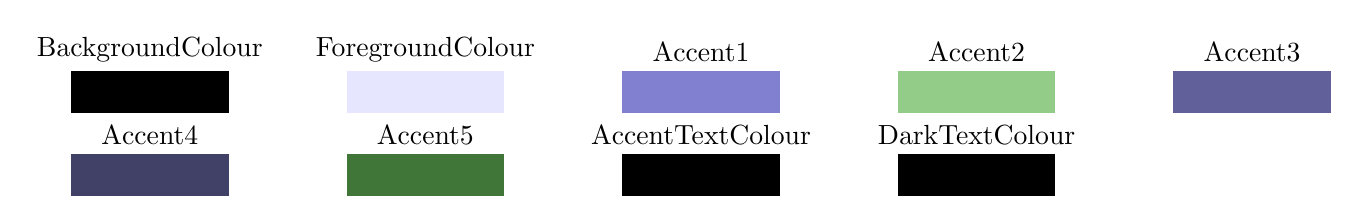
\begin{tikzpicture}
\definecolor{col}{HTML}{000000}
\fill[col] (0.0, -0.5em + 0em) rectangle (2.0, 1em + 0em) (1.0, 1em + 0em) node[above, text = black] {BackgroundColour};
\definecolor{col}{HTML}{E6E6FF}
\fill[col] (3.5, -0.5em + 0em) rectangle (5.5, 1em + 0em) (4.5, 1em + 0em) node[above, text = black] {ForegroundColour};
\definecolor{col}{HTML}{817FCF}
\fill[col] (7.0, -0.5em + 0em) rectangle (9.0, 1em + 0em) (8.0, 1em + 0em) node[above, text = black] {Accent1};
\definecolor{col}{HTML}{92CC88}
\fill[col] (10.5, -0.5em + 0em) rectangle (12.5, 1em + 0em) (11.5, 1em + 0em) node[above, text = black] {Accent2};
\definecolor{col}{HTML}{61609B}
\fill[col] (14.0, -0.5em + 0em) rectangle (16.0, 1em + 0em) (15.0, 1em + 0em) node[above, text = black] {Accent3};
\definecolor{col}{HTML}{414067}
\fill[col] (0.0, -0.5em + -3em) rectangle (2.0, 1em + -3em) (1.0, 1em + -3em) node[above, text = black] {Accent4};
\definecolor{col}{HTML}{417639}
\fill[col] (3.5, -0.5em + -3em) rectangle (5.5, 1em + -3em) (4.5, 1em + -3em) node[above, text = black] {Accent5};
\definecolor{col}{HTML}{000000}
\fill[col!50!black] (7.0, -0.5em + -3em) rectangle (9.0, 1em + -3em) (8.0, 1em + -3em) node[above, text = black] {AccentTextColour};
\definecolor{col}{HTML}{000000}
\fill[col!50!black] (10.5, -0.5em + -3em) rectangle (12.5, 1em + -3em) (11.5, 1em + -3em) node[above, text = black] {DarkTextColour};
\end{tikzpicture}

\subsection*{Bold}
\subsubsection*{Light}
\noindent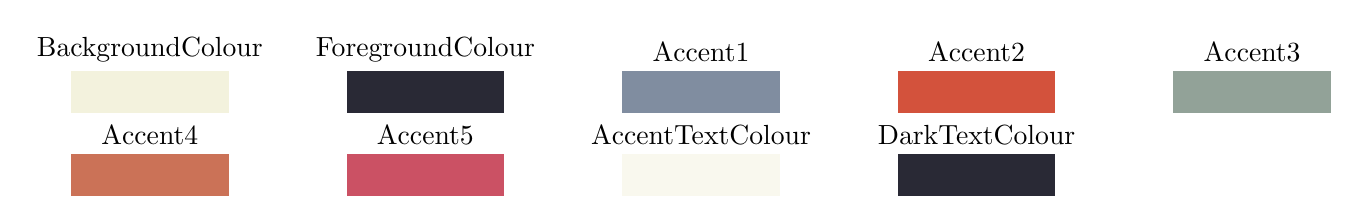
\begin{tikzpicture}
\definecolor{col}{HTML}{F3F2DD}
\fill[col] (0.0, -0.5em + 0em) rectangle (2.0, 1em + 0em) (1.0, 1em + 0em) node[above, text = black] {BackgroundColour};
\definecolor{col}{HTML}{292935}
\fill[col] (3.5, -0.5em + 0em) rectangle (5.5, 1em + 0em) (4.5, 1em + 0em) node[above, text = black] {ForegroundColour};
\definecolor{col}{HTML}{808DA0}
\fill[col] (7.0, -0.5em + 0em) rectangle (9.0, 1em + 0em) (8.0, 1em + 0em) node[above, text = black] {Accent1};
\definecolor{col}{HTML}{D3523C}
\fill[col] (10.5, -0.5em + 0em) rectangle (12.5, 1em + 0em) (11.5, 1em + 0em) node[above, text = black] {Accent2};
\definecolor{col}{HTML}{92A298}
\fill[col] (14.0, -0.5em + 0em) rectangle (16.0, 1em + 0em) (15.0, 1em + 0em) node[above, text = black] {Accent3};
\definecolor{col}{HTML}{CB7257}
\fill[col] (0.0, -0.5em + -3em) rectangle (2.0, 1em + -3em) (1.0, 1em + -3em) node[above, text = black] {Accent4};
\definecolor{col}{HTML}{CB5164}
\fill[col] (3.5, -0.5em + -3em) rectangle (5.5, 1em + -3em) (4.5, 1em + -3em) node[above, text = black] {Accent5};
\definecolor{col}{HTML}{F3F2DD}
\fill[col!50!white] (7.0, -0.5em + -3em) rectangle (9.0, 1em + -3em) (8.0, 1em + -3em) node[above, text = black] {AccentTextColour};
\definecolor{col}{HTML}{292935}
\fill[col] (10.5, -0.5em + -3em) rectangle (12.5, 1em + -3em) (11.5, 1em + -3em) node[above, text = black] {DarkTextColour};
\end{tikzpicture}

\subsubsection*{Dark}
\noindent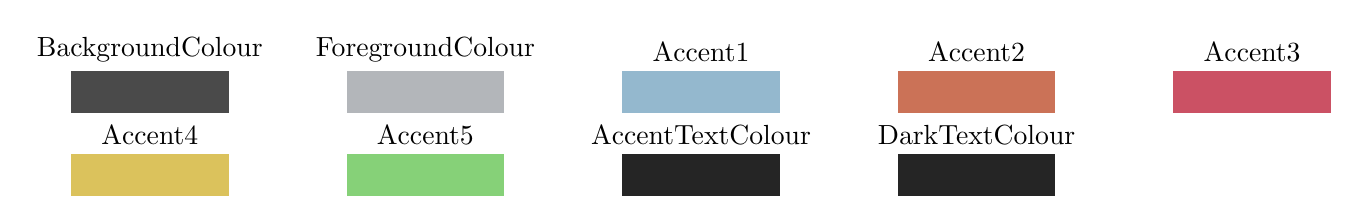
\begin{tikzpicture}
\definecolor{col}{HTML}{4A4A4A}
\fill[col] (0.0, -0.5em + 0em) rectangle (2.0, 1em + 0em) (1.0, 1em + 0em) node[above, text = black] {BackgroundColour};
\definecolor{col}{HTML}{B3B6BA}
\fill[col] (3.5, -0.5em + 0em) rectangle (5.5, 1em + 0em) (4.5, 1em + 0em) node[above, text = black] {ForegroundColour};
\definecolor{col}{HTML}{94B8CE}
\fill[col] (7.0, -0.5em + 0em) rectangle (9.0, 1em + 0em) (8.0, 1em + 0em) node[above, text = black] {Accent1};
\definecolor{col}{HTML}{CB7257}
\fill[col] (10.5, -0.5em + 0em) rectangle (12.5, 1em + 0em) (11.5, 1em + 0em) node[above, text = black] {Accent2};
\definecolor{col}{HTML}{CB5164}
\fill[col] (14.0, -0.5em + 0em) rectangle (16.0, 1em + 0em) (15.0, 1em + 0em) node[above, text = black] {Accent3};
\definecolor{col}{HTML}{DBC25C}
\fill[col] (0.0, -0.5em + -3em) rectangle (2.0, 1em + -3em) (1.0, 1em + -3em) node[above, text = black] {Accent4};
\definecolor{col}{HTML}{86D178}
\fill[col] (3.5, -0.5em + -3em) rectangle (5.5, 1em + -3em) (4.5, 1em + -3em) node[above, text = black] {Accent5};
\definecolor{col}{HTML}{4A4A4A}
\fill[col!50!black] (7.0, -0.5em + -3em) rectangle (9.0, 1em + -3em) (8.0, 1em + -3em) node[above, text = black] {AccentTextColour};
\definecolor{col}{HTML}{4A4A4A}
\fill[col!50!black] (10.5, -0.5em + -3em) rectangle (12.5, 1em + -3em) (11.5, 1em + -3em) node[above, text = black] {DarkTextColour};
\end{tikzpicture}

\subsection*{Sage}
\subsubsection*{Light}
\noindent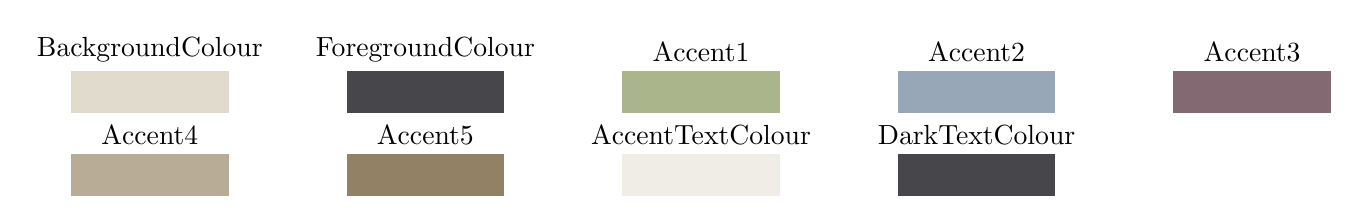
\begin{tikzpicture}
\definecolor{col}{HTML}{E1DBCE}
\fill[col] (0.0, -0.5em + 0em) rectangle (2.0, 1em + 0em) (1.0, 1em + 0em) node[above, text = black] {BackgroundColour};
\definecolor{col}{HTML}{47474B}
\fill[col] (3.5, -0.5em + 0em) rectangle (5.5, 1em + 0em) (4.5, 1em + 0em) node[above, text = black] {ForegroundColour};
\definecolor{col}{HTML}{AAB58B}
\fill[col] (7.0, -0.5em + 0em) rectangle (9.0, 1em + 0em) (8.0, 1em + 0em) node[above, text = black] {Accent1};
\definecolor{col}{HTML}{97A7B7}
\fill[col] (10.5, -0.5em + 0em) rectangle (12.5, 1em + 0em) (11.5, 1em + 0em) node[above, text = black] {Accent2};
\definecolor{col}{HTML}{836972}
\fill[col] (14.0, -0.5em + 0em) rectangle (16.0, 1em + 0em) (15.0, 1em + 0em) node[above, text = black] {Accent3};
\definecolor{col}{HTML}{B8AC97}
\fill[col] (0.0, -0.5em + -3em) rectangle (2.0, 1em + -3em) (1.0, 1em + -3em) node[above, text = black] {Accent4};
\definecolor{col}{HTML}{938165}
\fill[col] (3.5, -0.5em + -3em) rectangle (5.5, 1em + -3em) (4.5, 1em + -3em) node[above, text = black] {Accent5};
\definecolor{col}{HTML}{E1DBCE}
\fill[col!50!white] (7.0, -0.5em + -3em) rectangle (9.0, 1em + -3em) (8.0, 1em + -3em) node[above, text = black] {AccentTextColour};
\definecolor{col}{HTML}{47474B}
\fill[col] (10.5, -0.5em + -3em) rectangle (12.5, 1em + -3em) (11.5, 1em + -3em) node[above, text = black] {DarkTextColour};
\end{tikzpicture}

\subsubsection*{Dark}
\noindent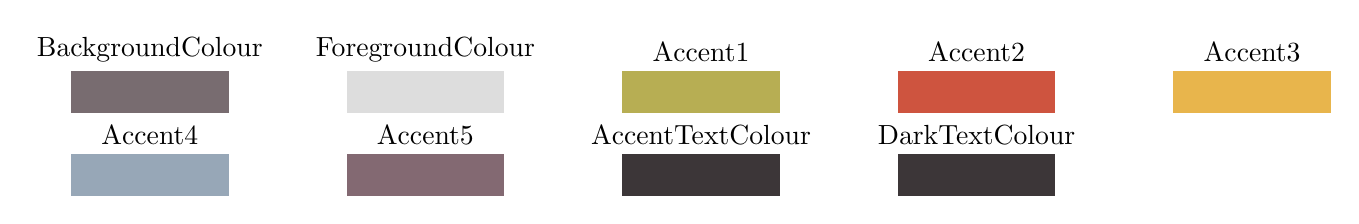
\begin{tikzpicture}
\definecolor{col}{HTML}{786C70}
\fill[col] (0.0, -0.5em + 0em) rectangle (2.0, 1em + 0em) (1.0, 1em + 0em) node[above, text = black] {BackgroundColour};
\definecolor{col}{HTML}{DDDDDD}
\fill[col] (3.5, -0.5em + 0em) rectangle (5.5, 1em + 0em) (4.5, 1em + 0em) node[above, text = black] {ForegroundColour};
\definecolor{col}{HTML}{B7AE53}
\fill[col] (7.0, -0.5em + 0em) rectangle (9.0, 1em + 0em) (8.0, 1em + 0em) node[above, text = black] {Accent1};
\definecolor{col}{HTML}{CE543F}
\fill[col] (10.5, -0.5em + 0em) rectangle (12.5, 1em + 0em) (11.5, 1em + 0em) node[above, text = black] {Accent2};
\definecolor{col}{HTML}{E8B54C}
\fill[col] (14.0, -0.5em + 0em) rectangle (16.0, 1em + 0em) (15.0, 1em + 0em) node[above, text = black] {Accent3};
\definecolor{col}{HTML}{97A7B7}
\fill[col] (0.0, -0.5em + -3em) rectangle (2.0, 1em + -3em) (1.0, 1em + -3em) node[above, text = black] {Accent4};
\definecolor{col}{HTML}{836972}
\fill[col] (3.5, -0.5em + -3em) rectangle (5.5, 1em + -3em) (4.5, 1em + -3em) node[above, text = black] {Accent5};
\definecolor{col}{HTML}{786C70}
\fill[col!50!black] (7.0, -0.5em + -3em) rectangle (9.0, 1em + -3em) (8.0, 1em + -3em) node[above, text = black] {AccentTextColour};
\definecolor{col}{HTML}{786C70}
\fill[col!50!black] (10.5, -0.5em + -3em) rectangle (12.5, 1em + -3em) (11.5, 1em + -3em) node[above, text = black] {DarkTextColour};
\end{tikzpicture}

\subsection*{Succulent}
\subsubsection*{Dark}
\noindent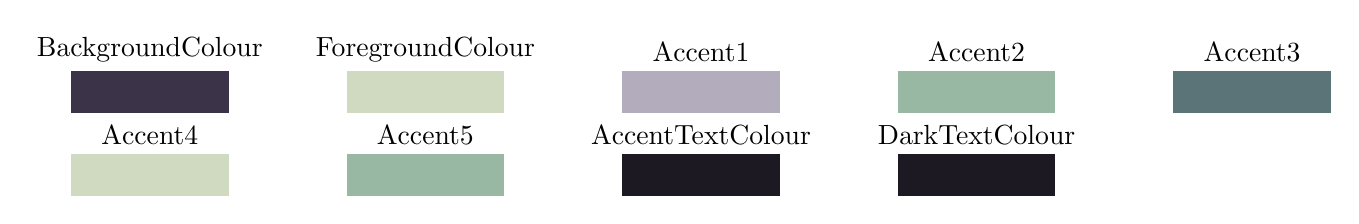
\begin{tikzpicture}
\definecolor{col}{HTML}{3B3347}
\fill[col] (0.0, -0.5em + 0em) rectangle (2.0, 1em + 0em) (1.0, 1em + 0em) node[above, text = black] {BackgroundColour};
\definecolor{col}{HTML}{D0DAC0}
\fill[col] (3.5, -0.5em + 0em) rectangle (5.5, 1em + 0em) (4.5, 1em + 0em) node[above, text = black] {ForegroundColour};
\definecolor{col}{HTML}{B3ACBD}
\fill[col] (7.0, -0.5em + 0em) rectangle (9.0, 1em + 0em) (8.0, 1em + 0em) node[above, text = black] {Accent1};
\definecolor{col}{HTML}{99B8A4}
\fill[col] (10.5, -0.5em + 0em) rectangle (12.5, 1em + 0em) (11.5, 1em + 0em) node[above, text = black] {Accent2};
\definecolor{col}{HTML}{5A7477}
\fill[col] (14.0, -0.5em + 0em) rectangle (16.0, 1em + 0em) (15.0, 1em + 0em) node[above, text = black] {Accent3};
\definecolor{col}{HTML}{D0DAC0}
\fill[col] (0.0, -0.5em + -3em) rectangle (2.0, 1em + -3em) (1.0, 1em + -3em) node[above, text = black] {Accent4};
\definecolor{col}{HTML}{99B8A4}
\fill[col] (3.5, -0.5em + -3em) rectangle (5.5, 1em + -3em) (4.5, 1em + -3em) node[above, text = black] {Accent5};
\definecolor{col}{HTML}{3B3347}
\fill[col!50!black] (7.0, -0.5em + -3em) rectangle (9.0, 1em + -3em) (8.0, 1em + -3em) node[above, text = black] {AccentTextColour};
\definecolor{col}{HTML}{3B3347}
\fill[col!50!black] (10.5, -0.5em + -3em) rectangle (12.5, 1em + -3em) (11.5, 1em + -3em) node[above, text = black] {DarkTextColour};
\end{tikzpicture}

\subsection*{Muted}
\subsubsection*{Light}
\noindent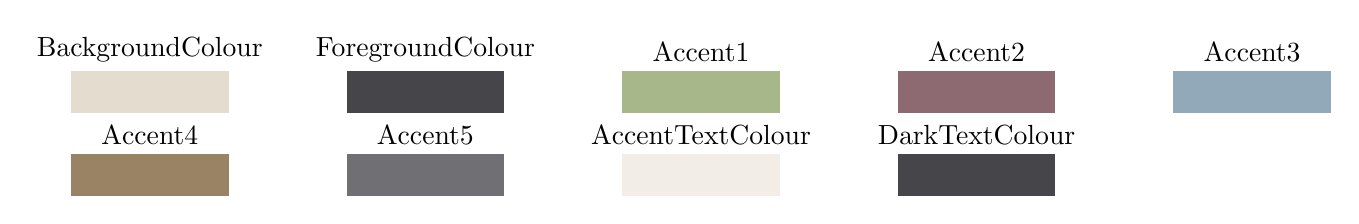
\begin{tikzpicture}
\definecolor{col}{HTML}{E4DCCF}
\fill[col] (0.0, -0.5em + 0em) rectangle (2.0, 1em + 0em) (1.0, 1em + 0em) node[above, text = black] {BackgroundColour};
\definecolor{col}{HTML}{46454A}
\fill[col] (3.5, -0.5em + 0em) rectangle (5.5, 1em + 0em) (4.5, 1em + 0em) node[above, text = black] {ForegroundColour};
\definecolor{col}{HTML}{A7B78A}
\fill[col] (7.0, -0.5em + 0em) rectangle (9.0, 1em + 0em) (8.0, 1em + 0em) node[above, text = black] {Accent1};
\definecolor{col}{HTML}{8D6972}
\fill[col] (10.5, -0.5em + 0em) rectangle (12.5, 1em + 0em) (11.5, 1em + 0em) node[above, text = black] {Accent2};
\definecolor{col}{HTML}{92A9B9}
\fill[col] (14.0, -0.5em + 0em) rectangle (16.0, 1em + 0em) (15.0, 1em + 0em) node[above, text = black] {Accent3};
\definecolor{col}{HTML}{9A8264}
\fill[col] (0.0, -0.5em + -3em) rectangle (2.0, 1em + -3em) (1.0, 1em + -3em) node[above, text = black] {Accent4};
\definecolor{col}{HTML}{706F73}
\fill[col] (3.5, -0.5em + -3em) rectangle (5.5, 1em + -3em) (4.5, 1em + -3em) node[above, text = black] {Accent5};
\definecolor{col}{HTML}{E4DCCF}
\fill[col!50!white] (7.0, -0.5em + -3em) rectangle (9.0, 1em + -3em) (8.0, 1em + -3em) node[above, text = black] {AccentTextColour};
\definecolor{col}{HTML}{46454A}
\fill[col] (10.5, -0.5em + -3em) rectangle (12.5, 1em + -3em) (11.5, 1em + -3em) node[above, text = black] {DarkTextColour};
\end{tikzpicture}

\subsection*{Office 2011}
\subsubsection*{Light}
\noindent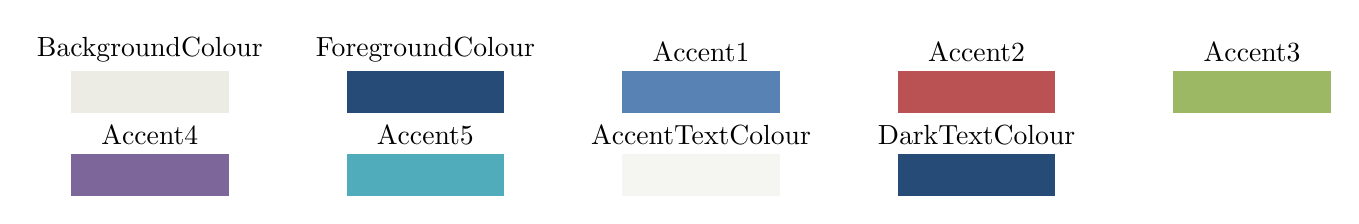
\begin{tikzpicture}
\definecolor{col}{HTML}{ECECE4}
\fill[col] (0.0, -0.5em + 0em) rectangle (2.0, 1em + 0em) (1.0, 1em + 0em) node[above, text = black] {BackgroundColour};
\definecolor{col}{HTML}{264B77}
\fill[col] (3.5, -0.5em + 0em) rectangle (5.5, 1em + 0em) (4.5, 1em + 0em) node[above, text = black] {ForegroundColour};
\definecolor{col}{HTML}{5882B4}
\fill[col] (7.0, -0.5em + 0em) rectangle (9.0, 1em + 0em) (8.0, 1em + 0em) node[above, text = black] {Accent1};
\definecolor{col}{HTML}{BA5253}
\fill[col] (10.5, -0.5em + 0em) rectangle (12.5, 1em + 0em) (11.5, 1em + 0em) node[above, text = black] {Accent2};
\definecolor{col}{HTML}{9CB864}
\fill[col] (14.0, -0.5em + 0em) rectangle (16.0, 1em + 0em) (15.0, 1em + 0em) node[above, text = black] {Accent3};
\definecolor{col}{HTML}{7D669A}
\fill[col] (0.0, -0.5em + -3em) rectangle (2.0, 1em + -3em) (1.0, 1em + -3em) node[above, text = black] {Accent4};
\definecolor{col}{HTML}{50ACBB}
\fill[col] (3.5, -0.5em + -3em) rectangle (5.5, 1em + -3em) (4.5, 1em + -3em) node[above, text = black] {Accent5};
\definecolor{col}{HTML}{ECECE4}
\fill[col!50!white] (7.0, -0.5em + -3em) rectangle (9.0, 1em + -3em) (8.0, 1em + -3em) node[above, text = black] {AccentTextColour};
\definecolor{col}{HTML}{264B77}
\fill[col] (10.5, -0.5em + -3em) rectangle (12.5, 1em + -3em) (11.5, 1em + -3em) node[above, text = black] {DarkTextColour};
\end{tikzpicture}

\subsection*{Grayscale}
\subsubsection*{Light}
\noindent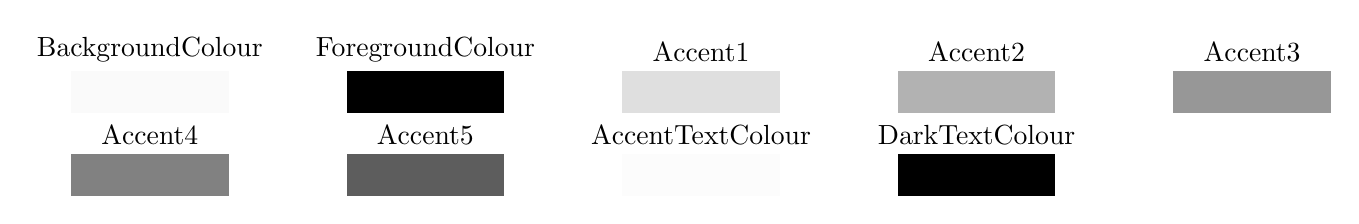
\begin{tikzpicture}
\definecolor{col}{HTML}{FAFAFA}
\fill[col] (0.0, -0.5em + 0em) rectangle (2.0, 1em + 0em) (1.0, 1em + 0em) node[above, text = black] {BackgroundColour};
\definecolor{col}{HTML}{000000}
\fill[col] (3.5, -0.5em + 0em) rectangle (5.5, 1em + 0em) (4.5, 1em + 0em) node[above, text = black] {ForegroundColour};
\definecolor{col}{HTML}{DFDFDF}
\fill[col] (7.0, -0.5em + 0em) rectangle (9.0, 1em + 0em) (8.0, 1em + 0em) node[above, text = black] {Accent1};
\definecolor{col}{HTML}{B2B2B2}
\fill[col] (10.5, -0.5em + 0em) rectangle (12.5, 1em + 0em) (11.5, 1em + 0em) node[above, text = black] {Accent2};
\definecolor{col}{HTML}{979797}
\fill[col] (14.0, -0.5em + 0em) rectangle (16.0, 1em + 0em) (15.0, 1em + 0em) node[above, text = black] {Accent3};
\definecolor{col}{HTML}{818181}
\fill[col] (0.0, -0.5em + -3em) rectangle (2.0, 1em + -3em) (1.0, 1em + -3em) node[above, text = black] {Accent4};
\definecolor{col}{HTML}{5D5D5D}
\fill[col] (3.5, -0.5em + -3em) rectangle (5.5, 1em + -3em) (4.5, 1em + -3em) node[above, text = black] {Accent5};
\definecolor{col}{HTML}{FAFAFA}
\fill[col!50!white] (7.0, -0.5em + -3em) rectangle (9.0, 1em + -3em) (8.0, 1em + -3em) node[above, text = black] {AccentTextColour};
\definecolor{col}{HTML}{000000}
\fill[col] (10.5, -0.5em + -3em) rectangle (12.5, 1em + -3em) (11.5, 1em + -3em) node[above, text = black] {DarkTextColour};
\end{tikzpicture}

\subsection*{Adjacency}
\subsubsection*{Light}
\noindent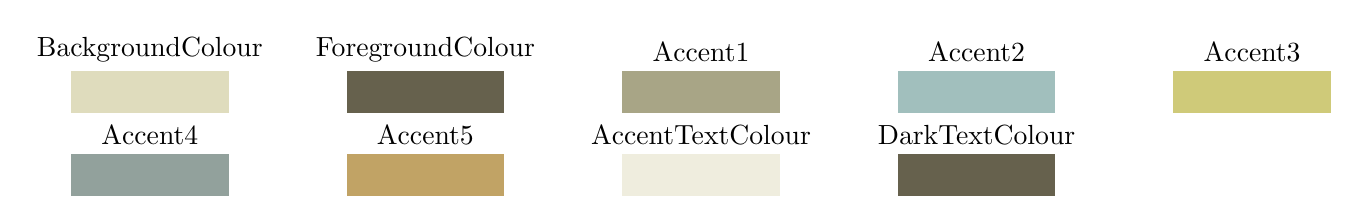
\begin{tikzpicture}
\definecolor{col}{HTML}{DFDCBD}
\fill[col] (0.0, -0.5em + 0em) rectangle (2.0, 1em + 0em) (1.0, 1em + 0em) node[above, text = black] {BackgroundColour};
\definecolor{col}{HTML}{66614D}
\fill[col] (3.5, -0.5em + 0em) rectangle (5.5, 1em + 0em) (4.5, 1em + 0em) node[above, text = black] {ForegroundColour};
\definecolor{col}{HTML}{A8A586}
\fill[col] (7.0, -0.5em + 0em) rectangle (9.0, 1em + 0em) (8.0, 1em + 0em) node[above, text = black] {Accent1};
\definecolor{col}{HTML}{A1BFBD}
\fill[col] (10.5, -0.5em + 0em) rectangle (12.5, 1em + 0em) (11.5, 1em + 0em) node[above, text = black] {Accent2};
\definecolor{col}{HTML}{CFCA79}
\fill[col] (14.0, -0.5em + 0em) rectangle (16.0, 1em + 0em) (15.0, 1em + 0em) node[above, text = black] {Accent3};
\definecolor{col}{HTML}{92A19C}
\fill[col] (0.0, -0.5em + -3em) rectangle (2.0, 1em + -3em) (1.0, 1em + -3em) node[above, text = black] {Accent4};
\definecolor{col}{HTML}{C1A365}
\fill[col] (3.5, -0.5em + -3em) rectangle (5.5, 1em + -3em) (4.5, 1em + -3em) node[above, text = black] {Accent5};
\definecolor{col}{HTML}{DFDCBD}
\fill[col!50!white] (7.0, -0.5em + -3em) rectangle (9.0, 1em + -3em) (8.0, 1em + -3em) node[above, text = black] {AccentTextColour};
\definecolor{col}{HTML}{66614D}
\fill[col] (10.5, -0.5em + -3em) rectangle (12.5, 1em + -3em) (11.5, 1em + -3em) node[above, text = black] {DarkTextColour};
\end{tikzpicture}

\subsection*{Advantage}
\subsubsection*{Light}
\noindent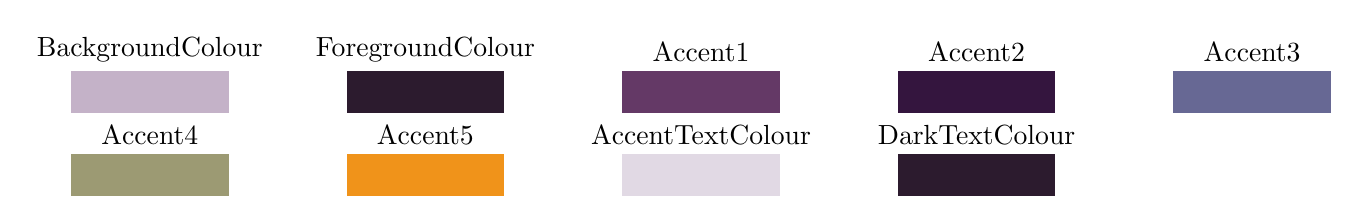
\begin{tikzpicture}
\definecolor{col}{HTML}{C4B2C8}
\fill[col] (0.0, -0.5em + 0em) rectangle (2.0, 1em + 0em) (1.0, 1em + 0em) node[above, text = black] {BackgroundColour};
\definecolor{col}{HTML}{2C1B2E}
\fill[col] (3.5, -0.5em + 0em) rectangle (5.5, 1em + 0em) (4.5, 1em + 0em) node[above, text = black] {ForegroundColour};
\definecolor{col}{HTML}{643966}
\fill[col] (7.0, -0.5em + 0em) rectangle (9.0, 1em + 0em) (8.0, 1em + 0em) node[above, text = black] {Accent1};
\definecolor{col}{HTML}{34153E}
\fill[col] (10.5, -0.5em + 0em) rectangle (12.5, 1em + 0em) (11.5, 1em + 0em) node[above, text = black] {Accent2};
\definecolor{col}{HTML}{676894}
\fill[col] (14.0, -0.5em + 0em) rectangle (16.0, 1em + 0em) (15.0, 1em + 0em) node[above, text = black] {Accent3};
\definecolor{col}{HTML}{9C9A73}
\fill[col] (0.0, -0.5em + -3em) rectangle (2.0, 1em + -3em) (1.0, 1em + -3em) node[above, text = black] {Accent4};
\definecolor{col}{HTML}{F0931A}
\fill[col] (3.5, -0.5em + -3em) rectangle (5.5, 1em + -3em) (4.5, 1em + -3em) node[above, text = black] {Accent5};
\definecolor{col}{HTML}{C4B2C8}
\fill[col!50!white] (7.0, -0.5em + -3em) rectangle (9.0, 1em + -3em) (8.0, 1em + -3em) node[above, text = black] {AccentTextColour};
\definecolor{col}{HTML}{2C1B2E}
\fill[col] (10.5, -0.5em + -3em) rectangle (12.5, 1em + -3em) (11.5, 1em + -3em) node[above, text = black] {DarkTextColour};
\end{tikzpicture}

\subsection*{Angeles}
\subsubsection*{Light}
\noindent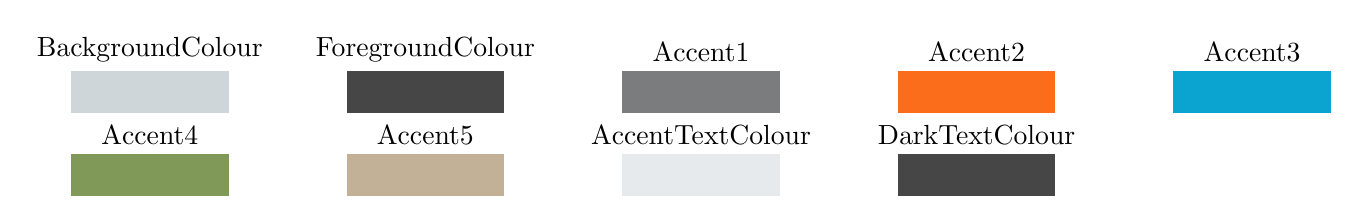
\begin{tikzpicture}
\definecolor{col}{HTML}{CED6D9}
\fill[col] (0.0, -0.5em + 0em) rectangle (2.0, 1em + 0em) (1.0, 1em + 0em) node[above, text = black] {BackgroundColour};
\definecolor{col}{HTML}{464646}
\fill[col] (3.5, -0.5em + 0em) rectangle (5.5, 1em + 0em) (4.5, 1em + 0em) node[above, text = black] {ForegroundColour};
\definecolor{col}{HTML}{7B7C7E}
\fill[col] (7.0, -0.5em + 0em) rectangle (9.0, 1em + 0em) (8.0, 1em + 0em) node[above, text = black] {Accent1};
\definecolor{col}{HTML}{FB6D1B}
\fill[col] (10.5, -0.5em + 0em) rectangle (12.5, 1em + 0em) (11.5, 1em + 0em) node[above, text = black] {Accent2};
\definecolor{col}{HTML}{0BA4D0}
\fill[col] (14.0, -0.5em + 0em) rectangle (16.0, 1em + 0em) (15.0, 1em + 0em) node[above, text = black] {Accent3};
\definecolor{col}{HTML}{809958}
\fill[col] (0.0, -0.5em + -3em) rectangle (2.0, 1em + -3em) (1.0, 1em + -3em) node[above, text = black] {Accent4};
\definecolor{col}{HTML}{C2B197}
\fill[col] (3.5, -0.5em + -3em) rectangle (5.5, 1em + -3em) (4.5, 1em + -3em) node[above, text = black] {Accent5};
\definecolor{col}{HTML}{CED6D9}
\fill[col!50!white] (7.0, -0.5em + -3em) rectangle (9.0, 1em + -3em) (8.0, 1em + -3em) node[above, text = black] {AccentTextColour};
\definecolor{col}{HTML}{464646}
\fill[col] (10.5, -0.5em + -3em) rectangle (12.5, 1em + -3em) (11.5, 1em + -3em) node[above, text = black] {DarkTextColour};
\end{tikzpicture}

\subsection*{Apothecary}
\subsubsection*{Light}
\noindent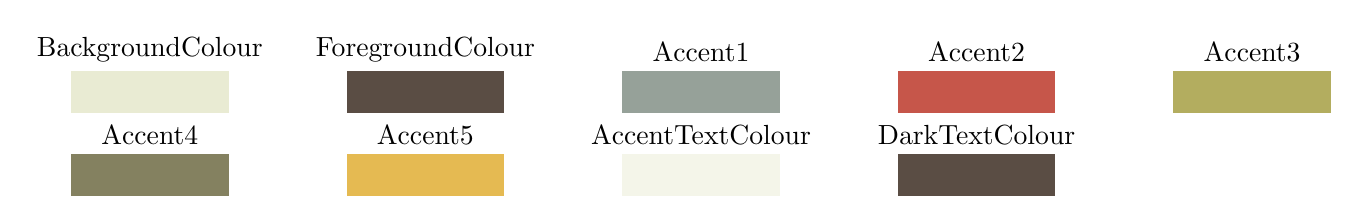
\begin{tikzpicture}
\definecolor{col}{HTML}{E9EBD3}
\fill[col] (0.0, -0.5em + 0em) rectangle (2.0, 1em + 0em) (1.0, 1em + 0em) node[above, text = black] {BackgroundColour};
\definecolor{col}{HTML}{5A4D44}
\fill[col] (3.5, -0.5em + 0em) rectangle (5.5, 1em + 0em) (4.5, 1em + 0em) node[above, text = black] {ForegroundColour};
\definecolor{col}{HTML}{96A199}
\fill[col] (7.0, -0.5em + 0em) rectangle (9.0, 1em + 0em) (8.0, 1em + 0em) node[above, text = black] {Accent1};
\definecolor{col}{HTML}{C6564A}
\fill[col] (10.5, -0.5em + 0em) rectangle (12.5, 1em + 0em) (11.5, 1em + 0em) node[above, text = black] {Accent2};
\definecolor{col}{HTML}{B3AD5F}
\fill[col] (14.0, -0.5em + 0em) rectangle (16.0, 1em + 0em) (15.0, 1em + 0em) node[above, text = black] {Accent3};
\definecolor{col}{HTML}{848160}
\fill[col] (0.0, -0.5em + -3em) rectangle (2.0, 1em + -3em) (1.0, 1em + -3em) node[above, text = black] {Accent4};
\definecolor{col}{HTML}{E5BA52}
\fill[col] (3.5, -0.5em + -3em) rectangle (5.5, 1em + -3em) (4.5, 1em + -3em) node[above, text = black] {Accent5};
\definecolor{col}{HTML}{E9EBD3}
\fill[col!50!white] (7.0, -0.5em + -3em) rectangle (9.0, 1em + -3em) (8.0, 1em + -3em) node[above, text = black] {AccentTextColour};
\definecolor{col}{HTML}{5A4D44}
\fill[col] (10.5, -0.5em + -3em) rectangle (12.5, 1em + -3em) (11.5, 1em + -3em) node[above, text = black] {DarkTextColour};
\end{tikzpicture}

\subsection*{Austin}
\subsubsection*{Light}
\noindent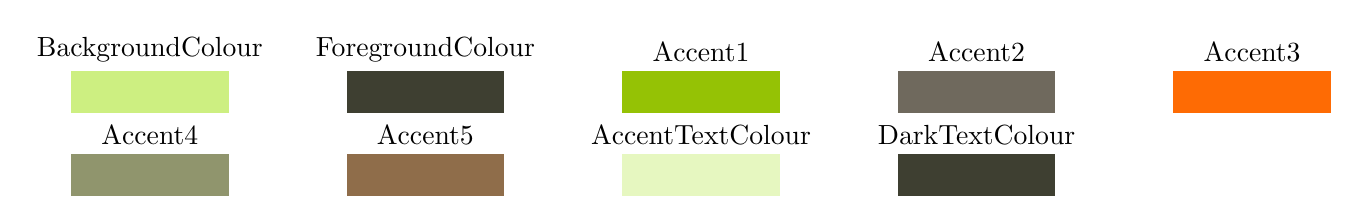
\begin{tikzpicture}
\definecolor{col}{HTML}{CDEF81}
\fill[col] (0.0, -0.5em + 0em) rectangle (2.0, 1em + 0em) (1.0, 1em + 0em) node[above, text = black] {BackgroundColour};
\definecolor{col}{HTML}{3E3F31}
\fill[col] (3.5, -0.5em + 0em) rectangle (5.5, 1em + 0em) (4.5, 1em + 0em) node[above, text = black] {ForegroundColour};
\definecolor{col}{HTML}{95C205}
\fill[col] (7.0, -0.5em + 0em) rectangle (9.0, 1em + 0em) (8.0, 1em + 0em) node[above, text = black] {Accent1};
\definecolor{col}{HTML}{6F695D}
\fill[col] (10.5, -0.5em + 0em) rectangle (12.5, 1em + 0em) (11.5, 1em + 0em) node[above, text = black] {Accent2};
\definecolor{col}{HTML}{FE6B04}
\fill[col] (14.0, -0.5em + 0em) rectangle (16.0, 1em + 0em) (15.0, 1em + 0em) node[above, text = black] {Accent3};
\definecolor{col}{HTML}{90956D}
\fill[col] (0.0, -0.5em + -3em) rectangle (2.0, 1em + -3em) (1.0, 1em + -3em) node[above, text = black] {Accent4};
\definecolor{col}{HTML}{8F6D4A}
\fill[col] (3.5, -0.5em + -3em) rectangle (5.5, 1em + -3em) (4.5, 1em + -3em) node[above, text = black] {Accent5};
\definecolor{col}{HTML}{CDEF81}
\fill[col!50!white] (7.0, -0.5em + -3em) rectangle (9.0, 1em + -3em) (8.0, 1em + -3em) node[above, text = black] {AccentTextColour};
\definecolor{col}{HTML}{3E3F31}
\fill[col] (10.5, -0.5em + -3em) rectangle (12.5, 1em + -3em) (11.5, 1em + -3em) node[above, text = black] {DarkTextColour};
\end{tikzpicture}

\subsection*{Black Tie}
\subsubsection*{Light}
\noindent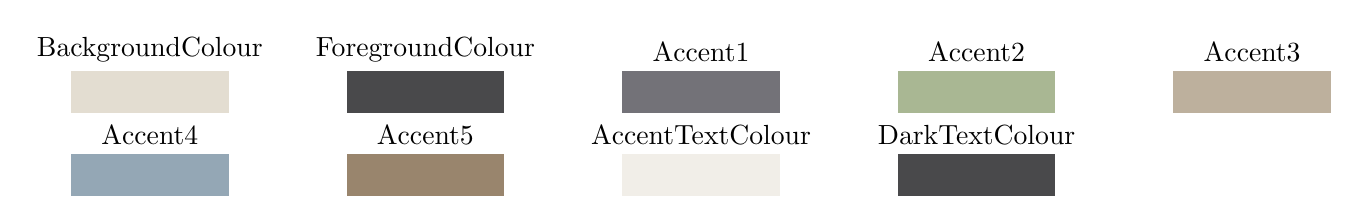
\begin{tikzpicture}
\definecolor{col}{HTML}{E3DDD1}
\fill[col] (0.0, -0.5em + 0em) rectangle (2.0, 1em + 0em) (1.0, 1em + 0em) node[above, text = black] {BackgroundColour};
\definecolor{col}{HTML}{49494B}
\fill[col] (3.5, -0.5em + 0em) rectangle (5.5, 1em + 0em) (4.5, 1em + 0em) node[above, text = black] {ForegroundColour};
\definecolor{col}{HTML}{737278}
\fill[col] (7.0, -0.5em + 0em) rectangle (9.0, 1em + 0em) (8.0, 1em + 0em) node[above, text = black] {Accent1};
\definecolor{col}{HTML}{A9B793}
\fill[col] (10.5, -0.5em + 0em) rectangle (12.5, 1em + 0em) (11.5, 1em + 0em) node[above, text = black] {Accent2};
\definecolor{col}{HTML}{BDB09D}
\fill[col] (14.0, -0.5em + 0em) rectangle (16.0, 1em + 0em) (15.0, 1em + 0em) node[above, text = black] {Accent3};
\definecolor{col}{HTML}{94A7B5}
\fill[col] (0.0, -0.5em + -3em) rectangle (2.0, 1em + -3em) (1.0, 1em + -3em) node[above, text = black] {Accent4};
\definecolor{col}{HTML}{99856D}
\fill[col] (3.5, -0.5em + -3em) rectangle (5.5, 1em + -3em) (4.5, 1em + -3em) node[above, text = black] {Accent5};
\definecolor{col}{HTML}{E3DDD1}
\fill[col!50!white] (7.0, -0.5em + -3em) rectangle (9.0, 1em + -3em) (8.0, 1em + -3em) node[above, text = black] {AccentTextColour};
\definecolor{col}{HTML}{49494B}
\fill[col] (10.5, -0.5em + -3em) rectangle (12.5, 1em + -3em) (11.5, 1em + -3em) node[above, text = black] {DarkTextColour};
\end{tikzpicture}

\subsection*{Breeze}
\subsubsection*{Light}
\noindent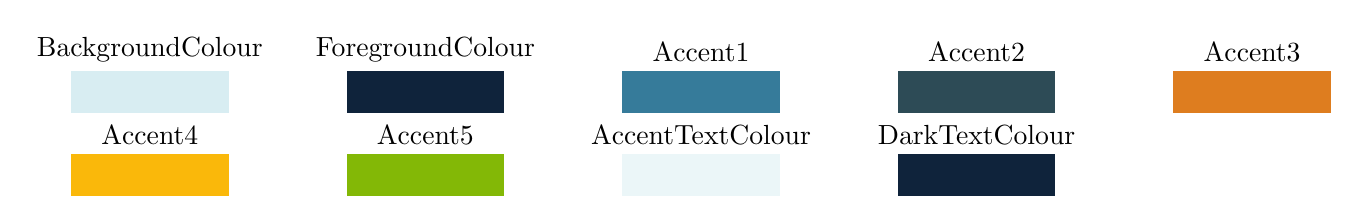
\begin{tikzpicture}
\definecolor{col}{HTML}{D8EDF2}
\fill[col] (0.0, -0.5em + 0em) rectangle (2.0, 1em + 0em) (1.0, 1em + 0em) node[above, text = black] {BackgroundColour};
\definecolor{col}{HTML}{0F233B}
\fill[col] (3.5, -0.5em + 0em) rectangle (5.5, 1em + 0em) (4.5, 1em + 0em) node[above, text = black] {ForegroundColour};
\definecolor{col}{HTML}{367B9A}
\fill[col] (7.0, -0.5em + 0em) rectangle (9.0, 1em + 0em) (8.0, 1em + 0em) node[above, text = black] {Accent1};
\definecolor{col}{HTML}{2D4B56}
\fill[col] (10.5, -0.5em + 0em) rectangle (12.5, 1em + 0em) (11.5, 1em + 0em) node[above, text = black] {Accent2};
\definecolor{col}{HTML}{DE7D1F}
\fill[col] (14.0, -0.5em + 0em) rectangle (16.0, 1em + 0em) (15.0, 1em + 0em) node[above, text = black] {Accent3};
\definecolor{col}{HTML}{FAB80A}
\fill[col] (0.0, -0.5em + -3em) rectangle (2.0, 1em + -3em) (1.0, 1em + -3em) node[above, text = black] {Accent4};
\definecolor{col}{HTML}{83B806}
\fill[col] (3.5, -0.5em + -3em) rectangle (5.5, 1em + -3em) (4.5, 1em + -3em) node[above, text = black] {Accent5};
\definecolor{col}{HTML}{D8EDF2}
\fill[col!50!white] (7.0, -0.5em + -3em) rectangle (9.0, 1em + -3em) (8.0, 1em + -3em) node[above, text = black] {AccentTextColour};
\definecolor{col}{HTML}{0F233B}
\fill[col] (10.5, -0.5em + -3em) rectangle (12.5, 1em + -3em) (11.5, 1em + -3em) node[above, text = black] {DarkTextColour};
\end{tikzpicture}

\subsection*{Capital}
\subsubsection*{Light}
\noindent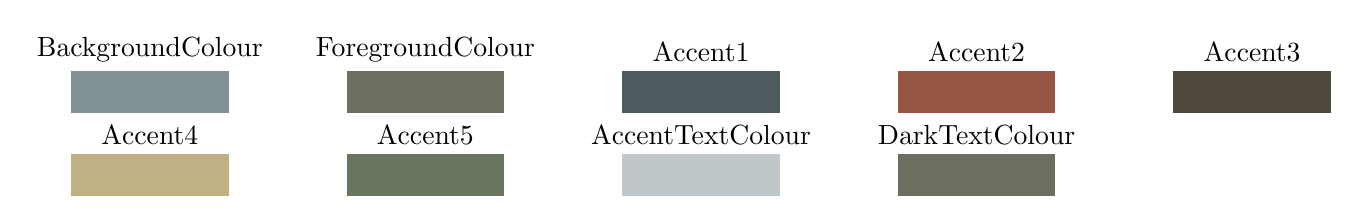
\begin{tikzpicture}
\definecolor{col}{HTML}{819095}
\fill[col] (0.0, -0.5em + 0em) rectangle (2.0, 1em + 0em) (1.0, 1em + 0em) node[above, text = black] {BackgroundColour};
\definecolor{col}{HTML}{6D6E60}
\fill[col] (3.5, -0.5em + 0em) rectangle (5.5, 1em + 0em) (4.5, 1em + 0em) node[above, text = black] {ForegroundColour};
\definecolor{col}{HTML}{4D5B5E}
\fill[col] (7.0, -0.5em + 0em) rectangle (9.0, 1em + 0em) (8.0, 1em + 0em) node[above, text = black] {Accent1};
\definecolor{col}{HTML}{945543}
\fill[col] (10.5, -0.5em + 0em) rectangle (12.5, 1em + 0em) (11.5, 1em + 0em) node[above, text = black] {Accent2};
\definecolor{col}{HTML}{4F493D}
\fill[col] (14.0, -0.5em + 0em) rectangle (16.0, 1em + 0em) (15.0, 1em + 0em) node[above, text = black] {Accent3};
\definecolor{col}{HTML}{C1B084}
\fill[col] (0.0, -0.5em + -3em) rectangle (2.0, 1em + -3em) (1.0, 1em + -3em) node[above, text = black] {Accent4};
\definecolor{col}{HTML}{69755F}
\fill[col] (3.5, -0.5em + -3em) rectangle (5.5, 1em + -3em) (4.5, 1em + -3em) node[above, text = black] {Accent5};
\definecolor{col}{HTML}{819095}
\fill[col!50!white] (7.0, -0.5em + -3em) rectangle (9.0, 1em + -3em) (8.0, 1em + -3em) node[above, text = black] {AccentTextColour};
\definecolor{col}{HTML}{6D6E60}
\fill[col] (10.5, -0.5em + -3em) rectangle (12.5, 1em + -3em) (11.5, 1em + -3em) node[above, text = black] {DarkTextColour};
\end{tikzpicture}

\subsection*{Civic}
\subsubsection*{Light}
\noindent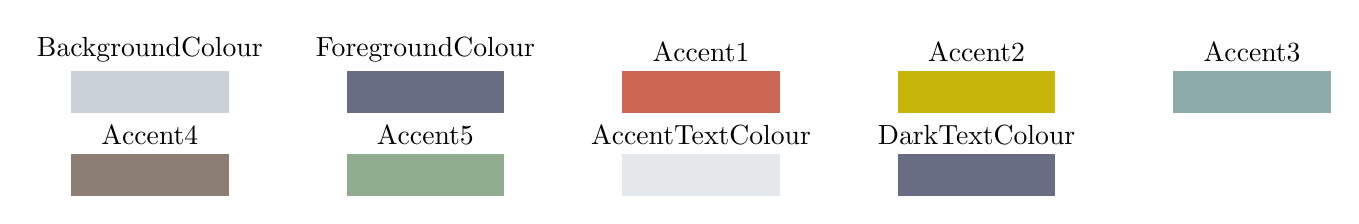
\begin{tikzpicture}
\definecolor{col}{HTML}{CAD1D7}
\fill[col] (0.0, -0.5em + 0em) rectangle (2.0, 1em + 0em) (1.0, 1em + 0em) node[above, text = black] {BackgroundColour};
\definecolor{col}{HTML}{686D83}
\fill[col] (3.5, -0.5em + 0em) rectangle (5.5, 1em + 0em) (4.5, 1em + 0em) node[above, text = black] {ForegroundColour};
\definecolor{col}{HTML}{CD6653}
\fill[col] (7.0, -0.5em + 0em) rectangle (9.0, 1em + 0em) (8.0, 1em + 0em) node[above, text = black] {Accent1};
\definecolor{col}{HTML}{C7B509}
\fill[col] (10.5, -0.5em + 0em) rectangle (12.5, 1em + 0em) (11.5, 1em + 0em) node[above, text = black] {Accent2};
\definecolor{col}{HTML}{8DABA9}
\fill[col] (14.0, -0.5em + 0em) rectangle (16.0, 1em + 0em) (15.0, 1em + 0em) node[above, text = black] {Accent3};
\definecolor{col}{HTML}{8C7E75}
\fill[col] (0.0, -0.5em + -3em) rectangle (2.0, 1em + -3em) (1.0, 1em + -3em) node[above, text = black] {Accent4};
\definecolor{col}{HTML}{90AD8F}
\fill[col] (3.5, -0.5em + -3em) rectangle (5.5, 1em + -3em) (4.5, 1em + -3em) node[above, text = black] {Accent5};
\definecolor{col}{HTML}{CAD1D7}
\fill[col!50!white] (7.0, -0.5em + -3em) rectangle (9.0, 1em + -3em) (8.0, 1em + -3em) node[above, text = black] {AccentTextColour};
\definecolor{col}{HTML}{686D83}
\fill[col] (10.5, -0.5em + -3em) rectangle (12.5, 1em + -3em) (11.5, 1em + -3em) node[above, text = black] {DarkTextColour};
\end{tikzpicture}

\subsection*{Clarity}
\subsubsection*{Light}
\noindent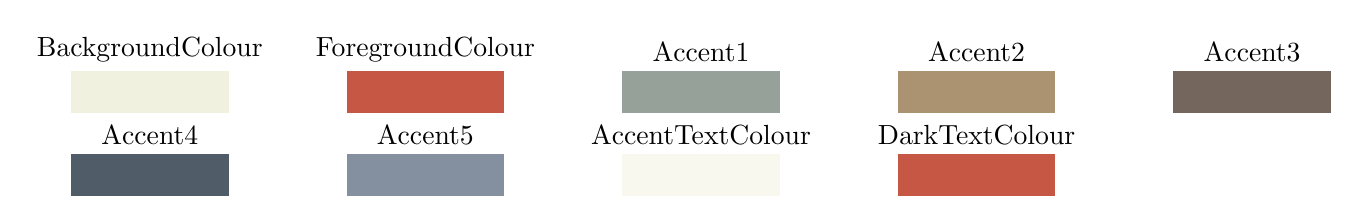
\begin{tikzpicture}
\definecolor{col}{HTML}{F0F1DF}
\fill[col] (0.0, -0.5em + 0em) rectangle (2.0, 1em + 0em) (1.0, 1em + 0em) node[above, text = black] {BackgroundColour};
\definecolor{col}{HTML}{C65744}
\fill[col] (3.5, -0.5em + 0em) rectangle (5.5, 1em + 0em) (4.5, 1em + 0em) node[above, text = black] {ForegroundColour};
\definecolor{col}{HTML}{96A199}
\fill[col] (7.0, -0.5em + 0em) rectangle (9.0, 1em + 0em) (8.0, 1em + 0em) node[above, text = black] {Accent1};
\definecolor{col}{HTML}{AB9371}
\fill[col] (10.5, -0.5em + 0em) rectangle (12.5, 1em + 0em) (11.5, 1em + 0em) node[above, text = black] {Accent2};
\definecolor{col}{HTML}{74665D}
\fill[col] (14.0, -0.5em + 0em) rectangle (16.0, 1em + 0em) (15.0, 1em + 0em) node[above, text = black] {Accent3};
\definecolor{col}{HTML}{505C68}
\fill[col] (0.0, -0.5em + -3em) rectangle (2.0, 1em + -3em) (1.0, 1em + -3em) node[above, text = black] {Accent4};
\definecolor{col}{HTML}{8490A0}
\fill[col] (3.5, -0.5em + -3em) rectangle (5.5, 1em + -3em) (4.5, 1em + -3em) node[above, text = black] {Accent5};
\definecolor{col}{HTML}{F0F1DF}
\fill[col!50!white] (7.0, -0.5em + -3em) rectangle (9.0, 1em + -3em) (8.0, 1em + -3em) node[above, text = black] {AccentTextColour};
\definecolor{col}{HTML}{C65744}
\fill[col] (10.5, -0.5em + -3em) rectangle (12.5, 1em + -3em) (11.5, 1em + -3em) node[above, text = black] {DarkTextColour};
\end{tikzpicture}

\subsection*{Couture}
\subsubsection*{Light}
\noindent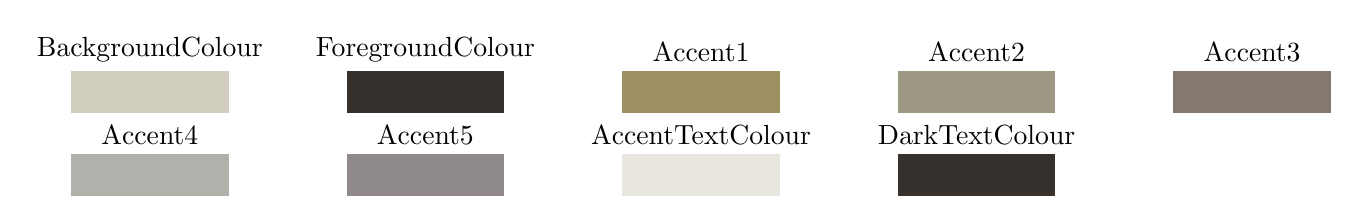
\begin{tikzpicture}
\definecolor{col}{HTML}{D1CEBF}
\fill[col] (0.0, -0.5em + 0em) rectangle (2.0, 1em + 0em) (1.0, 1em + 0em) node[above, text = black] {BackgroundColour};
\definecolor{col}{HTML}{36312D}
\fill[col] (3.5, -0.5em + 0em) rectangle (5.5, 1em + 0em) (4.5, 1em + 0em) node[above, text = black] {ForegroundColour};
\definecolor{col}{HTML}{9E9063}
\fill[col] (7.0, -0.5em + 0em) rectangle (9.0, 1em + 0em) (8.0, 1em + 0em) node[above, text = black] {Accent1};
\definecolor{col}{HTML}{9E9985}
\fill[col] (10.5, -0.5em + 0em) rectangle (12.5, 1em + 0em) (11.5, 1em + 0em) node[above, text = black] {Accent2};
\definecolor{col}{HTML}{85786F}
\fill[col] (14.0, -0.5em + 0em) rectangle (16.0, 1em + 0em) (15.0, 1em + 0em) node[above, text = black] {Accent3};
\definecolor{col}{HTML}{B0B1AB}
\fill[col] (0.0, -0.5em + -3em) rectangle (2.0, 1em + -3em) (1.0, 1em + -3em) node[above, text = black] {Accent4};
\definecolor{col}{HTML}{8F898D}
\fill[col] (3.5, -0.5em + -3em) rectangle (5.5, 1em + -3em) (4.5, 1em + -3em) node[above, text = black] {Accent5};
\definecolor{col}{HTML}{D1CEBF}
\fill[col!50!white] (7.0, -0.5em + -3em) rectangle (9.0, 1em + -3em) (8.0, 1em + -3em) node[above, text = black] {AccentTextColour};
\definecolor{col}{HTML}{36312D}
\fill[col] (10.5, -0.5em + -3em) rectangle (12.5, 1em + -3em) (11.5, 1em + -3em) node[above, text = black] {DarkTextColour};
\end{tikzpicture}

\subsection*{Elemental}
\subsubsection*{Light}
\noindent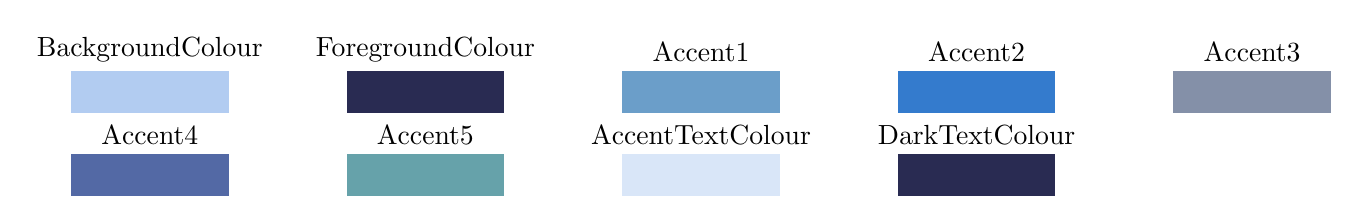
\begin{tikzpicture}
\definecolor{col}{HTML}{B2CCF1}
\fill[col] (0.0, -0.5em + 0em) rectangle (2.0, 1em + 0em) (1.0, 1em + 0em) node[above, text = black] {BackgroundColour};
\definecolor{col}{HTML}{292B52}
\fill[col] (3.5, -0.5em + 0em) rectangle (5.5, 1em + 0em) (4.5, 1em + 0em) node[above, text = black] {ForegroundColour};
\definecolor{col}{HTML}{6B9EC9}
\fill[col] (7.0, -0.5em + 0em) rectangle (9.0, 1em + 0em) (8.0, 1em + 0em) node[above, text = black] {Accent1};
\definecolor{col}{HTML}{347BCD}
\fill[col] (10.5, -0.5em + 0em) rectangle (12.5, 1em + 0em) (11.5, 1em + 0em) node[above, text = black] {Accent2};
\definecolor{col}{HTML}{8490A8}
\fill[col] (14.0, -0.5em + 0em) rectangle (16.0, 1em + 0em) (15.0, 1em + 0em) node[above, text = black] {Accent3};
\definecolor{col}{HTML}{5369A5}
\fill[col] (0.0, -0.5em + -3em) rectangle (2.0, 1em + -3em) (1.0, 1em + -3em) node[above, text = black] {Accent4};
\definecolor{col}{HTML}{66A2AA}
\fill[col] (3.5, -0.5em + -3em) rectangle (5.5, 1em + -3em) (4.5, 1em + -3em) node[above, text = black] {Accent5};
\definecolor{col}{HTML}{B2CCF1}
\fill[col!50!white] (7.0, -0.5em + -3em) rectangle (9.0, 1em + -3em) (8.0, 1em + -3em) node[above, text = black] {AccentTextColour};
\definecolor{col}{HTML}{292B52}
\fill[col] (10.5, -0.5em + -3em) rectangle (12.5, 1em + -3em) (11.5, 1em + -3em) node[above, text = black] {DarkTextColour};
\end{tikzpicture}

\subsection*{Essential}
\subsubsection*{Light}
\noindent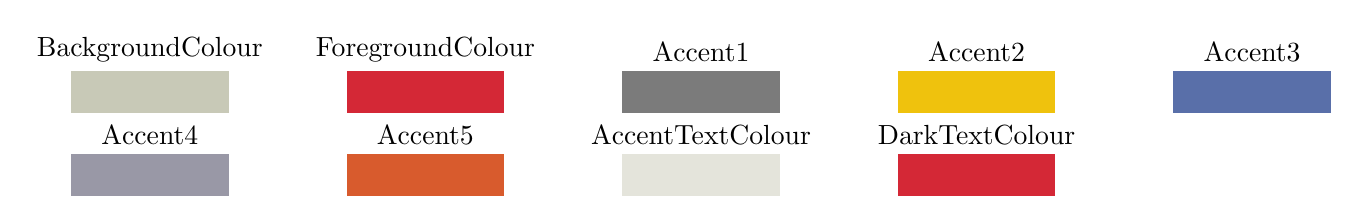
\begin{tikzpicture}
\definecolor{col}{HTML}{C8C9B7}
\fill[col] (0.0, -0.5em + 0em) rectangle (2.0, 1em + 0em) (1.0, 1em + 0em) node[above, text = black] {BackgroundColour};
\definecolor{col}{HTML}{D42836}
\fill[col] (3.5, -0.5em + 0em) rectangle (5.5, 1em + 0em) (4.5, 1em + 0em) node[above, text = black] {ForegroundColour};
\definecolor{col}{HTML}{7B7B7B}
\fill[col] (7.0, -0.5em + 0em) rectangle (9.0, 1em + 0em) (8.0, 1em + 0em) node[above, text = black] {Accent1};
\definecolor{col}{HTML}{EFC20D}
\fill[col] (10.5, -0.5em + 0em) rectangle (12.5, 1em + 0em) (11.5, 1em + 0em) node[above, text = black] {Accent2};
\definecolor{col}{HTML}{596FA9}
\fill[col] (14.0, -0.5em + 0em) rectangle (16.0, 1em + 0em) (15.0, 1em + 0em) node[above, text = black] {Accent3};
\definecolor{col}{HTML}{9998A6}
\fill[col] (0.0, -0.5em + -3em) rectangle (2.0, 1em + -3em) (1.0, 1em + -3em) node[above, text = black] {Accent4};
\definecolor{col}{HTML}{D85B2D}
\fill[col] (3.5, -0.5em + -3em) rectangle (5.5, 1em + -3em) (4.5, 1em + -3em) node[above, text = black] {Accent5};
\definecolor{col}{HTML}{C8C9B7}
\fill[col!50!white] (7.0, -0.5em + -3em) rectangle (9.0, 1em + -3em) (8.0, 1em + -3em) node[above, text = black] {AccentTextColour};
\definecolor{col}{HTML}{D42836}
\fill[col] (10.5, -0.5em + -3em) rectangle (12.5, 1em + -3em) (11.5, 1em + -3em) node[above, text = black] {DarkTextColour};
\end{tikzpicture}

\subsection*{Executive}
\subsubsection*{Light}
\noindent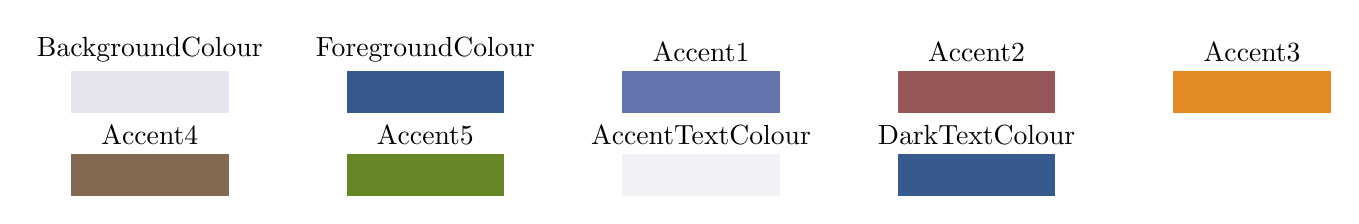
\begin{tikzpicture}
\definecolor{col}{HTML}{E5E5ED}
\fill[col] (0.0, -0.5em + 0em) rectangle (2.0, 1em + 0em) (1.0, 1em + 0em) node[above, text = black] {BackgroundColour};
\definecolor{col}{HTML}{365A8E}
\fill[col] (3.5, -0.5em + 0em) rectangle (5.5, 1em + 0em) (4.5, 1em + 0em) node[above, text = black] {ForegroundColour};
\definecolor{col}{HTML}{6574AD}
\fill[col] (7.0, -0.5em + 0em) rectangle (9.0, 1em + 0em) (8.0, 1em + 0em) node[above, text = black] {Accent1};
\definecolor{col}{HTML}{955758}
\fill[col] (10.5, -0.5em + 0em) rectangle (12.5, 1em + 0em) (11.5, 1em + 0em) node[above, text = black] {Accent2};
\definecolor{col}{HTML}{E28B24}
\fill[col] (14.0, -0.5em + 0em) rectangle (16.0, 1em + 0em) (15.0, 1em + 0em) node[above, text = black] {Accent3};
\definecolor{col}{HTML}{836952}
\fill[col] (0.0, -0.5em + -3em) rectangle (2.0, 1em + -3em) (1.0, 1em + -3em) node[above, text = black] {Accent4};
\definecolor{col}{HTML}{678726}
\fill[col] (3.5, -0.5em + -3em) rectangle (5.5, 1em + -3em) (4.5, 1em + -3em) node[above, text = black] {Accent5};
\definecolor{col}{HTML}{E5E5ED}
\fill[col!50!white] (7.0, -0.5em + -3em) rectangle (9.0, 1em + -3em) (8.0, 1em + -3em) node[above, text = black] {AccentTextColour};
\definecolor{col}{HTML}{365A8E}
\fill[col] (10.5, -0.5em + -3em) rectangle (12.5, 1em + -3em) (11.5, 1em + -3em) node[above, text = black] {DarkTextColour};
\end{tikzpicture}

\subsection*{Expo}
\subsubsection*{Light}
\noindent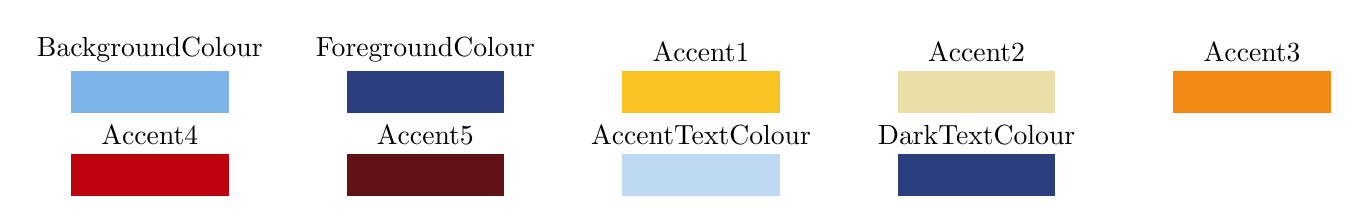
\begin{tikzpicture}
\definecolor{col}{HTML}{7CB4E7}
\fill[col] (0.0, -0.5em + 0em) rectangle (2.0, 1em + 0em) (1.0, 1em + 0em) node[above, text = black] {BackgroundColour};
\definecolor{col}{HTML}{2B3D7D}
\fill[col] (3.5, -0.5em + 0em) rectangle (5.5, 1em + 0em) (4.5, 1em + 0em) node[above, text = black] {ForegroundColour};
\definecolor{col}{HTML}{F8C222}
\fill[col] (7.0, -0.5em + 0em) rectangle (9.0, 1em + 0em) (8.0, 1em + 0em) node[above, text = black] {Accent1};
\definecolor{col}{HTML}{EADFA9}
\fill[col] (10.5, -0.5em + 0em) rectangle (12.5, 1em + 0em) (11.5, 1em + 0em) node[above, text = black] {Accent2};
\definecolor{col}{HTML}{F28914}
\fill[col] (14.0, -0.5em + 0em) rectangle (16.0, 1em + 0em) (15.0, 1em + 0em) node[above, text = black] {Accent3};
\definecolor{col}{HTML}{BD030E}
\fill[col] (0.0, -0.5em + -3em) rectangle (2.0, 1em + -3em) (1.0, 1em + -3em) node[above, text = black] {Accent4};
\definecolor{col}{HTML}{621215}
\fill[col] (3.5, -0.5em + -3em) rectangle (5.5, 1em + -3em) (4.5, 1em + -3em) node[above, text = black] {Accent5};
\definecolor{col}{HTML}{7CB4E7}
\fill[col!50!white] (7.0, -0.5em + -3em) rectangle (9.0, 1em + -3em) (8.0, 1em + -3em) node[above, text = black] {AccentTextColour};
\definecolor{col}{HTML}{2B3D7D}
\fill[col] (10.5, -0.5em + -3em) rectangle (12.5, 1em + -3em) (11.5, 1em + -3em) node[above, text = black] {DarkTextColour};
\end{tikzpicture}

\subsection*{Folio}
\subsubsection*{Light}
\noindent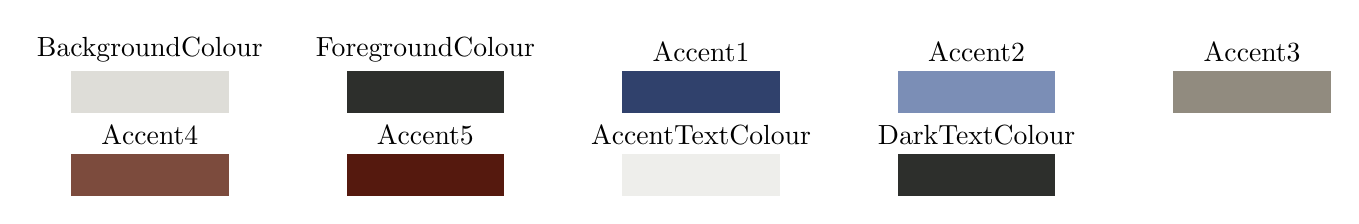
\begin{tikzpicture}
\definecolor{col}{HTML}{DEDDD8}
\fill[col] (0.0, -0.5em + 0em) rectangle (2.0, 1em + 0em) (1.0, 1em + 0em) node[above, text = black] {BackgroundColour};
\definecolor{col}{HTML}{2D2F2C}
\fill[col] (3.5, -0.5em + 0em) rectangle (5.5, 1em + 0em) (4.5, 1em + 0em) node[above, text = black] {ForegroundColour};
\definecolor{col}{HTML}{30416C}
\fill[col] (7.0, -0.5em + 0em) rectangle (9.0, 1em + 0em) (8.0, 1em + 0em) node[above, text = black] {Accent1};
\definecolor{col}{HTML}{7B8EB6}
\fill[col] (10.5, -0.5em + 0em) rectangle (12.5, 1em + 0em) (11.5, 1em + 0em) node[above, text = black] {Accent2};
\definecolor{col}{HTML}{918B7F}
\fill[col] (14.0, -0.5em + 0em) rectangle (16.0, 1em + 0em) (15.0, 1em + 0em) node[above, text = black] {Accent3};
\definecolor{col}{HTML}{7C4B3D}
\fill[col] (0.0, -0.5em + -3em) rectangle (2.0, 1em + -3em) (1.0, 1em + -3em) node[above, text = black] {Accent4};
\definecolor{col}{HTML}{55190E}
\fill[col] (3.5, -0.5em + -3em) rectangle (5.5, 1em + -3em) (4.5, 1em + -3em) node[above, text = black] {Accent5};
\definecolor{col}{HTML}{DEDDD8}
\fill[col!50!white] (7.0, -0.5em + -3em) rectangle (9.0, 1em + -3em) (8.0, 1em + -3em) node[above, text = black] {AccentTextColour};
\definecolor{col}{HTML}{2D2F2C}
\fill[col] (10.5, -0.5em + -3em) rectangle (12.5, 1em + -3em) (11.5, 1em + -3em) node[above, text = black] {DarkTextColour};
\end{tikzpicture}

\subsection*{Formal}
\subsubsection*{Light}
\noindent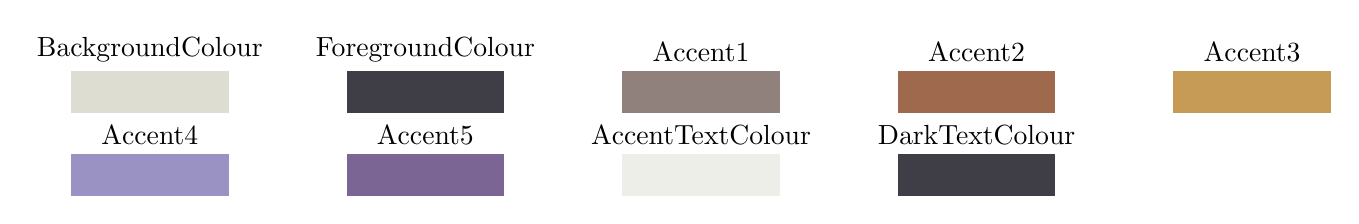
\begin{tikzpicture}
\definecolor{col}{HTML}{DDDDD1}
\fill[col] (0.0, -0.5em + 0em) rectangle (2.0, 1em + 0em) (1.0, 1em + 0em) node[above, text = black] {BackgroundColour};
\definecolor{col}{HTML}{3F3E46}
\fill[col] (3.5, -0.5em + 0em) rectangle (5.5, 1em + 0em) (4.5, 1em + 0em) node[above, text = black] {ForegroundColour};
\definecolor{col}{HTML}{90817C}
\fill[col] (7.0, -0.5em + 0em) rectangle (9.0, 1em + 0em) (8.0, 1em + 0em) node[above, text = black] {Accent1};
\definecolor{col}{HTML}{9F694D}
\fill[col] (10.5, -0.5em + 0em) rectangle (12.5, 1em + 0em) (11.5, 1em + 0em) node[above, text = black] {Accent2};
\definecolor{col}{HTML}{C69B56}
\fill[col] (14.0, -0.5em + 0em) rectangle (16.0, 1em + 0em) (15.0, 1em + 0em) node[above, text = black] {Accent3};
\definecolor{col}{HTML}{9A92C3}
\fill[col] (0.0, -0.5em + -3em) rectangle (2.0, 1em + -3em) (1.0, 1em + -3em) node[above, text = black] {Accent4};
\definecolor{col}{HTML}{7B6594}
\fill[col] (3.5, -0.5em + -3em) rectangle (5.5, 1em + -3em) (4.5, 1em + -3em) node[above, text = black] {Accent5};
\definecolor{col}{HTML}{DDDDD1}
\fill[col!50!white] (7.0, -0.5em + -3em) rectangle (9.0, 1em + -3em) (8.0, 1em + -3em) node[above, text = black] {AccentTextColour};
\definecolor{col}{HTML}{3F3E46}
\fill[col] (10.5, -0.5em + -3em) rectangle (12.5, 1em + -3em) (11.5, 1em + -3em) node[above, text = black] {DarkTextColour};
\end{tikzpicture}

\subsection*{Foundry}
\subsubsection*{Light}
\noindent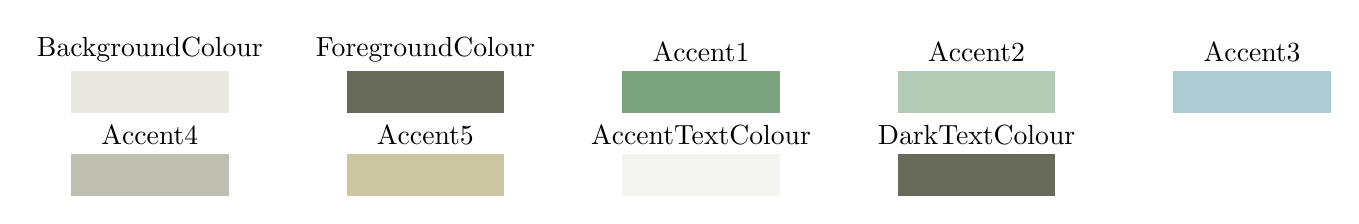
\begin{tikzpicture}
\definecolor{col}{HTML}{E9E9E1}
\fill[col] (0.0, -0.5em + 0em) rectangle (2.0, 1em + 0em) (1.0, 1em + 0em) node[above, text = black] {BackgroundColour};
\definecolor{col}{HTML}{676A59}
\fill[col] (3.5, -0.5em + 0em) rectangle (5.5, 1em + 0em) (4.5, 1em + 0em) node[above, text = black] {ForegroundColour};
\definecolor{col}{HTML}{7BA37E}
\fill[col] (7.0, -0.5em + 0em) rectangle (9.0, 1em + 0em) (8.0, 1em + 0em) node[above, text = black] {Accent1};
\definecolor{col}{HTML}{B3CBB5}
\fill[col] (10.5, -0.5em + 0em) rectangle (12.5, 1em + 0em) (11.5, 1em + 0em) node[above, text = black] {Accent2};
\definecolor{col}{HTML}{ADCBD3}
\fill[col] (14.0, -0.5em + 0em) rectangle (16.0, 1em + 0em) (15.0, 1em + 0em) node[above, text = black] {Accent3};
\definecolor{col}{HTML}{BEBFB1}
\fill[col] (0.0, -0.5em + -3em) rectangle (2.0, 1em + -3em) (1.0, 1em + -3em) node[above, text = black] {Accent4};
\definecolor{col}{HTML}{CBC6A0}
\fill[col] (3.5, -0.5em + -3em) rectangle (5.5, 1em + -3em) (4.5, 1em + -3em) node[above, text = black] {Accent5};
\definecolor{col}{HTML}{E9E9E1}
\fill[col!50!white] (7.0, -0.5em + -3em) rectangle (9.0, 1em + -3em) (8.0, 1em + -3em) node[above, text = black] {AccentTextColour};
\definecolor{col}{HTML}{676A59}
\fill[col] (10.5, -0.5em + -3em) rectangle (12.5, 1em + -3em) (11.5, 1em + -3em) node[above, text = black] {DarkTextColour};
\end{tikzpicture}

\subsection*{Genesis}
\subsubsection*{Light}
\noindent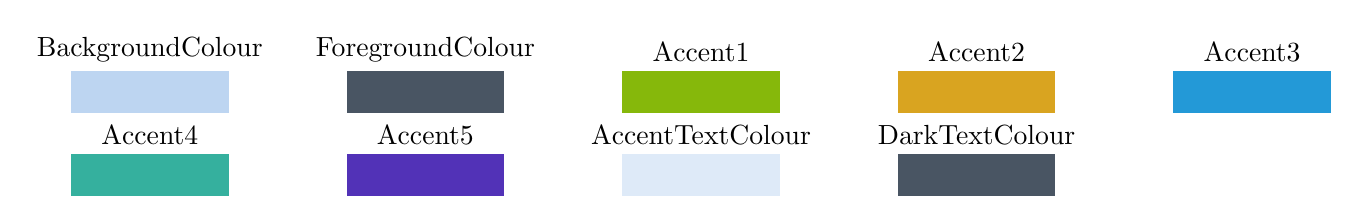
\begin{tikzpicture}
\definecolor{col}{HTML}{BDD5F1}
\fill[col] (0.0, -0.5em + 0em) rectangle (2.0, 1em + 0em) (1.0, 1em + 0em) node[above, text = black] {BackgroundColour};
\definecolor{col}{HTML}{495563}
\fill[col] (3.5, -0.5em + 0em) rectangle (5.5, 1em + 0em) (4.5, 1em + 0em) node[above, text = black] {ForegroundColour};
\definecolor{col}{HTML}{86B80B}
\fill[col] (7.0, -0.5em + 0em) rectangle (9.0, 1em + 0em) (8.0, 1em + 0em) node[above, text = black] {Accent1};
\definecolor{col}{HTML}{D9A420}
\fill[col] (10.5, -0.5em + 0em) rectangle (12.5, 1em + 0em) (11.5, 1em + 0em) node[above, text = black] {Accent2};
\definecolor{col}{HTML}{2399D7}
\fill[col] (14.0, -0.5em + 0em) rectangle (16.0, 1em + 0em) (15.0, 1em + 0em) node[above, text = black] {Accent3};
\definecolor{col}{HTML}{35B09E}
\fill[col] (0.0, -0.5em + -3em) rectangle (2.0, 1em + -3em) (1.0, 1em + -3em) node[above, text = black] {Accent4};
\definecolor{col}{HTML}{5232B7}
\fill[col] (3.5, -0.5em + -3em) rectangle (5.5, 1em + -3em) (4.5, 1em + -3em) node[above, text = black] {Accent5};
\definecolor{col}{HTML}{BDD5F1}
\fill[col!50!white] (7.0, -0.5em + -3em) rectangle (9.0, 1em + -3em) (8.0, 1em + -3em) node[above, text = black] {AccentTextColour};
\definecolor{col}{HTML}{495563}
\fill[col] (10.5, -0.5em + -3em) rectangle (12.5, 1em + -3em) (11.5, 1em + -3em) node[above, text = black] {DarkTextColour};
\end{tikzpicture}

\subsection*{Grid}
\subsubsection*{Light}
\noindent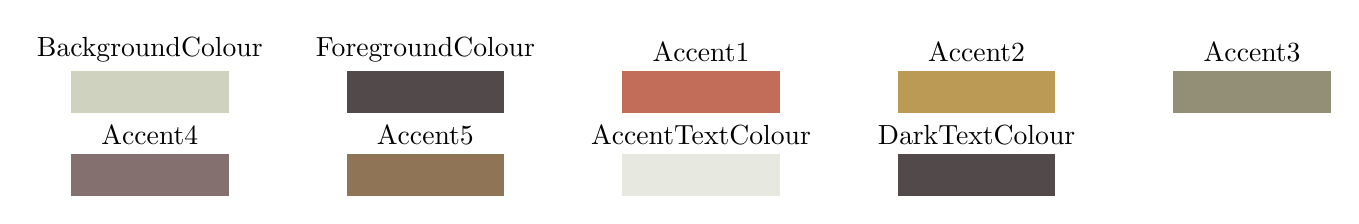
\begin{tikzpicture}
\definecolor{col}{HTML}{CFD2BF}
\fill[col] (0.0, -0.5em + 0em) rectangle (2.0, 1em + 0em) (1.0, 1em + 0em) node[above, text = black] {BackgroundColour};
\definecolor{col}{HTML}{52494A}
\fill[col] (3.5, -0.5em + 0em) rectangle (5.5, 1em + 0em) (4.5, 1em + 0em) node[above, text = black] {ForegroundColour};
\definecolor{col}{HTML}{C26D59}
\fill[col] (7.0, -0.5em + 0em) rectangle (9.0, 1em + 0em) (8.0, 1em + 0em) node[above, text = black] {Accent1};
\definecolor{col}{HTML}{BB9A55}
\fill[col] (10.5, -0.5em + 0em) rectangle (12.5, 1em + 0em) (11.5, 1em + 0em) node[above, text = black] {Accent2};
\definecolor{col}{HTML}{938F76}
\fill[col] (14.0, -0.5em + 0em) rectangle (16.0, 1em + 0em) (15.0, 1em + 0em) node[above, text = black] {Accent3};
\definecolor{col}{HTML}{84706F}
\fill[col] (0.0, -0.5em + -3em) rectangle (2.0, 1em + -3em) (1.0, 1em + -3em) node[above, text = black] {Accent4};
\definecolor{col}{HTML}{8F7456}
\fill[col] (3.5, -0.5em + -3em) rectangle (5.5, 1em + -3em) (4.5, 1em + -3em) node[above, text = black] {Accent5};
\definecolor{col}{HTML}{CFD2BF}
\fill[col!50!white] (7.0, -0.5em + -3em) rectangle (9.0, 1em + -3em) (8.0, 1em + -3em) node[above, text = black] {AccentTextColour};
\definecolor{col}{HTML}{52494A}
\fill[col] (10.5, -0.5em + -3em) rectangle (12.5, 1em + -3em) (11.5, 1em + -3em) node[above, text = black] {DarkTextColour};
\end{tikzpicture}

\subsection*{Habitat}
\subsubsection*{Light}
\noindent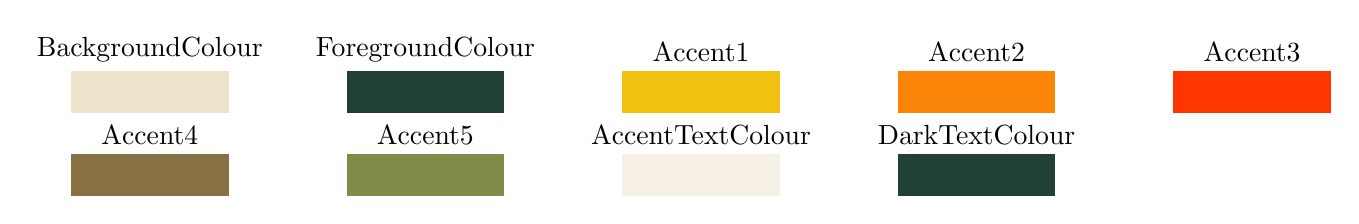
\begin{tikzpicture}
\definecolor{col}{HTML}{EDE3CA}
\fill[col] (0.0, -0.5em + 0em) rectangle (2.0, 1em + 0em) (1.0, 1em + 0em) node[above, text = black] {BackgroundColour};
\definecolor{col}{HTML}{214134}
\fill[col] (3.5, -0.5em + 0em) rectangle (5.5, 1em + 0em) (4.5, 1em + 0em) node[above, text = black] {ForegroundColour};
\definecolor{col}{HTML}{F0C10F}
\fill[col] (7.0, -0.5em + 0em) rectangle (9.0, 1em + 0em) (8.0, 1em + 0em) node[above, text = black] {Accent1};
\definecolor{col}{HTML}{FB8509}
\fill[col] (10.5, -0.5em + 0em) rectangle (12.5, 1em + 0em) (11.5, 1em + 0em) node[above, text = black] {Accent2};
\definecolor{col}{HTML}{FF3602}
\fill[col] (14.0, -0.5em + 0em) rectangle (16.0, 1em + 0em) (15.0, 1em + 0em) node[above, text = black] {Accent3};
\definecolor{col}{HTML}{887145}
\fill[col] (0.0, -0.5em + -3em) rectangle (2.0, 1em + -3em) (1.0, 1em + -3em) node[above, text = black] {Accent4};
\definecolor{col}{HTML}{828B4A}
\fill[col] (3.5, -0.5em + -3em) rectangle (5.5, 1em + -3em) (4.5, 1em + -3em) node[above, text = black] {Accent5};
\definecolor{col}{HTML}{EDE3CA}
\fill[col!50!white] (7.0, -0.5em + -3em) rectangle (9.0, 1em + -3em) (8.0, 1em + -3em) node[above, text = black] {AccentTextColour};
\definecolor{col}{HTML}{214134}
\fill[col] (10.5, -0.5em + -3em) rectangle (12.5, 1em + -3em) (11.5, 1em + -3em) node[above, text = black] {DarkTextColour};
\end{tikzpicture}

\subsection*{Hardcover}
\subsubsection*{Light}
\noindent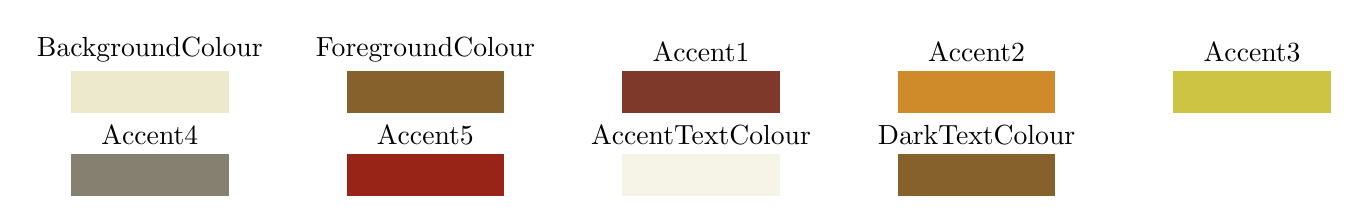
\begin{tikzpicture}
\definecolor{col}{HTML}{EDE9CC}
\fill[col] (0.0, -0.5em + 0em) rectangle (2.0, 1em + 0em) (1.0, 1em + 0em) node[above, text = black] {BackgroundColour};
\definecolor{col}{HTML}{86612C}
\fill[col] (3.5, -0.5em + 0em) rectangle (5.5, 1em + 0em) (4.5, 1em + 0em) node[above, text = black] {ForegroundColour};
\definecolor{col}{HTML}{7E392A}
\fill[col] (7.0, -0.5em + 0em) rectangle (9.0, 1em + 0em) (8.0, 1em + 0em) node[above, text = black] {Accent1};
\definecolor{col}{HTML}{CF8B2A}
\fill[col] (10.5, -0.5em + 0em) rectangle (12.5, 1em + 0em) (11.5, 1em + 0em) node[above, text = black] {Accent2};
\definecolor{col}{HTML}{CDC443}
\fill[col] (14.0, -0.5em + 0em) rectangle (16.0, 1em + 0em) (15.0, 1em + 0em) node[above, text = black] {Accent3};
\definecolor{col}{HTML}{868070}
\fill[col] (0.0, -0.5em + -3em) rectangle (2.0, 1em + -3em) (1.0, 1em + -3em) node[above, text = black] {Accent4};
\definecolor{col}{HTML}{982417}
\fill[col] (3.5, -0.5em + -3em) rectangle (5.5, 1em + -3em) (4.5, 1em + -3em) node[above, text = black] {Accent5};
\definecolor{col}{HTML}{EDE9CC}
\fill[col!50!white] (7.0, -0.5em + -3em) rectangle (9.0, 1em + -3em) (8.0, 1em + -3em) node[above, text = black] {AccentTextColour};
\definecolor{col}{HTML}{86612C}
\fill[col] (10.5, -0.5em + -3em) rectangle (12.5, 1em + -3em) (11.5, 1em + -3em) node[above, text = black] {DarkTextColour};
\end{tikzpicture}

\subsection*{Horizon}
\subsubsection*{Light}
\noindent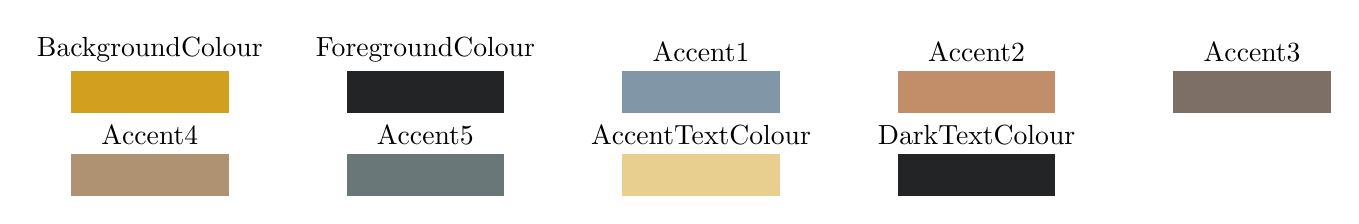
\begin{tikzpicture}
\definecolor{col}{HTML}{D29F1F}
\fill[col] (0.0, -0.5em + 0em) rectangle (2.0, 1em + 0em) (1.0, 1em + 0em) node[above, text = black] {BackgroundColour};
\definecolor{col}{HTML}{232426}
\fill[col] (3.5, -0.5em + 0em) rectangle (5.5, 1em + 0em) (4.5, 1em + 0em) node[above, text = black] {ForegroundColour};
\definecolor{col}{HTML}{8196A7}
\fill[col] (7.0, -0.5em + 0em) rectangle (9.0, 1em + 0em) (8.0, 1em + 0em) node[above, text = black] {Accent1};
\definecolor{col}{HTML}{C28E69}
\fill[col] (10.5, -0.5em + 0em) rectangle (12.5, 1em + 0em) (11.5, 1em + 0em) node[above, text = black] {Accent2};
\definecolor{col}{HTML}{7D6F66}
\fill[col] (14.0, -0.5em + 0em) rectangle (16.0, 1em + 0em) (15.0, 1em + 0em) node[above, text = black] {Accent3};
\definecolor{col}{HTML}{AF9272}
\fill[col] (0.0, -0.5em + -3em) rectangle (2.0, 1em + -3em) (1.0, 1em + -3em) node[above, text = black] {Accent4};
\definecolor{col}{HTML}{697778}
\fill[col] (3.5, -0.5em + -3em) rectangle (5.5, 1em + -3em) (4.5, 1em + -3em) node[above, text = black] {Accent5};
\definecolor{col}{HTML}{D29F1F}
\fill[col!50!white] (7.0, -0.5em + -3em) rectangle (9.0, 1em + -3em) (8.0, 1em + -3em) node[above, text = black] {AccentTextColour};
\definecolor{col}{HTML}{232426}
\fill[col] (10.5, -0.5em + -3em) rectangle (12.5, 1em + -3em) (11.5, 1em + -3em) node[above, text = black] {DarkTextColour};
\end{tikzpicture}

\subsection*{Infusion}
\subsubsection*{Light}
\noindent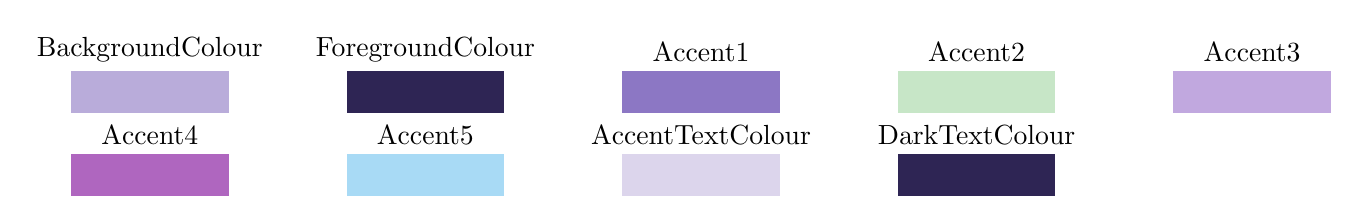
\begin{tikzpicture}
\definecolor{col}{HTML}{B9ACDA}
\fill[col] (0.0, -0.5em + 0em) rectangle (2.0, 1em + 0em) (1.0, 1em + 0em) node[above, text = black] {BackgroundColour};
\definecolor{col}{HTML}{2E2554}
\fill[col] (3.5, -0.5em + 0em) rectangle (5.5, 1em + 0em) (4.5, 1em + 0em) node[above, text = black] {ForegroundColour};
\definecolor{col}{HTML}{8C77C4}
\fill[col] (7.0, -0.5em + 0em) rectangle (9.0, 1em + 0em) (8.0, 1em + 0em) node[above, text = black] {Accent1};
\definecolor{col}{HTML}{C7E6C7}
\fill[col] (10.5, -0.5em + 0em) rectangle (12.5, 1em + 0em) (11.5, 1em + 0em) node[above, text = black] {Accent2};
\definecolor{col}{HTML}{C1A8DF}
\fill[col] (14.0, -0.5em + 0em) rectangle (16.0, 1em + 0em) (15.0, 1em + 0em) node[above, text = black] {Accent3};
\definecolor{col}{HTML}{AF66BF}
\fill[col] (0.0, -0.5em + -3em) rectangle (2.0, 1em + -3em) (1.0, 1em + -3em) node[above, text = black] {Accent4};
\definecolor{col}{HTML}{A8DAF5}
\fill[col] (3.5, -0.5em + -3em) rectangle (5.5, 1em + -3em) (4.5, 1em + -3em) node[above, text = black] {Accent5};
\definecolor{col}{HTML}{B9ACDA}
\fill[col!50!white] (7.0, -0.5em + -3em) rectangle (9.0, 1em + -3em) (8.0, 1em + -3em) node[above, text = black] {AccentTextColour};
\definecolor{col}{HTML}{2E2554}
\fill[col] (10.5, -0.5em + -3em) rectangle (12.5, 1em + -3em) (11.5, 1em + -3em) node[above, text = black] {DarkTextColour};
\end{tikzpicture}

\subsection*{Inkwell}
\subsubsection*{Light}
\noindent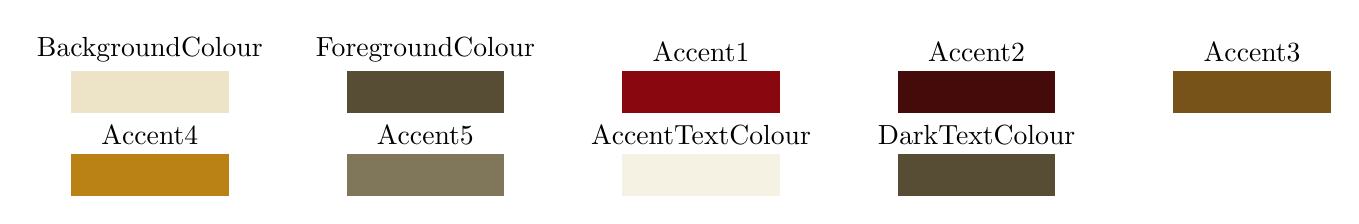
\begin{tikzpicture}
\definecolor{col}{HTML}{EDE4C7}
\fill[col] (0.0, -0.5em + 0em) rectangle (2.0, 1em + 0em) (1.0, 1em + 0em) node[above, text = black] {BackgroundColour};
\definecolor{col}{HTML}{574D34}
\fill[col] (3.5, -0.5em + 0em) rectangle (5.5, 1em + 0em) (4.5, 1em + 0em) node[above, text = black] {ForegroundColour};
\definecolor{col}{HTML}{89070F}
\fill[col] (7.0, -0.5em + 0em) rectangle (9.0, 1em + 0em) (8.0, 1em + 0em) node[above, text = black] {Accent1};
\definecolor{col}{HTML}{450B0A}
\fill[col] (10.5, -0.5em + 0em) rectangle (12.5, 1em + 0em) (11.5, 1em + 0em) node[above, text = black] {Accent2};
\definecolor{col}{HTML}{775319}
\fill[col] (14.0, -0.5em + 0em) rectangle (16.0, 1em + 0em) (15.0, 1em + 0em) node[above, text = black] {Accent3};
\definecolor{col}{HTML}{BA8215}
\fill[col] (0.0, -0.5em + -3em) rectangle (2.0, 1em + -3em) (1.0, 1em + -3em) node[above, text = black] {Accent4};
\definecolor{col}{HTML}{80775A}
\fill[col] (3.5, -0.5em + -3em) rectangle (5.5, 1em + -3em) (4.5, 1em + -3em) node[above, text = black] {Accent5};
\definecolor{col}{HTML}{EDE4C7}
\fill[col!50!white] (7.0, -0.5em + -3em) rectangle (9.0, 1em + -3em) (8.0, 1em + -3em) node[above, text = black] {AccentTextColour};
\definecolor{col}{HTML}{574D34}
\fill[col] (10.5, -0.5em + -3em) rectangle (12.5, 1em + -3em) (11.5, 1em + -3em) node[above, text = black] {DarkTextColour};
\end{tikzpicture}

\subsection*{Median}
\subsubsection*{Light}
\noindent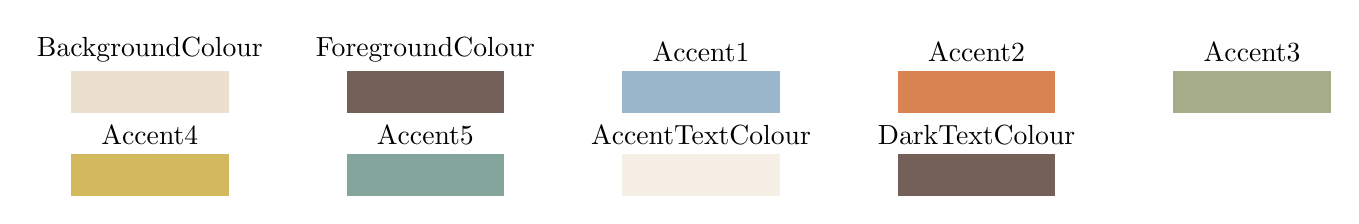
\begin{tikzpicture}
\definecolor{col}{HTML}{EBE0CE}
\fill[col] (0.0, -0.5em + 0em) rectangle (2.0, 1em + 0em) (1.0, 1em + 0em) node[above, text = black] {BackgroundColour};
\definecolor{col}{HTML}{746059}
\fill[col] (3.5, -0.5em + 0em) rectangle (5.5, 1em + 0em) (4.5, 1em + 0em) node[above, text = black] {ForegroundColour};
\definecolor{col}{HTML}{9AB6CB}
\fill[col] (7.0, -0.5em + 0em) rectangle (9.0, 1em + 0em) (8.0, 1em + 0em) node[above, text = black] {Accent1};
\definecolor{col}{HTML}{D98352}
\fill[col] (10.5, -0.5em + 0em) rectangle (12.5, 1em + 0em) (11.5, 1em + 0em) node[above, text = black] {Accent2};
\definecolor{col}{HTML}{A6AC88}
\fill[col] (14.0, -0.5em + 0em) rectangle (16.0, 1em + 0em) (15.0, 1em + 0em) node[above, text = black] {Accent3};
\definecolor{col}{HTML}{D3B85D}
\fill[col] (0.0, -0.5em + -3em) rectangle (2.0, 1em + -3em) (1.0, 1em + -3em) node[above, text = black] {Accent4};
\definecolor{col}{HTML}{84A59C}
\fill[col] (3.5, -0.5em + -3em) rectangle (5.5, 1em + -3em) (4.5, 1em + -3em) node[above, text = black] {Accent5};
\definecolor{col}{HTML}{EBE0CE}
\fill[col!50!white] (7.0, -0.5em + -3em) rectangle (9.0, 1em + -3em) (8.0, 1em + -3em) node[above, text = black] {AccentTextColour};
\definecolor{col}{HTML}{746059}
\fill[col] (10.5, -0.5em + -3em) rectangle (12.5, 1em + -3em) (11.5, 1em + -3em) node[above, text = black] {DarkTextColour};
\end{tikzpicture}

\subsection*{Kilter}
\subsubsection*{Light}
\noindent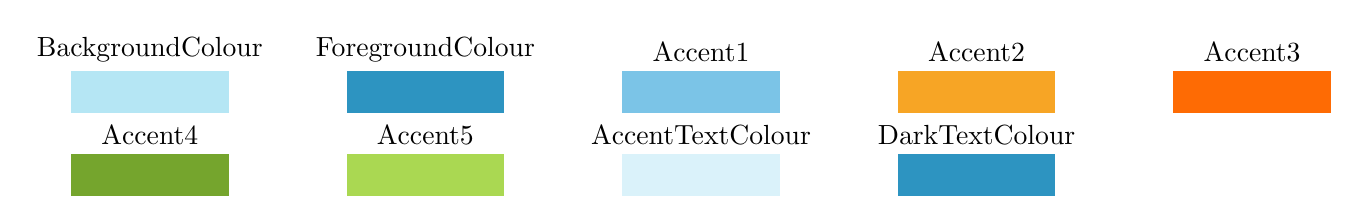
\begin{tikzpicture}
\definecolor{col}{HTML}{B5E6F4}
\fill[col] (0.0, -0.5em + 0em) rectangle (2.0, 1em + 0em) (1.0, 1em + 0em) node[above, text = black] {BackgroundColour};
\definecolor{col}{HTML}{2D94C1}
\fill[col] (3.5, -0.5em + 0em) rectangle (5.5, 1em + 0em) (4.5, 1em + 0em) node[above, text = black] {ForegroundColour};
\definecolor{col}{HTML}{7BC4E7}
\fill[col] (7.0, -0.5em + 0em) rectangle (9.0, 1em + 0em) (8.0, 1em + 0em) node[above, text = black] {Accent1};
\definecolor{col}{HTML}{F7A525}
\fill[col] (10.5, -0.5em + 0em) rectangle (12.5, 1em + 0em) (11.5, 1em + 0em) node[above, text = black] {Accent2};
\definecolor{col}{HTML}{FE6B04}
\fill[col] (14.0, -0.5em + 0em) rectangle (16.0, 1em + 0em) (15.0, 1em + 0em) node[above, text = black] {Accent3};
\definecolor{col}{HTML}{75A52D}
\fill[col] (0.0, -0.5em + -3em) rectangle (2.0, 1em + -3em) (1.0, 1em + -3em) node[above, text = black] {Accent4};
\definecolor{col}{HTML}{AAD852}
\fill[col] (3.5, -0.5em + -3em) rectangle (5.5, 1em + -3em) (4.5, 1em + -3em) node[above, text = black] {Accent5};
\definecolor{col}{HTML}{B5E6F4}
\fill[col!50!white] (7.0, -0.5em + -3em) rectangle (9.0, 1em + -3em) (8.0, 1em + -3em) node[above, text = black] {AccentTextColour};
\definecolor{col}{HTML}{2D94C1}
\fill[col] (10.5, -0.5em + -3em) rectangle (12.5, 1em + -3em) (11.5, 1em + -3em) node[above, text = black] {DarkTextColour};
\end{tikzpicture}

\subsection*{Inspiration}
\subsubsection*{Light}
\noindent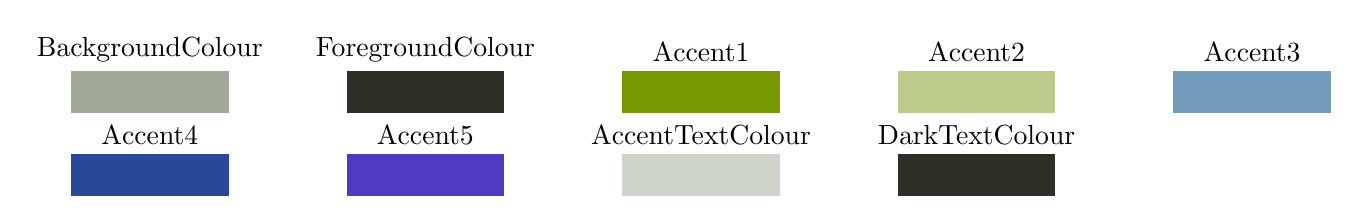
\begin{tikzpicture}
\definecolor{col}{HTML}{A0A998}
\fill[col] (0.0, -0.5em + 0em) rectangle (2.0, 1em + 0em) (1.0, 1em + 0em) node[above, text = black] {BackgroundColour};
\definecolor{col}{HTML}{2F2F27}
\fill[col] (3.5, -0.5em + 0em) rectangle (5.5, 1em + 0em) (4.5, 1em + 0em) node[above, text = black] {ForegroundColour};
\definecolor{col}{HTML}{779803}
\fill[col] (7.0, -0.5em + 0em) rectangle (9.0, 1em + 0em) (8.0, 1em + 0em) node[above, text = black] {Accent1};
\definecolor{col}{HTML}{BBCB8C}
\fill[col] (10.5, -0.5em + 0em) rectangle (12.5, 1em + 0em) (11.5, 1em + 0em) node[above, text = black] {Accent2};
\definecolor{col}{HTML}{749DBB}
\fill[col] (14.0, -0.5em + 0em) rectangle (16.0, 1em + 0em) (15.0, 1em + 0em) node[above, text = black] {Accent3};
\definecolor{col}{HTML}{28499A}
\fill[col] (0.0, -0.5em + -3em) rectangle (2.0, 1em + -3em) (1.0, 1em + -3em) node[above, text = black] {Accent4};
\definecolor{col}{HTML}{503AC1}
\fill[col] (3.5, -0.5em + -3em) rectangle (5.5, 1em + -3em) (4.5, 1em + -3em) node[above, text = black] {Accent5};
\definecolor{col}{HTML}{A0A998}
\fill[col!50!white] (7.0, -0.5em + -3em) rectangle (9.0, 1em + -3em) (8.0, 1em + -3em) node[above, text = black] {AccentTextColour};
\definecolor{col}{HTML}{2F2F27}
\fill[col] (10.5, -0.5em + -3em) rectangle (12.5, 1em + -3em) (11.5, 1em + -3em) node[above, text = black] {DarkTextColour};
\end{tikzpicture}

\subsection*{Module}
\subsubsection*{Light}
\noindent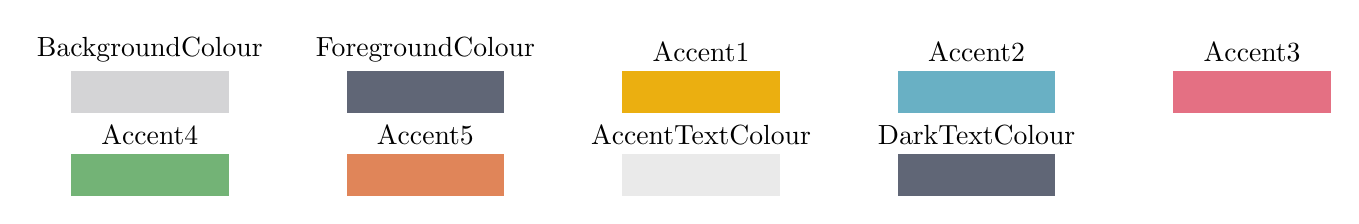
\begin{tikzpicture}
\definecolor{col}{HTML}{D4D4D6}
\fill[col] (0.0, -0.5em + 0em) rectangle (2.0, 1em + 0em) (1.0, 1em + 0em) node[above, text = black] {BackgroundColour};
\definecolor{col}{HTML}{606676}
\fill[col] (3.5, -0.5em + 0em) rectangle (5.5, 1em + 0em) (4.5, 1em + 0em) node[above, text = black] {ForegroundColour};
\definecolor{col}{HTML}{EBAF10}
\fill[col] (7.0, -0.5em + 0em) rectangle (9.0, 1em + 0em) (8.0, 1em + 0em) node[above, text = black] {Accent1};
\definecolor{col}{HTML}{69B0C4}
\fill[col] (10.5, -0.5em + 0em) rectangle (12.5, 1em + 0em) (11.5, 1em + 0em) node[above, text = black] {Accent2};
\definecolor{col}{HTML}{E47083}
\fill[col] (14.0, -0.5em + 0em) rectangle (16.0, 1em + 0em) (15.0, 1em + 0em) node[above, text = black] {Accent3};
\definecolor{col}{HTML}{73B376}
\fill[col] (0.0, -0.5em + -3em) rectangle (2.0, 1em + -3em) (1.0, 1em + -3em) node[above, text = black] {Accent4};
\definecolor{col}{HTML}{E08559}
\fill[col] (3.5, -0.5em + -3em) rectangle (5.5, 1em + -3em) (4.5, 1em + -3em) node[above, text = black] {Accent5};
\definecolor{col}{HTML}{D4D4D6}
\fill[col!50!white] (7.0, -0.5em + -3em) rectangle (9.0, 1em + -3em) (8.0, 1em + -3em) node[above, text = black] {AccentTextColour};
\definecolor{col}{HTML}{606676}
\fill[col] (10.5, -0.5em + -3em) rectangle (12.5, 1em + -3em) (11.5, 1em + -3em) node[above, text = black] {DarkTextColour};
\end{tikzpicture}

\subsection*{Newsprint}
\subsubsection*{Light}
\noindent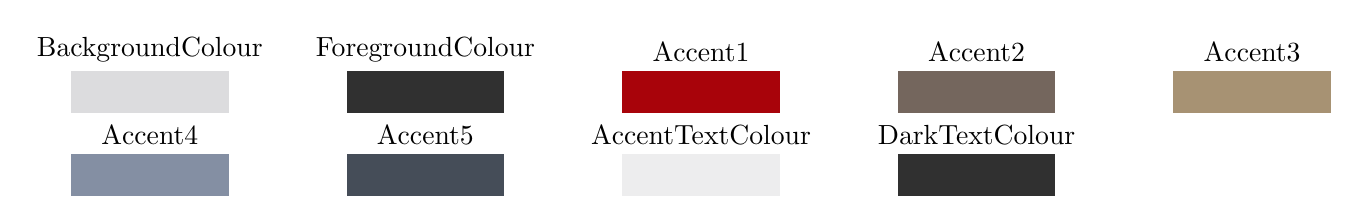
\begin{tikzpicture}
\definecolor{col}{HTML}{DCDCDE}
\fill[col] (0.0, -0.5em + 0em) rectangle (2.0, 1em + 0em) (1.0, 1em + 0em) node[above, text = black] {BackgroundColour};
\definecolor{col}{HTML}{303030}
\fill[col] (3.5, -0.5em + 0em) rectangle (5.5, 1em + 0em) (4.5, 1em + 0em) node[above, text = black] {ForegroundColour};
\definecolor{col}{HTML}{A8030A}
\fill[col] (7.0, -0.5em + 0em) rectangle (9.0, 1em + 0em) (8.0, 1em + 0em) node[above, text = black] {Accent1};
\definecolor{col}{HTML}{74665D}
\fill[col] (10.5, -0.5em + 0em) rectangle (12.5, 1em + 0em) (11.5, 1em + 0em) node[above, text = black] {Accent2};
\definecolor{col}{HTML}{A79273}
\fill[col] (14.0, -0.5em + 0em) rectangle (16.0, 1em + 0em) (15.0, 1em + 0em) node[above, text = black] {Accent3};
\definecolor{col}{HTML}{848FA3}
\fill[col] (0.0, -0.5em + -3em) rectangle (2.0, 1em + -3em) (1.0, 1em + -3em) node[above, text = black] {Accent4};
\definecolor{col}{HTML}{454D58}
\fill[col] (3.5, -0.5em + -3em) rectangle (5.5, 1em + -3em) (4.5, 1em + -3em) node[above, text = black] {Accent5};
\definecolor{col}{HTML}{DCDCDE}
\fill[col!50!white] (7.0, -0.5em + -3em) rectangle (9.0, 1em + -3em) (8.0, 1em + -3em) node[above, text = black] {AccentTextColour};
\definecolor{col}{HTML}{303030}
\fill[col] (10.5, -0.5em + -3em) rectangle (12.5, 1em + -3em) (11.5, 1em + -3em) node[above, text = black] {DarkTextColour};
\end{tikzpicture}

\subsection*{Orbit}
\subsubsection*{Light}
\noindent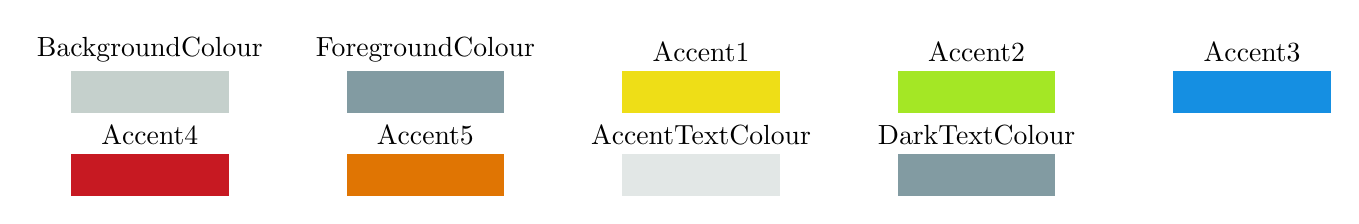
\begin{tikzpicture}
\definecolor{col}{HTML}{C5D0CC}
\fill[col] (0.0, -0.5em + 0em) rectangle (2.0, 1em + 0em) (1.0, 1em + 0em) node[above, text = black] {BackgroundColour};
\definecolor{col}{HTML}{829BA2}
\fill[col] (3.5, -0.5em + 0em) rectangle (5.5, 1em + 0em) (4.5, 1em + 0em) node[above, text = black] {ForegroundColour};
\definecolor{col}{HTML}{EEDE17}
\fill[col] (7.0, -0.5em + 0em) rectangle (9.0, 1em + 0em) (8.0, 1em + 0em) node[above, text = black] {Accent1};
\definecolor{col}{HTML}{A4E725}
\fill[col] (10.5, -0.5em + 0em) rectangle (12.5, 1em + 0em) (11.5, 1em + 0em) node[above, text = black] {Accent2};
\definecolor{col}{HTML}{158FE2}
\fill[col] (14.0, -0.5em + 0em) rectangle (16.0, 1em + 0em) (15.0, 1em + 0em) node[above, text = black] {Accent3};
\definecolor{col}{HTML}{C71922}
\fill[col] (0.0, -0.5em + -3em) rectangle (2.0, 1em + -3em) (1.0, 1em + -3em) node[above, text = black] {Accent4};
\definecolor{col}{HTML}{E07503}
\fill[col] (3.5, -0.5em + -3em) rectangle (5.5, 1em + -3em) (4.5, 1em + -3em) node[above, text = black] {Accent5};
\definecolor{col}{HTML}{C5D0CC}
\fill[col!50!white] (7.0, -0.5em + -3em) rectangle (9.0, 1em + -3em) (8.0, 1em + -3em) node[above, text = black] {AccentTextColour};
\definecolor{col}{HTML}{829BA2}
\fill[col] (10.5, -0.5em + -3em) rectangle (12.5, 1em + -3em) (11.5, 1em + -3em) node[above, text = black] {DarkTextColour};
\end{tikzpicture}

\subsection*{Perspective}
\subsubsection*{Light}
\noindent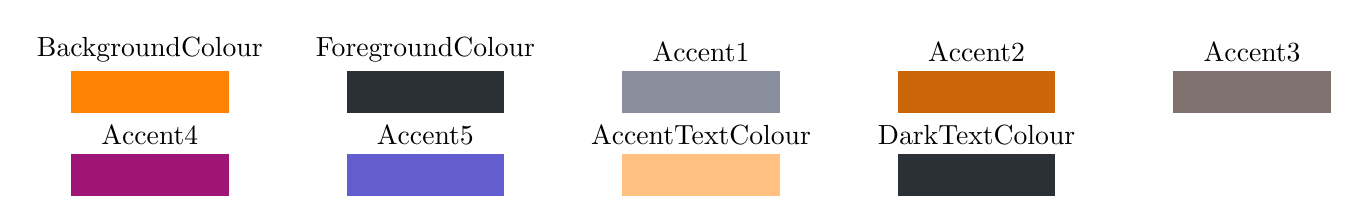
\begin{tikzpicture}
\definecolor{col}{HTML}{FF8202}
\fill[col] (0.0, -0.5em + 0em) rectangle (2.0, 1em + 0em) (1.0, 1em + 0em) node[above, text = black] {BackgroundColour};
\definecolor{col}{HTML}{2B3036}
\fill[col] (3.5, -0.5em + 0em) rectangle (5.5, 1em + 0em) (4.5, 1em + 0em) node[above, text = black] {ForegroundColour};
\definecolor{col}{HTML}{898F9D}
\fill[col] (7.0, -0.5em + 0em) rectangle (9.0, 1em + 0em) (8.0, 1em + 0em) node[above, text = black] {Accent1};
\definecolor{col}{HTML}{CA6509}
\fill[col] (10.5, -0.5em + 0em) rectangle (12.5, 1em + 0em) (11.5, 1em + 0em) node[above, text = black] {Accent2};
\definecolor{col}{HTML}{80726F}
\fill[col] (14.0, -0.5em + 0em) rectangle (16.0, 1em + 0em) (15.0, 1em + 0em) node[above, text = black] {Accent3};
\definecolor{col}{HTML}{9F1575}
\fill[col] (0.0, -0.5em + -3em) rectangle (2.0, 1em + -3em) (1.0, 1em + -3em) node[above, text = black] {Accent4};
\definecolor{col}{HTML}{625ECF}
\fill[col] (3.5, -0.5em + -3em) rectangle (5.5, 1em + -3em) (4.5, 1em + -3em) node[above, text = black] {Accent5};
\definecolor{col}{HTML}{FF8202}
\fill[col!50!white] (7.0, -0.5em + -3em) rectangle (9.0, 1em + -3em) (8.0, 1em + -3em) node[above, text = black] {AccentTextColour};
\definecolor{col}{HTML}{2B3036}
\fill[col] (10.5, -0.5em + -3em) rectangle (12.5, 1em + -3em) (11.5, 1em + -3em) node[above, text = black] {DarkTextColour};
\end{tikzpicture}

\subsection*{Perception}
\subsubsection*{Light}
\noindent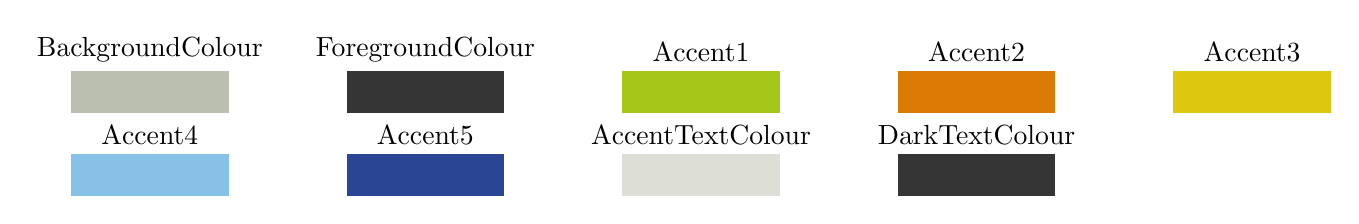
\begin{tikzpicture}
\definecolor{col}{HTML}{BBBFB0}
\fill[col] (0.0, -0.5em + 0em) rectangle (2.0, 1em + 0em) (1.0, 1em + 0em) node[above, text = black] {BackgroundColour};
\definecolor{col}{HTML}{353535}
\fill[col] (3.5, -0.5em + 0em) rectangle (5.5, 1em + 0em) (4.5, 1em + 0em) node[above, text = black] {ForegroundColour};
\definecolor{col}{HTML}{A5C719}
\fill[col] (7.0, -0.5em + 0em) rectangle (9.0, 1em + 0em) (8.0, 1em + 0em) node[above, text = black] {Accent1};
\definecolor{col}{HTML}{DA7B05}
\fill[col] (10.5, -0.5em + 0em) rectangle (12.5, 1em + 0em) (11.5, 1em + 0em) node[above, text = black] {Accent2};
\definecolor{col}{HTML}{DDC70F}
\fill[col] (14.0, -0.5em + 0em) rectangle (16.0, 1em + 0em) (15.0, 1em + 0em) node[above, text = black] {Accent3};
\definecolor{col}{HTML}{86C2E7}
\fill[col] (0.0, -0.5em + -3em) rectangle (2.0, 1em + -3em) (1.0, 1em + -3em) node[above, text = black] {Accent4};
\definecolor{col}{HTML}{2A4594}
\fill[col] (3.5, -0.5em + -3em) rectangle (5.5, 1em + -3em) (4.5, 1em + -3em) node[above, text = black] {Accent5};
\definecolor{col}{HTML}{BBBFB0}
\fill[col!50!white] (7.0, -0.5em + -3em) rectangle (9.0, 1em + -3em) (8.0, 1em + -3em) node[above, text = black] {AccentTextColour};
\definecolor{col}{HTML}{353535}
\fill[col] (10.5, -0.5em + -3em) rectangle (12.5, 1em + -3em) (11.5, 1em + -3em) node[above, text = black] {DarkTextColour};
\end{tikzpicture}

\subsection*{Paper}
\subsubsection*{Light}
\noindent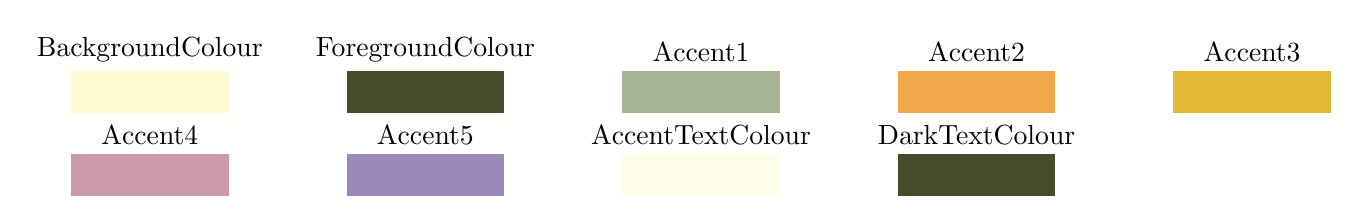
\begin{tikzpicture}
\definecolor{col}{HTML}{FDFBD4}
\fill[col] (0.0, -0.5em + 0em) rectangle (2.0, 1em + 0em) (1.0, 1em + 0em) node[above, text = black] {BackgroundColour};
\definecolor{col}{HTML}{454C2B}
\fill[col] (3.5, -0.5em + 0em) rectangle (5.5, 1em + 0em) (4.5, 1em + 0em) node[above, text = black] {ForegroundColour};
\definecolor{col}{HTML}{A6B397}
\fill[col] (7.0, -0.5em + 0em) rectangle (9.0, 1em + 0em) (8.0, 1em + 0em) node[above, text = black] {Accent1};
\definecolor{col}{HTML}{F1A84C}
\fill[col] (10.5, -0.5em + 0em) rectangle (12.5, 1em + 0em) (11.5, 1em + 0em) node[above, text = black] {Accent2};
\definecolor{col}{HTML}{E2BA36}
\fill[col] (14.0, -0.5em + 0em) rectangle (16.0, 1em + 0em) (15.0, 1em + 0em) node[above, text = black] {Accent3};
\definecolor{col}{HTML}{CC99AA}
\fill[col] (0.0, -0.5em + -3em) rectangle (2.0, 1em + -3em) (1.0, 1em + -3em) node[above, text = black] {Accent4};
\definecolor{col}{HTML}{9B89BB}
\fill[col] (3.5, -0.5em + -3em) rectangle (5.5, 1em + -3em) (4.5, 1em + -3em) node[above, text = black] {Accent5};
\definecolor{col}{HTML}{FDFBD4}
\fill[col!50!white] (7.0, -0.5em + -3em) rectangle (9.0, 1em + -3em) (8.0, 1em + -3em) node[above, text = black] {AccentTextColour};
\definecolor{col}{HTML}{454C2B}
\fill[col] (10.5, -0.5em + -3em) rectangle (12.5, 1em + -3em) (11.5, 1em + -3em) node[above, text = black] {DarkTextColour};
\end{tikzpicture}

\subsection*{Pixel}
\subsubsection*{Light}
\noindent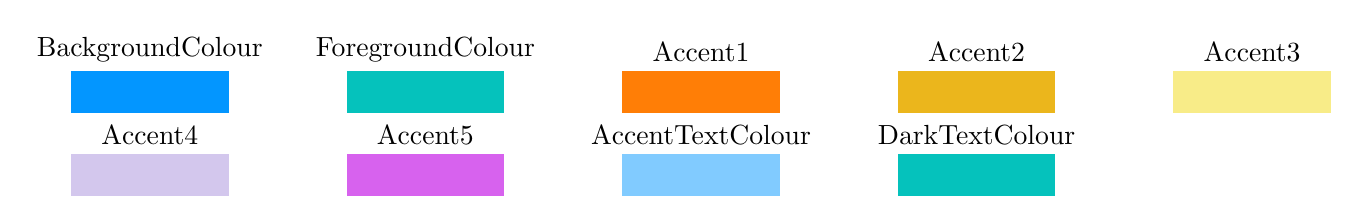
\begin{tikzpicture}
\definecolor{col}{HTML}{0396FF}
\fill[col] (0.0, -0.5em + 0em) rectangle (2.0, 1em + 0em) (1.0, 1em + 0em) node[above, text = black] {BackgroundColour};
\definecolor{col}{HTML}{05C2BC}
\fill[col] (3.5, -0.5em + 0em) rectangle (5.5, 1em + 0em) (4.5, 1em + 0em) node[above, text = black] {ForegroundColour};
\definecolor{col}{HTML}{FF7E06}
\fill[col] (7.0, -0.5em + 0em) rectangle (9.0, 1em + 0em) (8.0, 1em + 0em) node[above, text = black] {Accent1};
\definecolor{col}{HTML}{EBB61C}
\fill[col] (10.5, -0.5em + 0em) rectangle (12.5, 1em + 0em) (11.5, 1em + 0em) node[above, text = black] {Accent2};
\definecolor{col}{HTML}{F8EC88}
\fill[col] (14.0, -0.5em + 0em) rectangle (16.0, 1em + 0em) (15.0, 1em + 0em) node[above, text = black] {Accent3};
\definecolor{col}{HTML}{D3C7ED}
\fill[col] (0.0, -0.5em + -3em) rectangle (2.0, 1em + -3em) (1.0, 1em + -3em) node[above, text = black] {Accent4};
\definecolor{col}{HTML}{D762EE}
\fill[col] (3.5, -0.5em + -3em) rectangle (5.5, 1em + -3em) (4.5, 1em + -3em) node[above, text = black] {Accent5};
\definecolor{col}{HTML}{0396FF}
\fill[col!50!white] (7.0, -0.5em + -3em) rectangle (9.0, 1em + -3em) (8.0, 1em + -3em) node[above, text = black] {AccentTextColour};
\definecolor{col}{HTML}{05C2BC}
\fill[col] (10.5, -0.5em + -3em) rectangle (12.5, 1em + -3em) (11.5, 1em + -3em) node[above, text = black] {DarkTextColour};
\end{tikzpicture}

\subsection*{Plaza}
\subsubsection*{Light}
\noindent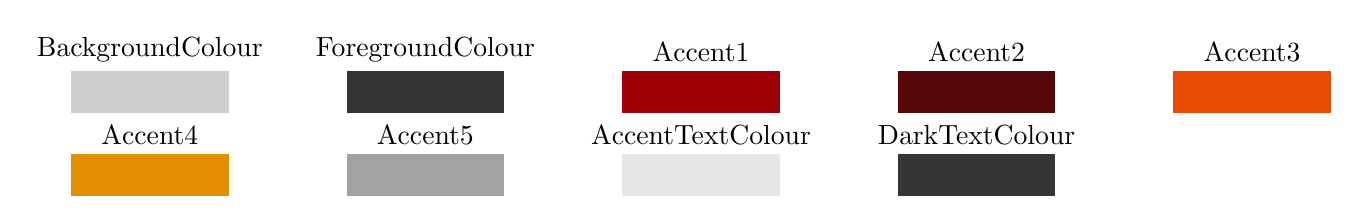
\begin{tikzpicture}
\definecolor{col}{HTML}{CECECE}
\fill[col] (0.0, -0.5em + 0em) rectangle (2.0, 1em + 0em) (1.0, 1em + 0em) node[above, text = black] {BackgroundColour};
\definecolor{col}{HTML}{353535}
\fill[col] (3.5, -0.5em + 0em) rectangle (5.5, 1em + 0em) (4.5, 1em + 0em) node[above, text = black] {ForegroundColour};
\definecolor{col}{HTML}{9C0006}
\fill[col] (7.0, -0.5em + 0em) rectangle (9.0, 1em + 0em) (8.0, 1em + 0em) node[above, text = black] {Accent1};
\definecolor{col}{HTML}{560808}
\fill[col] (10.5, -0.5em + 0em) rectangle (12.5, 1em + 0em) (11.5, 1em + 0em) node[above, text = black] {Accent2};
\definecolor{col}{HTML}{E84A01}
\fill[col] (14.0, -0.5em + 0em) rectangle (16.0, 1em + 0em) (15.0, 1em + 0em) node[above, text = black] {Accent3};
\definecolor{col}{HTML}{E58E03}
\fill[col] (0.0, -0.5em + -3em) rectangle (2.0, 1em + -3em) (1.0, 1em + -3em) node[above, text = black] {Accent4};
\definecolor{col}{HTML}{A3A3A3}
\fill[col] (3.5, -0.5em + -3em) rectangle (5.5, 1em + -3em) (4.5, 1em + -3em) node[above, text = black] {Accent5};
\definecolor{col}{HTML}{CECECE}
\fill[col!50!white] (7.0, -0.5em + -3em) rectangle (9.0, 1em + -3em) (8.0, 1em + -3em) node[above, text = black] {AccentTextColour};
\definecolor{col}{HTML}{353535}
\fill[col] (10.5, -0.5em + -3em) rectangle (12.5, 1em + -3em) (11.5, 1em + -3em) node[above, text = black] {DarkTextColour};
\end{tikzpicture}

\subsection*{Precedent}
\subsubsection*{Light}
\noindent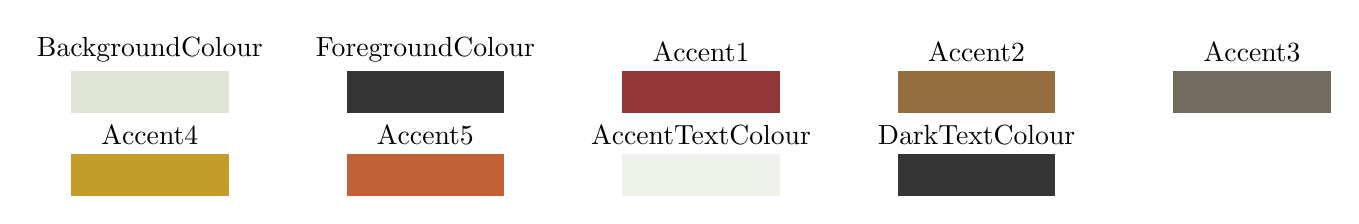
\begin{tikzpicture}
\definecolor{col}{HTML}{E0E4D5}
\fill[col] (0.0, -0.5em + 0em) rectangle (2.0, 1em + 0em) (1.0, 1em + 0em) node[above, text = black] {BackgroundColour};
\definecolor{col}{HTML}{353535}
\fill[col] (3.5, -0.5em + 0em) rectangle (5.5, 1em + 0em) (4.5, 1em + 0em) node[above, text = black] {ForegroundColour};
\definecolor{col}{HTML}{923637}
\fill[col] (7.0, -0.5em + 0em) rectangle (9.0, 1em + 0em) (8.0, 1em + 0em) node[above, text = black] {Accent1};
\definecolor{col}{HTML}{946E3F}
\fill[col] (10.5, -0.5em + 0em) rectangle (12.5, 1em + 0em) (11.5, 1em + 0em) node[above, text = black] {Accent2};
\definecolor{col}{HTML}{726C60}
\fill[col] (14.0, -0.5em + 0em) rectangle (16.0, 1em + 0em) (15.0, 1em + 0em) node[above, text = black] {Accent3};
\definecolor{col}{HTML}{C49C2B}
\fill[col] (0.0, -0.5em + -3em) rectangle (2.0, 1em + -3em) (1.0, 1em + -3em) node[above, text = black] {Accent4};
\definecolor{col}{HTML}{C16236}
\fill[col] (3.5, -0.5em + -3em) rectangle (5.5, 1em + -3em) (4.5, 1em + -3em) node[above, text = black] {Accent5};
\definecolor{col}{HTML}{E0E4D5}
\fill[col!50!white] (7.0, -0.5em + -3em) rectangle (9.0, 1em + -3em) (8.0, 1em + -3em) node[above, text = black] {AccentTextColour};
\definecolor{col}{HTML}{353535}
\fill[col] (10.5, -0.5em + -3em) rectangle (12.5, 1em + -3em) (11.5, 1em + -3em) node[above, text = black] {DarkTextColour};
\end{tikzpicture}

\subsection*{Saddle}
\subsubsection*{Light}
\noindent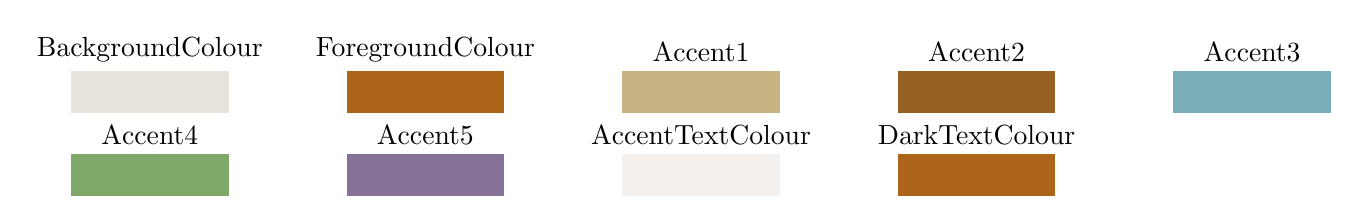
\begin{tikzpicture}
\definecolor{col}{HTML}{E7E2DC}
\fill[col] (0.0, -0.5em + 0em) rectangle (2.0, 1em + 0em) (1.0, 1em + 0em) node[above, text = black] {BackgroundColour};
\definecolor{col}{HTML}{AC641A}
\fill[col] (3.5, -0.5em + 0em) rectangle (5.5, 1em + 0em) (4.5, 1em + 0em) node[above, text = black] {ForegroundColour};
\definecolor{col}{HTML}{C6B482}
\fill[col] (7.0, -0.5em + 0em) rectangle (9.0, 1em + 0em) (8.0, 1em + 0em) node[above, text = black] {Accent1};
\definecolor{col}{HTML}{966020}
\fill[col] (10.5, -0.5em + 0em) rectangle (12.5, 1em + 0em) (11.5, 1em + 0em) node[above, text = black] {Accent2};
\definecolor{col}{HTML}{79ADB8}
\fill[col] (14.0, -0.5em + 0em) rectangle (16.0, 1em + 0em) (15.0, 1em + 0em) node[above, text = black] {Accent3};
\definecolor{col}{HTML}{80A869}
\fill[col] (0.0, -0.5em + -3em) rectangle (2.0, 1em + -3em) (1.0, 1em + -3em) node[above, text = black] {Accent4};
\definecolor{col}{HTML}{867297}
\fill[col] (3.5, -0.5em + -3em) rectangle (5.5, 1em + -3em) (4.5, 1em + -3em) node[above, text = black] {Accent5};
\definecolor{col}{HTML}{E7E2DC}
\fill[col!50!white] (7.0, -0.5em + -3em) rectangle (9.0, 1em + -3em) (8.0, 1em + -3em) node[above, text = black] {AccentTextColour};
\definecolor{col}{HTML}{AC641A}
\fill[col] (10.5, -0.5em + -3em) rectangle (12.5, 1em + -3em) (11.5, 1em + -3em) node[above, text = black] {DarkTextColour};
\end{tikzpicture}

\subsection*{Revolution}
\subsubsection*{Light}
\noindent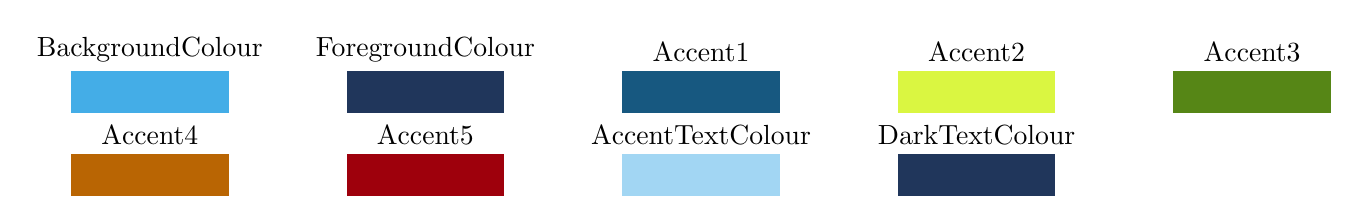
\begin{tikzpicture}
\definecolor{col}{HTML}{44ADE7}
\fill[col] (0.0, -0.5em + 0em) rectangle (2.0, 1em + 0em) (1.0, 1em + 0em) node[above, text = black] {BackgroundColour};
\definecolor{col}{HTML}{20365B}
\fill[col] (3.5, -0.5em + 0em) rectangle (5.5, 1em + 0em) (4.5, 1em + 0em) node[above, text = black] {ForegroundColour};
\definecolor{col}{HTML}{175880}
\fill[col] (7.0, -0.5em + 0em) rectangle (9.0, 1em + 0em) (8.0, 1em + 0em) node[above, text = black] {Accent1};
\definecolor{col}{HTML}{DAF641}
\fill[col] (10.5, -0.5em + 0em) rectangle (12.5, 1em + 0em) (11.5, 1em + 0em) node[above, text = black] {Accent2};
\definecolor{col}{HTML}{568616}
\fill[col] (14.0, -0.5em + 0em) rectangle (16.0, 1em + 0em) (15.0, 1em + 0em) node[above, text = black] {Accent3};
\definecolor{col}{HTML}{B96503}
\fill[col] (0.0, -0.5em + -3em) rectangle (2.0, 1em + -3em) (1.0, 1em + -3em) node[above, text = black] {Accent4};
\definecolor{col}{HTML}{9E000C}
\fill[col] (3.5, -0.5em + -3em) rectangle (5.5, 1em + -3em) (4.5, 1em + -3em) node[above, text = black] {Accent5};
\definecolor{col}{HTML}{44ADE7}
\fill[col!50!white] (7.0, -0.5em + -3em) rectangle (9.0, 1em + -3em) (8.0, 1em + -3em) node[above, text = black] {AccentTextColour};
\definecolor{col}{HTML}{20365B}
\fill[col] (10.5, -0.5em + -3em) rectangle (12.5, 1em + -3em) (11.5, 1em + -3em) node[above, text = black] {DarkTextColour};
\end{tikzpicture}

\subsection*{Pushpin}
\subsubsection*{Light}
\noindent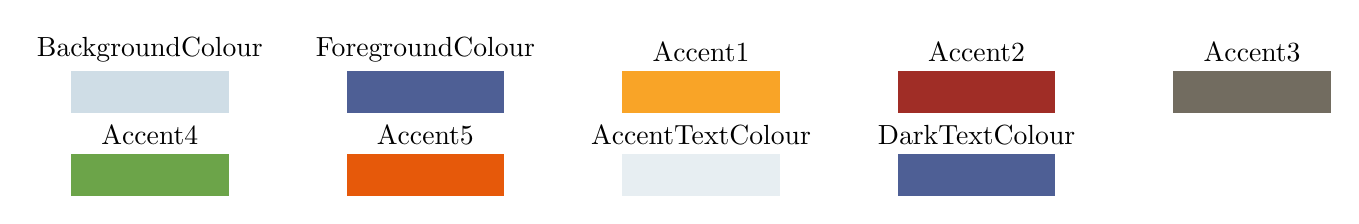
\begin{tikzpicture}
\definecolor{col}{HTML}{CFDDE6}
\fill[col] (0.0, -0.5em + 0em) rectangle (2.0, 1em + 0em) (1.0, 1em + 0em) node[above, text = black] {BackgroundColour};
\definecolor{col}{HTML}{4E5F95}
\fill[col] (3.5, -0.5em + 0em) rectangle (5.5, 1em + 0em) (4.5, 1em + 0em) node[above, text = black] {ForegroundColour};
\definecolor{col}{HTML}{F9A427}
\fill[col] (7.0, -0.5em + 0em) rectangle (9.0, 1em + 0em) (8.0, 1em + 0em) node[above, text = black] {Accent1};
\definecolor{col}{HTML}{A02D26}
\fill[col] (10.5, -0.5em + 0em) rectangle (12.5, 1em + 0em) (11.5, 1em + 0em) node[above, text = black] {Accent2};
\definecolor{col}{HTML}{726C60}
\fill[col] (14.0, -0.5em + 0em) rectangle (16.0, 1em + 0em) (15.0, 1em + 0em) node[above, text = black] {Accent3};
\definecolor{col}{HTML}{6CA449}
\fill[col] (0.0, -0.5em + -3em) rectangle (2.0, 1em + -3em) (1.0, 1em + -3em) node[above, text = black] {Accent4};
\definecolor{col}{HTML}{E6590A}
\fill[col] (3.5, -0.5em + -3em) rectangle (5.5, 1em + -3em) (4.5, 1em + -3em) node[above, text = black] {Accent5};
\definecolor{col}{HTML}{CFDDE6}
\fill[col!50!white] (7.0, -0.5em + -3em) rectangle (9.0, 1em + -3em) (8.0, 1em + -3em) node[above, text = black] {AccentTextColour};
\definecolor{col}{HTML}{4E5F95}
\fill[col] (10.5, -0.5em + -3em) rectangle (12.5, 1em + -3em) (11.5, 1em + -3em) node[above, text = black] {DarkTextColour};
\end{tikzpicture}

\subsection*{Sketchbook}
\subsubsection*{Light}
\noindent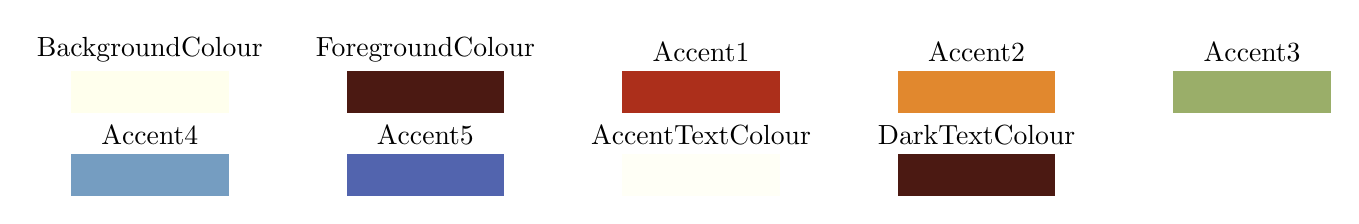
\begin{tikzpicture}
\definecolor{col}{HTML}{FFFFED}
\fill[col] (0.0, -0.5em + 0em) rectangle (2.0, 1em + 0em) (1.0, 1em + 0em) node[above, text = black] {BackgroundColour};
\definecolor{col}{HTML}{4B1912}
\fill[col] (3.5, -0.5em + 0em) rectangle (5.5, 1em + 0em) (4.5, 1em + 0em) node[above, text = black] {ForegroundColour};
\definecolor{col}{HTML}{AC2F1B}
\fill[col] (7.0, -0.5em + 0em) rectangle (9.0, 1em + 0em) (8.0, 1em + 0em) node[above, text = black] {Accent1};
\definecolor{col}{HTML}{E1882E}
\fill[col] (10.5, -0.5em + 0em) rectangle (12.5, 1em + 0em) (11.5, 1em + 0em) node[above, text = black] {Accent2};
\definecolor{col}{HTML}{9AAE69}
\fill[col] (14.0, -0.5em + 0em) rectangle (16.0, 1em + 0em) (15.0, 1em + 0em) node[above, text = black] {Accent3};
\definecolor{col}{HTML}{759DC1}
\fill[col] (0.0, -0.5em + -3em) rectangle (2.0, 1em + -3em) (1.0, 1em + -3em) node[above, text = black] {Accent4};
\definecolor{col}{HTML}{5264AE}
\fill[col] (3.5, -0.5em + -3em) rectangle (5.5, 1em + -3em) (4.5, 1em + -3em) node[above, text = black] {Accent5};
\definecolor{col}{HTML}{FFFFED}
\fill[col!50!white] (7.0, -0.5em + -3em) rectangle (9.0, 1em + -3em) (8.0, 1em + -3em) node[above, text = black] {AccentTextColour};
\definecolor{col}{HTML}{4B1912}
\fill[col] (10.5, -0.5em + -3em) rectangle (12.5, 1em + -3em) (11.5, 1em + -3em) node[above, text = black] {DarkTextColour};
\end{tikzpicture}

\subsection*{Sky}
\subsubsection*{Light}
\noindent\begin{tikzpicture}
\definecolor{col}{HTML}{67BBDF}
\fill[col] (0.0, -0.5em + 0em) rectangle (2.0, 1em + 0em) (1.0, 1em + 0em) node[above, text = black] {BackgroundColour};
\definecolor{col}{HTML}{1B87B6}
\fill[col] (3.5, -0.5em + 0em) rectangle (5.5, 1em + 0em) (4.5, 1em + 0em) node[above, text = black] {ForegroundColour};
\definecolor{col}{HTML}{10346E}
\fill[col] (7.0, -0.5em + 0em) rectangle (9.0, 1em + 0em) (8.0, 1em + 0em) node[above, text = black] {Accent1};
\definecolor{col}{HTML}{97D7F3}
\fill[col] (10.5, -0.5em + 0em) rectangle (12.5, 1em + 0em) (11.5, 1em + 0em) node[above, text = black] {Accent2};
\definecolor{col}{HTML}{F6CE0C}
\fill[col] (14.0, -0.5em + 0em) rectangle (16.0, 1em + 0em) (15.0, 1em + 0em) node[above, text = black] {Accent3};
\definecolor{col}{HTML}{EF6914}
\fill[col] (0.0, -0.5em + -3em) rectangle (2.0, 1em + -3em) (1.0, 1em + -3em) node[above, text = black] {Accent4};
\definecolor{col}{HTML}{BE6708}
\fill[col] (3.5, -0.5em + -3em) rectangle (5.5, 1em + -3em) (4.5, 1em + -3em) node[above, text = black] {Accent5};
\definecolor{col}{HTML}{67BBDF}
\fill[col!50!white] (7.0, -0.5em + -3em) rectangle (9.0, 1em + -3em) (8.0, 1em + -3em) node[above, text = black] {AccentTextColour};
\definecolor{col}{HTML}{1B87B6}
\fill[col] (10.5, -0.5em + -3em) rectangle (12.5, 1em + -3em) (11.5, 1em + -3em) node[above, text = black] {DarkTextColour};
\end{tikzpicture}

\subsection*{Slipstream}
\subsubsection*{Light}
\noindent\begin{tikzpicture}
\definecolor{col}{HTML}{BDDDF4}
\fill[col] (0.0, -0.5em + 0em) rectangle (2.0, 1em + 0em) (1.0, 1em + 0em) node[above, text = black] {BackgroundColour};
\definecolor{col}{HTML}{1F243A}
\fill[col] (3.5, -0.5em + 0em) rectangle (5.5, 1em + 0em) (4.5, 1em + 0em) node[above, text = black] {ForegroundColour};
\definecolor{col}{HTML}{5468BF}
\fill[col] (7.0, -0.5em + 0em) rectangle (9.0, 1em + 0em) (8.0, 1em + 0em) node[above, text = black] {Accent1};
\definecolor{col}{HTML}{61CCEC}
\fill[col] (10.5, -0.5em + 0em) rectangle (12.5, 1em + 0em) (11.5, 1em + 0em) node[above, text = black] {Accent2};
\definecolor{col}{HTML}{AEE65D}
\fill[col] (14.0, -0.5em + 0em) rectangle (16.0, 1em + 0em) (15.0, 1em + 0em) node[above, text = black] {Accent3};
\definecolor{col}{HTML}{63CEB0}
\fill[col] (0.0, -0.5em + -3em) rectangle (2.0, 1em + -3em) (1.0, 1em + -3em) node[above, text = black] {Accent4};
\definecolor{col}{HTML}{F48432}
\fill[col] (3.5, -0.5em + -3em) rectangle (5.5, 1em + -3em) (4.5, 1em + -3em) node[above, text = black] {Accent5};
\definecolor{col}{HTML}{BDDDF4}
\fill[col!50!white] (7.0, -0.5em + -3em) rectangle (9.0, 1em + -3em) (8.0, 1em + -3em) node[above, text = black] {AccentTextColour};
\definecolor{col}{HTML}{1F243A}
\fill[col] (10.5, -0.5em + -3em) rectangle (12.5, 1em + -3em) (11.5, 1em + -3em) node[above, text = black] {DarkTextColour};
\end{tikzpicture}

\subsection*{Spectrum}
\subsubsection*{Light}
\noindent\begin{tikzpicture}
\definecolor{col}{HTML}{E9E8E6}
\fill[col] (0.0, -0.5em + 0em) rectangle (2.0, 1em + 0em) (1.0, 1em + 0em) node[above, text = black] {BackgroundColour};
\definecolor{col}{HTML}{282830}
\fill[col] (3.5, -0.5em + 0em) rectangle (5.5, 1em + 0em) (4.5, 1em + 0em) node[above, text = black] {ForegroundColour};
\definecolor{col}{HTML}{9C0006}
\fill[col] (7.0, -0.5em + 0em) rectangle (9.0, 1em + 0em) (8.0, 1em + 0em) node[above, text = black] {Accent1};
\definecolor{col}{HTML}{FE6905}
\fill[col] (10.5, -0.5em + 0em) rectangle (12.5, 1em + 0em) (11.5, 1em + 0em) node[above, text = black] {Accent2};
\definecolor{col}{HTML}{F8BF0D}
\fill[col] (14.0, -0.5em + 0em) rectangle (16.0, 1em + 0em) (15.0, 1em + 0em) node[above, text = black] {Accent3};
\definecolor{col}{HTML}{9DCB09}
\fill[col] (0.0, -0.5em + -3em) rectangle (2.0, 1em + -3em) (1.0, 1em + -3em) node[above, text = black] {Accent4};
\definecolor{col}{HTML}{598A00}
\fill[col] (3.5, -0.5em + -3em) rectangle (5.5, 1em + -3em) (4.5, 1em + -3em) node[above, text = black] {Accent5};
\definecolor{col}{HTML}{E9E8E6}
\fill[col!50!white] (7.0, -0.5em + -3em) rectangle (9.0, 1em + -3em) (8.0, 1em + -3em) node[above, text = black] {AccentTextColour};
\definecolor{col}{HTML}{282830}
\fill[col] (10.5, -0.5em + -3em) rectangle (12.5, 1em + -3em) (11.5, 1em + -3em) node[above, text = black] {DarkTextColour};
\end{tikzpicture}

\subsection*{Solstice}
\subsubsection*{Light}
\noindent\begin{tikzpicture}
\definecolor{col}{HTML}{E2DDCA}
\fill[col] (0.0, -0.5em + 0em) rectangle (2.0, 1em + 0em) (1.0, 1em + 0em) node[above, text = black] {BackgroundColour};
\definecolor{col}{HTML}{492B23}
\fill[col] (3.5, -0.5em + 0em) rectangle (5.5, 1em + 0em) (4.5, 1em + 0em) node[above, text = black] {ForegroundColour};
\definecolor{col}{HTML}{428FA3}
\fill[col] (7.0, -0.5em + 0em) rectangle (9.0, 1em + 0em) (8.0, 1em + 0em) node[above, text = black] {Accent1};
\definecolor{col}{HTML}{FCBB15}
\fill[col] (10.5, -0.5em + 0em) rectangle (12.5, 1em + 0em) (11.5, 1em + 0em) node[above, text = black] {Accent2};
\definecolor{col}{HTML}{C42E37}
\fill[col] (14.0, -0.5em + 0em) rectangle (16.0, 1em + 0em) (15.0, 1em + 0em) node[above, text = black] {Accent3};
\definecolor{col}{HTML}{8AAB38}
\fill[col] (0.0, -0.5em + -3em) rectangle (2.0, 1em + -3em) (1.0, 1em + -3em) node[above, text = black] {Accent4};
\definecolor{col}{HTML}{93460E}
\fill[col] (3.5, -0.5em + -3em) rectangle (5.5, 1em + -3em) (4.5, 1em + -3em) node[above, text = black] {Accent5};
\definecolor{col}{HTML}{E2DDCA}
\fill[col!50!white] (7.0, -0.5em + -3em) rectangle (9.0, 1em + -3em) (8.0, 1em + -3em) node[above, text = black] {AccentTextColour};
\definecolor{col}{HTML}{492B23}
\fill[col] (10.5, -0.5em + -3em) rectangle (12.5, 1em + -3em) (11.5, 1em + -3em) node[above, text = black] {DarkTextColour};
\end{tikzpicture}

\subsection*{SoHo}
\subsubsection*{Light}
\noindent\begin{tikzpicture}
\definecolor{col}{HTML}{CDD8DC}
\fill[col] (0.0, -0.5em + 0em) rectangle (2.0, 1em + 0em) (1.0, 1em + 0em) node[above, text = black] {BackgroundColour};
\definecolor{col}{HTML}{442723}
\fill[col] (3.5, -0.5em + 0em) rectangle (5.5, 1em + 0em) (4.5, 1em + 0em) node[above, text = black] {ForegroundColour};
\definecolor{col}{HTML}{656661}
\fill[col] (7.0, -0.5em + 0em) rectangle (9.0, 1em + 0em) (8.0, 1em + 0em) node[above, text = black] {Accent1};
\definecolor{col}{HTML}{8F5138}
\fill[col] (10.5, -0.5em + 0em) rectangle (12.5, 1em + 0em) (11.5, 1em + 0em) node[above, text = black] {Accent2};
\definecolor{col}{HTML}{635643}
\fill[col] (14.0, -0.5em + 0em) rectangle (16.0, 1em + 0em) (15.0, 1em + 0em) node[above, text = black] {Accent3};
\definecolor{col}{HTML}{848160}
\fill[col] (0.0, -0.5em + -3em) rectangle (2.0, 1em + -3em) (1.0, 1em + -3em) node[above, text = black] {Accent4};
\definecolor{col}{HTML}{ADA252}
\fill[col] (3.5, -0.5em + -3em) rectangle (5.5, 1em + -3em) (4.5, 1em + -3em) node[above, text = black] {Accent5};
\definecolor{col}{HTML}{CDD8DC}
\fill[col!50!white] (7.0, -0.5em + -3em) rectangle (9.0, 1em + -3em) (8.0, 1em + -3em) node[above, text = black] {AccentTextColour};
\definecolor{col}{HTML}{442723}
\fill[col] (10.5, -0.5em + -3em) rectangle (12.5, 1em + -3em) (11.5, 1em + -3em) node[above, text = black] {DarkTextColour};
\end{tikzpicture}

\subsection*{Story}
\subsubsection*{Light}
\noindent\begin{tikzpicture}
\definecolor{col}{HTML}{CCD4D7}
\fill[col] (0.0, -0.5em + 0em) rectangle (2.0, 1em + 0em) (1.0, 1em + 0em) node[above, text = black] {BackgroundColour};
\definecolor{col}{HTML}{242424}
\fill[col] (3.5, -0.5em + 0em) rectangle (5.5, 1em + 0em) (4.5, 1em + 0em) node[above, text = black] {ForegroundColour};
\definecolor{col}{HTML}{1985C3}
\fill[col] (7.0, -0.5em + 0em) rectangle (9.0, 1em + 0em) (8.0, 1em + 0em) node[above, text = black] {Accent1};
\definecolor{col}{HTML}{6D328E}
\fill[col] (10.5, -0.5em + 0em) rectangle (12.5, 1em + 0em) (11.5, 1em + 0em) node[above, text = black] {Accent2};
\definecolor{col}{HTML}{B70E25}
\fill[col] (14.0, -0.5em + 0em) rectangle (16.0, 1em + 0em) (15.0, 1em + 0em) node[above, text = black] {Accent3};
\definecolor{col}{HTML}{E1950C}
\fill[col] (0.0, -0.5em + -3em) rectangle (2.0, 1em + -3em) (1.0, 1em + -3em) node[above, text = black] {Accent4};
\definecolor{col}{HTML}{5D9436}
\fill[col] (3.5, -0.5em + -3em) rectangle (5.5, 1em + -3em) (4.5, 1em + -3em) node[above, text = black] {Accent5};
\definecolor{col}{HTML}{CCD4D7}
\fill[col!50!white] (7.0, -0.5em + -3em) rectangle (9.0, 1em + -3em) (8.0, 1em + -3em) node[above, text = black] {AccentTextColour};
\definecolor{col}{HTML}{242424}
\fill[col] (10.5, -0.5em + -3em) rectangle (12.5, 1em + -3em) (11.5, 1em + -3em) node[above, text = black] {DarkTextColour};
\end{tikzpicture}

\subsection*{Summer}
\subsubsection*{Light}
\noindent\begin{tikzpicture}
\definecolor{col}{HTML}{E9BB1F}
\fill[col] (0.0, -0.5em + 0em) rectangle (2.0, 1em + 0em) (1.0, 1em + 0em) node[above, text = black] {BackgroundColour};
\definecolor{col}{HTML}{C8660B}
\fill[col] (3.5, -0.5em + 0em) rectangle (5.5, 1em + 0em) (4.5, 1em + 0em) node[above, text = black] {ForegroundColour};
\definecolor{col}{HTML}{5DA8BF}
\fill[col] (7.0, -0.5em + 0em) rectangle (9.0, 1em + 0em) (8.0, 1em + 0em) node[above, text = black] {Accent1};
\definecolor{col}{HTML}{59BDA5}
\fill[col] (10.5, -0.5em + 0em) rectangle (12.5, 1em + 0em) (11.5, 1em + 0em) node[above, text = black] {Accent2};
\definecolor{col}{HTML}{81BD5D}
\fill[col] (14.0, -0.5em + 0em) rectangle (16.0, 1em + 0em) (15.0, 1em + 0em) node[above, text = black] {Accent3};
\definecolor{col}{HTML}{E1E054}
\fill[col] (0.0, -0.5em + -3em) rectangle (2.0, 1em + -3em) (1.0, 1em + -3em) node[above, text = black] {Accent4};
\definecolor{col}{HTML}{B44C27}
\fill[col] (3.5, -0.5em + -3em) rectangle (5.5, 1em + -3em) (4.5, 1em + -3em) node[above, text = black] {Accent5};
\definecolor{col}{HTML}{E9BB1F}
\fill[col!50!white] (7.0, -0.5em + -3em) rectangle (9.0, 1em + -3em) (8.0, 1em + -3em) node[above, text = black] {AccentTextColour};
\definecolor{col}{HTML}{C8660B}
\fill[col] (10.5, -0.5em + -3em) rectangle (12.5, 1em + -3em) (11.5, 1em + -3em) node[above, text = black] {DarkTextColour};
\end{tikzpicture}

\subsection*{Technic}
\subsubsection*{Light}
\noindent\begin{tikzpicture}
\definecolor{col}{HTML}{D3D2D0}
\fill[col] (0.0, -0.5em + 0em) rectangle (2.0, 1em + 0em) (1.0, 1em + 0em) node[above, text = black] {BackgroundColour};
\definecolor{col}{HTML}{3D3D3D}
\fill[col] (3.5, -0.5em + 0em) rectangle (5.5, 1em + 0em) (4.5, 1em + 0em) node[above, text = black] {ForegroundColour};
\definecolor{col}{HTML}{729EA9}
\fill[col] (7.0, -0.5em + 0em) rectangle (9.0, 1em + 0em) (8.0, 1em + 0em) node[above, text = black] {Accent1};
\definecolor{col}{HTML}{C4B011}
\fill[col] (10.5, -0.5em + 0em) rectangle (12.5, 1em + 0em) (11.5, 1em + 0em) node[above, text = black] {Accent2};
\definecolor{col}{HTML}{8F8BA2}
\fill[col] (14.0, -0.5em + 0em) rectangle (16.0, 1em + 0em) (15.0, 1em + 0em) node[above, text = black] {Accent3};
\definecolor{col}{HTML}{768463}
\fill[col] (0.0, -0.5em + -3em) rectangle (2.0, 1em + -3em) (1.0, 1em + -3em) node[above, text = black] {Accent4};
\definecolor{col}{HTML}{9F957A}
\fill[col] (3.5, -0.5em + -3em) rectangle (5.5, 1em + -3em) (4.5, 1em + -3em) node[above, text = black] {Accent5};
\definecolor{col}{HTML}{D3D2D0}
\fill[col!50!white] (7.0, -0.5em + -3em) rectangle (9.0, 1em + -3em) (8.0, 1em + -3em) node[above, text = black] {AccentTextColour};
\definecolor{col}{HTML}{3D3D3D}
\fill[col] (10.5, -0.5em + -3em) rectangle (12.5, 1em + -3em) (11.5, 1em + -3em) node[above, text = black] {DarkTextColour};
\end{tikzpicture}

\subsection*{Twilight}
\subsubsection*{Light}
\noindent\begin{tikzpicture}
\definecolor{col}{HTML}{E7E8ED}
\fill[col] (0.0, -0.5em + 0em) rectangle (2.0, 1em + 0em) (1.0, 1em + 0em) node[above, text = black] {BackgroundColour};
\definecolor{col}{HTML}{25233B}
\fill[col] (3.5, -0.5em + 0em) rectangle (5.5, 1em + 0em) (4.5, 1em + 0em) node[above, text = black] {ForegroundColour};
\definecolor{col}{HTML}{E2BF49}
\fill[col] (7.0, -0.5em + 0em) rectangle (9.0, 1em + 0em) (8.0, 1em + 0em) node[above, text = black] {Accent1};
\definecolor{col}{HTML}{8EC1C5}
\fill[col] (10.5, -0.5em + 0em) rectangle (12.5, 1em + 0em) (11.5, 1em + 0em) node[above, text = black] {Accent2};
\definecolor{col}{HTML}{E09031}
\fill[col] (14.0, -0.5em + 0em) rectangle (16.0, 1em + 0em) (15.0, 1em + 0em) node[above, text = black] {Accent3};
\definecolor{col}{HTML}{919BD8}
\fill[col] (0.0, -0.5em + -3em) rectangle (2.0, 1em + -3em) (1.0, 1em + -3em) node[above, text = black] {Accent4};
\definecolor{col}{HTML}{869B4E}
\fill[col] (3.5, -0.5em + -3em) rectangle (5.5, 1em + -3em) (4.5, 1em + -3em) node[above, text = black] {Accent5};
\definecolor{col}{HTML}{E7E8ED}
\fill[col!50!white] (7.0, -0.5em + -3em) rectangle (9.0, 1em + -3em) (8.0, 1em + -3em) node[above, text = black] {AccentTextColour};
\definecolor{col}{HTML}{25233B}
\fill[col] (10.5, -0.5em + -3em) rectangle (12.5, 1em + -3em) (11.5, 1em + -3em) node[above, text = black] {DarkTextColour};
\end{tikzpicture}

\subsection*{Travelouge}
\subsubsection*{Light}
\noindent\begin{tikzpicture}
\definecolor{col}{HTML}{816B39}
\fill[col] (0.0, -0.5em + 0em) rectangle (2.0, 1em + 0em) (1.0, 1em + 0em) node[above, text = black] {BackgroundColour};
\definecolor{col}{HTML}{2E271F}
\fill[col] (3.5, -0.5em + 0em) rectangle (5.5, 1em + 0em) (4.5, 1em + 0em) node[above, text = black] {ForegroundColour};
\definecolor{col}{HTML}{BC4B21}
\fill[col] (7.0, -0.5em + 0em) rectangle (9.0, 1em + 0em) (8.0, 1em + 0em) node[above, text = black] {Accent1};
\definecolor{col}{HTML}{A3262C}
\fill[col] (10.5, -0.5em + 0em) rectangle (12.5, 1em + 0em) (11.5, 1em + 0em) node[above, text = black] {Accent2};
\definecolor{col}{HTML}{49759A}
\fill[col] (14.0, -0.5em + 0em) rectangle (16.0, 1em + 0em) (15.0, 1em + 0em) node[above, text = black] {Accent3};
\definecolor{col}{HTML}{665F95}
\fill[col] (0.0, -0.5em + -3em) rectangle (2.0, 1em + -3em) (1.0, 1em + -3em) node[above, text = black] {Accent4};
\definecolor{col}{HTML}{689155}
\fill[col] (3.5, -0.5em + -3em) rectangle (5.5, 1em + -3em) (4.5, 1em + -3em) node[above, text = black] {Accent5};
\definecolor{col}{HTML}{816B39}
\fill[col!50!white] (7.0, -0.5em + -3em) rectangle (9.0, 1em + -3em) (8.0, 1em + -3em) node[above, text = black] {AccentTextColour};
\definecolor{col}{HTML}{2E271F}
\fill[col] (10.5, -0.5em + -3em) rectangle (12.5, 1em + -3em) (11.5, 1em + -3em) node[above, text = black] {DarkTextColour};
\end{tikzpicture}

\subsection*{Tradition}
\subsubsection*{Light}
\noindent\begin{tikzpicture}
\definecolor{col}{HTML}{CB9113}
\fill[col] (0.0, -0.5em + 0em) rectangle (2.0, 1em + 0em) (1.0, 1em + 0em) node[above, text = black] {BackgroundColour};
\definecolor{col}{HTML}{5A491B}
\fill[col] (3.5, -0.5em + 0em) rectangle (5.5, 1em + 0em) (4.5, 1em + 0em) node[above, text = black] {ForegroundColour};
\definecolor{col}{HTML}{694B17}
\fill[col] (7.0, -0.5em + 0em) rectangle (9.0, 1em + 0em) (8.0, 1em + 0em) node[above, text = black] {Accent1};
\definecolor{col}{HTML}{73121B}
\fill[col] (10.5, -0.5em + 0em) rectangle (12.5, 1em + 0em) (11.5, 1em + 0em) node[above, text = black] {Accent2};
\definecolor{col}{HTML}{8F824B}
\fill[col] (14.0, -0.5em + 0em) rectangle (16.0, 1em + 0em) (15.0, 1em + 0em) node[above, text = black] {Accent3};
\definecolor{col}{HTML}{46425B}
\fill[col] (0.0, -0.5em + -3em) rectangle (2.0, 1em + -3em) (1.0, 1em + -3em) node[above, text = black] {Accent4};
\definecolor{col}{HTML}{601742}
\fill[col] (3.5, -0.5em + -3em) rectangle (5.5, 1em + -3em) (4.5, 1em + -3em) node[above, text = black] {Accent5};
\definecolor{col}{HTML}{CB9113}
\fill[col!50!white] (7.0, -0.5em + -3em) rectangle (9.0, 1em + -3em) (8.0, 1em + -3em) node[above, text = black] {AccentTextColour};
\definecolor{col}{HTML}{5A491B}
\fill[col] (10.5, -0.5em + -3em) rectangle (12.5, 1em + -3em) (11.5, 1em + -3em) node[above, text = black] {DarkTextColour};
\end{tikzpicture}

\subsection*{Urban Pop}
\subsubsection*{Light}
\noindent\begin{tikzpicture}
\definecolor{col}{HTML}{D4D4D4}
\fill[col] (0.0, -0.5em + 0em) rectangle (2.0, 1em + 0em) (1.0, 1em + 0em) node[above, text = black] {BackgroundColour};
\definecolor{col}{HTML}{292929}
\fill[col] (3.5, -0.5em + 0em) rectangle (5.5, 1em + 0em) (4.5, 1em + 0em) node[above, text = black] {ForegroundColour};
\definecolor{col}{HTML}{8CCB24}
\fill[col] (7.0, -0.5em + 0em) rectangle (9.0, 1em + 0em) (8.0, 1em + 0em) node[above, text = black] {Accent1};
\definecolor{col}{HTML}{06A2DB}
\fill[col] (10.5, -0.5em + 0em) rectangle (12.5, 1em + 0em) (11.5, 1em + 0em) node[above, text = black] {Accent2};
\definecolor{col}{HTML}{F3CC19}
\fill[col] (14.0, -0.5em + 0em) rectangle (16.0, 1em + 0em) (15.0, 1em + 0em) node[above, text = black] {Accent3};
\definecolor{col}{HTML}{81908D}
\fill[col] (0.0, -0.5em + -3em) rectangle (2.0, 1em + -3em) (1.0, 1em + -3em) node[above, text = black] {Accent4};
\definecolor{col}{HTML}{CB7029}
\fill[col] (3.5, -0.5em + -3em) rectangle (5.5, 1em + -3em) (4.5, 1em + -3em) node[above, text = black] {Accent5};
\definecolor{col}{HTML}{D4D4D4}
\fill[col!50!white] (7.0, -0.5em + -3em) rectangle (9.0, 1em + -3em) (8.0, 1em + -3em) node[above, text = black] {AccentTextColour};
\definecolor{col}{HTML}{292929}
\fill[col] (10.5, -0.5em + -3em) rectangle (12.5, 1em + -3em) (11.5, 1em + -3em) node[above, text = black] {DarkTextColour};
\end{tikzpicture}

\subsection*{Venture}
\subsubsection*{Light}
\noindent\begin{tikzpicture}
\definecolor{col}{HTML}{E8EAD5}
\fill[col] (0.0, -0.5em + 0em) rectangle (2.0, 1em + 0em) (1.0, 1em + 0em) node[above, text = black] {BackgroundColour};
\definecolor{col}{HTML}{758257}
\fill[col] (3.5, -0.5em + 0em) rectangle (5.5, 1em + 0em) (4.5, 1em + 0em) node[above, text = black] {ForegroundColour};
\definecolor{col}{HTML}{9FAB69}
\fill[col] (7.0, -0.5em + 0em) rectangle (9.0, 1em + 0em) (8.0, 1em + 0em) node[above, text = black] {Accent1};
\definecolor{col}{HTML}{C89B0A}
\fill[col] (10.5, -0.5em + 0em) rectangle (12.5, 1em + 0em) (11.5, 1em + 0em) node[above, text = black] {Accent2};
\definecolor{col}{HTML}{ECE793}
\fill[col] (14.0, -0.5em + 0em) rectangle (16.0, 1em + 0em) (15.0, 1em + 0em) node[above, text = black] {Accent3};
\definecolor{col}{HTML}{7D5227}
\fill[col] (0.0, -0.5em + -3em) rectangle (2.0, 1em + -3em) (1.0, 1em + -3em) node[above, text = black] {Accent4};
\definecolor{col}{HTML}{4C1C1C}
\fill[col] (3.5, -0.5em + -3em) rectangle (5.5, 1em + -3em) (4.5, 1em + -3em) node[above, text = black] {Accent5};
\definecolor{col}{HTML}{E8EAD5}
\fill[col!50!white] (7.0, -0.5em + -3em) rectangle (9.0, 1em + -3em) (8.0, 1em + -3em) node[above, text = black] {AccentTextColour};
\definecolor{col}{HTML}{758257}
\fill[col] (10.5, -0.5em + -3em) rectangle (12.5, 1em + -3em) (11.5, 1em + -3em) node[above, text = black] {DarkTextColour};
\end{tikzpicture}

\subsection*{Waveform}
\subsubsection*{Light}
\noindent\begin{tikzpicture}
\definecolor{col}{HTML}{C9E4F7}
\fill[col] (0.0, -0.5em + 0em) rectangle (2.0, 1em + 0em) (1.0, 1em + 0em) node[above, text = black] {BackgroundColour};
\definecolor{col}{HTML}{103D80}
\fill[col] (3.5, -0.5em + 0em) rectangle (5.5, 1em + 0em) (4.5, 1em + 0em) node[above, text = black] {ForegroundColour};
\definecolor{col}{HTML}{34BAF7}
\fill[col] (7.0, -0.5em + 0em) rectangle (9.0, 1em + 0em) (8.0, 1em + 0em) node[above, text = black] {Accent1};
\definecolor{col}{HTML}{4E82CE}
\fill[col] (10.5, -0.5em + 0em) rectangle (12.5, 1em + 0em) (11.5, 1em + 0em) node[above, text = black] {Accent2};
\definecolor{col}{HTML}{66CB7F}
\fill[col] (14.0, -0.5em + 0em) rectangle (16.0, 1em + 0em) (15.0, 1em + 0em) node[above, text = black] {Accent3};
\definecolor{col}{HTML}{A9D22B}
\fill[col] (0.0, -0.5em + -3em) rectangle (2.0, 1em + -3em) (1.0, 1em + -3em) node[above, text = black] {Accent4};
\definecolor{col}{HTML}{F2C23C}
\fill[col] (3.5, -0.5em + -3em) rectangle (5.5, 1em + -3em) (4.5, 1em + -3em) node[above, text = black] {Accent5};
\definecolor{col}{HTML}{C9E4F7}
\fill[col!50!white] (7.0, -0.5em + -3em) rectangle (9.0, 1em + -3em) (8.0, 1em + -3em) node[above, text = black] {AccentTextColour};
\definecolor{col}{HTML}{103D80}
\fill[col] (10.5, -0.5em + -3em) rectangle (12.5, 1em + -3em) (11.5, 1em + -3em) node[above, text = black] {DarkTextColour};
\end{tikzpicture}

\subsection*{Blue}
\subsubsection*{Light}
\noindent\begin{tikzpicture}
\definecolor{col}{HTML}{DFEDF6}
\fill[col] (0.0, -0.5em + 0em) rectangle (2.0, 1em + 0em) (1.0, 1em + 0em) node[above, text = black] {BackgroundColour};
\definecolor{col}{HTML}{193C66}
\fill[col] (3.5, -0.5em + 0em) rectangle (5.5, 1em + 0em) (4.5, 1em + 0em) node[above, text = black] {ForegroundColour};
\definecolor{col}{HTML}{166AC4}
\fill[col] (7.0, -0.5em + 0em) rectangle (9.0, 1em + 0em) (8.0, 1em + 0em) node[above, text = black] {Accent1};
\definecolor{col}{HTML}{0C96D7}
\fill[col] (10.5, -0.5em + 0em) rectangle (12.5, 1em + 0em) (11.5, 1em + 0em) node[above, text = black] {Accent2};
\definecolor{col}{HTML}{13D0D6}
\fill[col] (14.0, -0.5em + 0em) rectangle (16.0, 1em + 0em) (15.0, 1em + 0em) node[above, text = black] {Accent3};
\definecolor{col}{HTML}{1BC998}
\fill[col] (0.0, -0.5em + -3em) rectangle (2.0, 1em + -3em) (1.0, 1em + -3em) node[above, text = black] {Accent4};
\definecolor{col}{HTML}{83C967}
\fill[col] (3.5, -0.5em + -3em) rectangle (5.5, 1em + -3em) (4.5, 1em + -3em) node[above, text = black] {Accent5};
\definecolor{col}{HTML}{DFEDF6}
\fill[col!50!white] (7.0, -0.5em + -3em) rectangle (9.0, 1em + -3em) (8.0, 1em + -3em) node[above, text = black] {AccentTextColour};
\definecolor{col}{HTML}{193C66}
\fill[col] (10.5, -0.5em + -3em) rectangle (12.5, 1em + -3em) (11.5, 1em + -3em) node[above, text = black] {DarkTextColour};
\end{tikzpicture}

\subsection*{Blue Warm}
\subsubsection*{Light}
\noindent\begin{tikzpicture}
\definecolor{col}{HTML}{B2CAF0}
\fill[col] (0.0, -0.5em + 0em) rectangle (2.0, 1em + 0em) (1.0, 1em + 0em) node[above, text = black] {BackgroundColour};
\definecolor{col}{HTML}{242748}
\fill[col] (3.5, -0.5em + 0em) rectangle (5.5, 1em + 0em) (4.5, 1em + 0em) node[above, text = black] {ForegroundColour};
\definecolor{col}{HTML}{5065A6}
\fill[col] (7.0, -0.5em + 0em) rectangle (9.0, 1em + 0em) (8.0, 1em + 0em) node[above, text = black] {Accent1};
\definecolor{col}{HTML}{659BC9}
\fill[col] (10.5, -0.5em + 0em) rectangle (12.5, 1em + 0em) (11.5, 1em + 0em) node[above, text = black] {Accent2};
\definecolor{col}{HTML}{317DD1}
\fill[col] (14.0, -0.5em + 0em) rectangle (16.0, 1em + 0em) (15.0, 1em + 0em) node[above, text = black] {Accent3};
\definecolor{col}{HTML}{818DA3}
\fill[col] (0.0, -0.5em + -3em) rectangle (2.0, 1em + -3em) (1.0, 1em + -3em) node[above, text = black] {Accent4};
\definecolor{col}{HTML}{629CA7}
\fill[col] (3.5, -0.5em + -3em) rectangle (5.5, 1em + -3em) (4.5, 1em + -3em) node[above, text = black] {Accent5};
\definecolor{col}{HTML}{B2CAF0}
\fill[col!50!white] (7.0, -0.5em + -3em) rectangle (9.0, 1em + -3em) (8.0, 1em + -3em) node[above, text = black] {AccentTextColour};
\definecolor{col}{HTML}{242748}
\fill[col] (10.5, -0.5em + -3em) rectangle (12.5, 1em + -3em) (11.5, 1em + -3em) node[above, text = black] {DarkTextColour};
\end{tikzpicture}

\subsection*{Blue II}
\subsubsection*{Light}
\noindent\begin{tikzpicture}
\definecolor{col}{HTML}{E3E4E6}
\fill[col] (0.0, -0.5em + 0em) rectangle (2.0, 1em + 0em) (1.0, 1em + 0em) node[above, text = black] {BackgroundColour};
\definecolor{col}{HTML}{34576A}
\fill[col] (3.5, -0.5em + 0em) rectangle (5.5, 1em + 0em) (4.5, 1em + 0em) node[above, text = black] {ForegroundColour};
\definecolor{col}{HTML}{1AADD9}
\fill[col] (7.0, -0.5em + 0em) rectangle (9.0, 1em + 0em) (8.0, 1em + 0em) node[above, text = black] {Accent1};
\definecolor{col}{HTML}{3082BE}
\fill[col] (10.5, -0.5em + 0em) rectangle (12.5, 1em + 0em) (11.5, 1em + 0em) node[above, text = black] {Accent2};
\definecolor{col}{HTML}{30CDD4}
\fill[col] (14.0, -0.5em + 0em) rectangle (16.0, 1em + 0em) (15.0, 1em + 0em) node[above, text = black] {Accent3};
\definecolor{col}{HTML}{45B796}
\fill[col] (0.0, -0.5em + -3em) rectangle (2.0, 1em + -3em) (1.0, 1em + -3em) node[above, text = black] {Accent4};
\definecolor{col}{HTML}{438459}
\fill[col] (3.5, -0.5em + -3em) rectangle (5.5, 1em + -3em) (4.5, 1em + -3em) node[above, text = black] {Accent5};
\definecolor{col}{HTML}{E3E4E6}
\fill[col!50!white] (7.0, -0.5em + -3em) rectangle (9.0, 1em + -3em) (8.0, 1em + -3em) node[above, text = black] {AccentTextColour};
\definecolor{col}{HTML}{34576A}
\fill[col] (10.5, -0.5em + -3em) rectangle (12.5, 1em + -3em) (11.5, 1em + -3em) node[above, text = black] {DarkTextColour};
\end{tikzpicture}

\subsection*{Blue Green}
\subsubsection*{Light}
\noindent\begin{tikzpicture}
\definecolor{col}{HTML}{D5DDE8}
\fill[col] (0.0, -0.5em + 0em) rectangle (2.0, 1em + 0em) (1.0, 1em + 0em) node[above, text = black] {BackgroundColour};
\definecolor{col}{HTML}{373543}
\fill[col] (3.5, -0.5em + 0em) rectangle (5.5, 1em + 0em) (4.5, 1em + 0em) node[above, text = black] {ForegroundColour};
\definecolor{col}{HTML}{3D91B5}
\fill[col] (7.0, -0.5em + 0em) rectangle (9.0, 1em + 0em) (8.0, 1em + 0em) node[above, text = black] {Accent1};
\definecolor{col}{HTML}{5EB6BA}
\fill[col] (10.5, -0.5em + 0em) rectangle (12.5, 1em + 0em) (11.5, 1em + 0em) node[above, text = black] {Accent2};
\definecolor{col}{HTML}{7CBDA9}
\fill[col] (14.0, -0.5em + 0em) rectangle (16.0, 1em + 0em) (15.0, 1em + 0em) node[above, text = black] {Accent3};
\definecolor{col}{HTML}{7A888B}
\fill[col] (0.0, -0.5em + -3em) rectangle (2.0, 1em + -3em) (1.0, 1em + -3em) node[above, text = black] {Accent4};
\definecolor{col}{HTML}{8DABB5}
\fill[col] (3.5, -0.5em + -3em) rectangle (5.5, 1em + -3em) (4.5, 1em + -3em) node[above, text = black] {Accent5};
\definecolor{col}{HTML}{D5DDE8}
\fill[col!50!white] (7.0, -0.5em + -3em) rectangle (9.0, 1em + -3em) (8.0, 1em + -3em) node[above, text = black] {AccentTextColour};
\definecolor{col}{HTML}{373543}
\fill[col] (10.5, -0.5em + -3em) rectangle (12.5, 1em + -3em) (11.5, 1em + -3em) node[above, text = black] {DarkTextColour};
\end{tikzpicture}

\subsection*{Green}
\subsubsection*{Light}
\noindent\begin{tikzpicture}
\definecolor{col}{HTML}{E7E0D8}
\fill[col] (0.0, -0.5em + 0em) rectangle (2.0, 1em + 0em) (1.0, 1em + 0em) node[above, text = black] {BackgroundColour};
\definecolor{col}{HTML}{47594D}
\fill[col] (3.5, -0.5em + 0em) rectangle (5.5, 1em + 0em) (4.5, 1em + 0em) node[above, text = black] {ForegroundColour};
\definecolor{col}{HTML}{5B9943}
\fill[col] (7.0, -0.5em + 0em) rectangle (9.0, 1em + 0em) (8.0, 1em + 0em) node[above, text = black] {Accent1};
\definecolor{col}{HTML}{8EB737}
\fill[col] (10.5, -0.5em + 0em) rectangle (12.5, 1em + 0em) (11.5, 1em + 0em) node[above, text = black] {Accent2};
\definecolor{col}{HTML}{C0CE45}
\fill[col] (14.0, -0.5em + 0em) rectangle (16.0, 1em + 0em) (15.0, 1em + 0em) node[above, text = black] {Accent3};
\definecolor{col}{HTML}{089372}
\fill[col] (0.0, -0.5em + -3em) rectangle (2.0, 1em + -3em) (1.0, 1em + -3em) node[above, text = black] {Accent4};
\definecolor{col}{HTML}{50B5BF}
\fill[col] (3.5, -0.5em + -3em) rectangle (5.5, 1em + -3em) (4.5, 1em + -3em) node[above, text = black] {Accent5};
\definecolor{col}{HTML}{E7E0D8}
\fill[col!50!white] (7.0, -0.5em + -3em) rectangle (9.0, 1em + -3em) (8.0, 1em + -3em) node[above, text = black] {AccentTextColour};
\definecolor{col}{HTML}{47594D}
\fill[col] (10.5, -0.5em + -3em) rectangle (12.5, 1em + -3em) (11.5, 1em + -3em) node[above, text = black] {DarkTextColour};
\end{tikzpicture}

\subsection*{Green Yellow}
\subsubsection*{Light}
\noindent\begin{tikzpicture}
\definecolor{col}{HTML}{E5E2D3}
\fill[col] (0.0, -0.5em + 0em) rectangle (2.0, 1em + 0em) (1.0, 1em + 0em) node[above, text = black] {BackgroundColour};
\definecolor{col}{HTML}{47594D}
\fill[col] (3.5, -0.5em + 0em) rectangle (5.5, 1em + 0em) (4.5, 1em + 0em) node[above, text = black] {ForegroundColour};
\definecolor{col}{HTML}{9CC93A}
\fill[col] (7.0, -0.5em + 0em) rectangle (9.0, 1em + 0em) (8.0, 1em + 0em) node[above, text = black] {Accent1};
\definecolor{col}{HTML}{67A03F}
\fill[col] (10.5, -0.5em + 0em) rectangle (12.5, 1em + 0em) (11.5, 1em + 0em) node[above, text = black] {Accent2};
\definecolor{col}{HTML}{38A975}
\fill[col] (14.0, -0.5em + 0em) rectangle (16.0, 1em + 0em) (15.0, 1em + 0em) node[above, text = black] {Accent3};
\definecolor{col}{HTML}{4AC0A0}
\fill[col] (0.0, -0.5em + -3em) rectangle (2.0, 1em + -3em) (1.0, 1em + -3em) node[above, text = black] {Accent4};
\definecolor{col}{HTML}{53B3C9}
\fill[col] (3.5, -0.5em + -3em) rectangle (5.5, 1em + -3em) (4.5, 1em + -3em) node[above, text = black] {Accent5};
\definecolor{col}{HTML}{E5E2D3}
\fill[col!50!white] (7.0, -0.5em + -3em) rectangle (9.0, 1em + -3em) (8.0, 1em + -3em) node[above, text = black] {AccentTextColour};
\definecolor{col}{HTML}{47594D}
\fill[col] (10.5, -0.5em + -3em) rectangle (12.5, 1em + -3em) (11.5, 1em + -3em) node[above, text = black] {DarkTextColour};
\end{tikzpicture}

\subsection*{Yellow}
\subsubsection*{Light}
\noindent\begin{tikzpicture}
\definecolor{col}{HTML}{EAE2DF}
\fill[col] (0.0, -0.5em + 0em) rectangle (2.0, 1em + 0em) (1.0, 1em + 0em) node[above, text = black] {BackgroundColour};
\definecolor{col}{HTML}{35302A}
\fill[col] (3.5, -0.5em + 0em) rectangle (5.5, 1em + 0em) (4.5, 1em + 0em) node[above, text = black] {ForegroundColour};
\definecolor{col}{HTML}{F7C91B}
\fill[col] (7.0, -0.5em + 0em) rectangle (9.0, 1em + 0em) (8.0, 1em + 0em) node[above, text = black] {Accent1};
\definecolor{col}{HTML}{F99428}
\fill[col] (10.5, -0.5em + 0em) rectangle (12.5, 1em + 0em) (11.5, 1em + 0em) node[above, text = black] {Accent2};
\definecolor{col}{HTML}{CA9140}
\fill[col] (14.0, -0.5em + 0em) rectangle (16.0, 1em + 0em) (15.0, 1em + 0em) node[above, text = black] {Accent3};
\definecolor{col}{HTML}{E37119}
\fill[col] (0.0, -0.5em + -3em) rectangle (2.0, 1em + -3em) (1.0, 1em + -3em) node[above, text = black] {Accent4};
\definecolor{col}{HTML}{D34F29}
\fill[col] (3.5, -0.5em + -3em) rectangle (5.5, 1em + -3em) (4.5, 1em + -3em) node[above, text = black] {Accent5};
\definecolor{col}{HTML}{EAE2DF}
\fill[col!50!white] (7.0, -0.5em + -3em) rectangle (9.0, 1em + -3em) (8.0, 1em + -3em) node[above, text = black] {AccentTextColour};
\definecolor{col}{HTML}{35302A}
\fill[col] (10.5, -0.5em + -3em) rectangle (12.5, 1em + -3em) (11.5, 1em + -3em) node[above, text = black] {DarkTextColour};
\end{tikzpicture}

\subsection*{Yellow Orange}
\subsubsection*{Light}
\noindent\begin{tikzpicture}
\definecolor{col}{HTML}{F9F0D3}
\fill[col] (0.0, -0.5em + 0em) rectangle (2.0, 1em + 0em) (1.0, 1em + 0em) node[above, text = black] {BackgroundColour};
\definecolor{col}{HTML}{473930}
\fill[col] (3.5, -0.5em + 0em) rectangle (5.5, 1em + 0em) (4.5, 1em + 0em) node[above, text = black] {ForegroundColour};
\definecolor{col}{HTML}{E6A52F}
\fill[col] (7.0, -0.5em + 0em) rectangle (9.0, 1em + 0em) (8.0, 1em + 0em) node[above, text = black] {Accent1};
\definecolor{col}{HTML}{9F6456}
\fill[col] (10.5, -0.5em + 0em) rectangle (12.5, 1em + 0em) (11.5, 1em + 0em) node[above, text = black] {Accent2};
\definecolor{col}{HTML}{B08F86}
\fill[col] (14.0, -0.5em + 0em) rectangle (16.0, 1em + 0em) (15.0, 1em + 0em) node[above, text = black] {Accent3};
\definecolor{col}{HTML}{BE9C77}
\fill[col] (0.0, -0.5em + -3em) rectangle (2.0, 1em + -3em) (1.0, 1em + -3em) node[above, text = black] {Accent4};
\definecolor{col}{HTML}{9F957A}
\fill[col] (3.5, -0.5em + -3em) rectangle (5.5, 1em + -3em) (4.5, 1em + -3em) node[above, text = black] {Accent5};
\definecolor{col}{HTML}{F9F0D3}
\fill[col!50!white] (7.0, -0.5em + -3em) rectangle (9.0, 1em + -3em) (8.0, 1em + -3em) node[above, text = black] {AccentTextColour};
\definecolor{col}{HTML}{473930}
\fill[col] (10.5, -0.5em + -3em) rectangle (12.5, 1em + -3em) (11.5, 1em + -3em) node[above, text = black] {DarkTextColour};
\end{tikzpicture}

\subsection*{Orange}
\subsubsection*{Light}
\noindent\begin{tikzpicture}
\definecolor{col}{HTML}{D1DFE8}
\fill[col] (0.0, -0.5em + 0em) rectangle (2.0, 1em + 0em) (1.0, 1em + 0em) node[above, text = black] {BackgroundColour};
\definecolor{col}{HTML}{636F59}
\fill[col] (3.5, -0.5em + 0em) rectangle (5.5, 1em + 0em) (4.5, 1em + 0em) node[above, text = black] {ForegroundColour};
\definecolor{col}{HTML}{E28214}
\fill[col] (7.0, -0.5em + 0em) rectangle (9.0, 1em + 0em) (8.0, 1em + 0em) node[above, text = black] {Accent1};
\definecolor{col}{HTML}{BC5A35}
\fill[col] (10.5, -0.5em + 0em) rectangle (12.5, 1em + 0em) (11.5, 1em + 0em) node[above, text = black] {Accent2};
\definecolor{col}{HTML}{7F5847}
\fill[col] (14.0, -0.5em + 0em) rectangle (16.0, 1em + 0em) (15.0, 1em + 0em) node[above, text = black] {Accent3};
\definecolor{col}{HTML}{96825F}
\fill[col] (0.0, -0.5em + -3em) rectangle (2.0, 1em + -3em) (1.0, 1em + -3em) node[above, text = black] {Accent4};
\definecolor{col}{HTML}{C0BB84}
\fill[col] (3.5, -0.5em + -3em) rectangle (5.5, 1em + -3em) (4.5, 1em + -3em) node[above, text = black] {Accent5};
\definecolor{col}{HTML}{D1DFE8}
\fill[col!50!white] (7.0, -0.5em + -3em) rectangle (9.0, 1em + -3em) (8.0, 1em + -3em) node[above, text = black] {AccentTextColour};
\definecolor{col}{HTML}{636F59}
\fill[col] (10.5, -0.5em + -3em) rectangle (12.5, 1em + -3em) (11.5, 1em + -3em) node[above, text = black] {DarkTextColour};
\end{tikzpicture}

\subsection*{Orange Red}
\subsubsection*{Light}
\noindent\begin{tikzpicture}
\definecolor{col}{HTML}{EDE8E2}
\fill[col] (0.0, -0.5em + 0em) rectangle (2.0, 1em + 0em) (1.0, 1em + 0em) node[above, text = black] {BackgroundColour};
\definecolor{col}{HTML}{666563}
\fill[col] (3.5, -0.5em + 0em) rectangle (5.5, 1em + 0em) (4.5, 1em + 0em) node[above, text = black] {ForegroundColour};
\definecolor{col}{HTML}{D54721}
\fill[col] (7.0, -0.5em + 0em) rectangle (9.0, 1em + 0em) (8.0, 1em + 0em) node[above, text = black] {Accent1};
\definecolor{col}{HTML}{9B2B27}
\fill[col] (10.5, -0.5em + 0em) rectangle (12.5, 1em + 0em) (11.5, 1em + 0em) node[above, text = black] {Accent2};
\definecolor{col}{HTML}{9D8E71}
\fill[col] (14.0, -0.5em + 0em) rectangle (16.0, 1em + 0em) (15.0, 1em + 0em) node[above, text = black] {Accent3};
\definecolor{col}{HTML}{8F6557}
\fill[col] (0.0, -0.5em + -3em) rectangle (2.0, 1em + -3em) (1.0, 1em + -3em) node[above, text = black] {Accent4};
\definecolor{col}{HTML}{8D8485}
\fill[col] (3.5, -0.5em + -3em) rectangle (5.5, 1em + -3em) (4.5, 1em + -3em) node[above, text = black] {Accent5};
\definecolor{col}{HTML}{EDE8E2}
\fill[col!50!white] (7.0, -0.5em + -3em) rectangle (9.0, 1em + -3em) (8.0, 1em + -3em) node[above, text = black] {AccentTextColour};
\definecolor{col}{HTML}{666563}
\fill[col] (10.5, -0.5em + -3em) rectangle (12.5, 1em + -3em) (11.5, 1em + -3em) node[above, text = black] {DarkTextColour};
\end{tikzpicture}

\subsection*{Red Orange}
\subsubsection*{Light}
\noindent\begin{tikzpicture}
\definecolor{col}{HTML}{EDEDE5}
\fill[col] (0.0, -0.5em + 0em) rectangle (2.0, 1em + 0em) (1.0, 1em + 0em) node[above, text = black] {BackgroundColour};
\definecolor{col}{HTML}{4D4D45}
\fill[col] (3.5, -0.5em + 0em) rectangle (5.5, 1em + 0em) (4.5, 1em + 0em) node[above, text = black] {ForegroundColour};
\definecolor{col}{HTML}{E54A2C}
\fill[col] (7.0, -0.5em + 0em) rectangle (9.0, 1em + 0em) (8.0, 1em + 0em) node[above, text = black] {Accent1};
\definecolor{col}{HTML}{F8BF4E}
\fill[col] (10.5, -0.5em + 0em) rectangle (12.5, 1em + 0em) (11.5, 1em + 0em) node[above, text = black] {Accent2};
\definecolor{col}{HTML}{B3492F}
\fill[col] (14.0, -0.5em + 0em) rectangle (16.0, 1em + 0em) (15.0, 1em + 0em) node[above, text = black] {Accent3};
\definecolor{col}{HTML}{FA8830}
\fill[col] (0.0, -0.5em + -3em) rectangle (2.0, 1em + -3em) (1.0, 1em + -3em) node[above, text = black] {Accent4};
\definecolor{col}{HTML}{C29A20}
\fill[col] (3.5, -0.5em + -3em) rectangle (5.5, 1em + -3em) (4.5, 1em + -3em) node[above, text = black] {Accent5};
\definecolor{col}{HTML}{EDEDE5}
\fill[col!50!white] (7.0, -0.5em + -3em) rectangle (9.0, 1em + -3em) (8.0, 1em + -3em) node[above, text = black] {AccentTextColour};
\definecolor{col}{HTML}{4D4D45}
\fill[col] (10.5, -0.5em + -3em) rectangle (12.5, 1em + -3em) (11.5, 1em + -3em) node[above, text = black] {DarkTextColour};
\end{tikzpicture}

\subsection*{Red}
\subsubsection*{Light}
\noindent\begin{tikzpicture}
\definecolor{col}{HTML}{DDC44D}
\fill[col] (0.0, -0.5em + 0em) rectangle (2.0, 1em + 0em) (1.0, 1em + 0em) node[above, text = black] {BackgroundColour};
\definecolor{col}{HTML}{313131}
\fill[col] (3.5, -0.5em + 0em) rectangle (5.5, 1em + 0em) (4.5, 1em + 0em) node[above, text = black] {ForegroundColour};
\definecolor{col}{HTML}{A22C12}
\fill[col] (7.0, -0.5em + 0em) rectangle (9.0, 1em + 0em) (8.0, 1em + 0em) node[above, text = black] {Accent1};
\definecolor{col}{HTML}{D25815}
\fill[col] (10.5, -0.5em + 0em) rectangle (12.5, 1em + 0em) (11.5, 1em + 0em) node[above, text = black] {Accent2};
\definecolor{col}{HTML}{DE9B33}
\fill[col] (14.0, -0.5em + 0em) rectangle (16.0, 1em + 0em) (15.0, 1em + 0em) node[above, text = black] {Accent3};
\definecolor{col}{HTML}{B09F85}
\fill[col] (0.0, -0.5em + -3em) rectangle (2.0, 1em + -3em) (1.0, 1em + -3em) node[above, text = black] {Accent4};
\definecolor{col}{HTML}{7B6059}
\fill[col] (3.5, -0.5em + -3em) rectangle (5.5, 1em + -3em) (4.5, 1em + -3em) node[above, text = black] {Accent5};
\definecolor{col}{HTML}{DDC44D}
\fill[col!50!white] (7.0, -0.5em + -3em) rectangle (9.0, 1em + -3em) (8.0, 1em + -3em) node[above, text = black] {AccentTextColour};
\definecolor{col}{HTML}{313131}
\fill[col] (10.5, -0.5em + -3em) rectangle (12.5, 1em + -3em) (11.5, 1em + -3em) node[above, text = black] {DarkTextColour};
\end{tikzpicture}

\subsection*{Red Violet}
\subsubsection*{Light}
\noindent\begin{tikzpicture}
\definecolor{col}{HTML}{DBDCDE}
\fill[col] (0.0, -0.5em + 0em) rectangle (2.0, 1em + 0em) (1.0, 1em + 0em) node[above, text = black] {BackgroundColour};
\definecolor{col}{HTML}{45454D}
\fill[col] (3.5, -0.5em + 0em) rectangle (5.5, 1em + 0em) (4.5, 1em + 0em) node[above, text = black] {ForegroundColour};
\definecolor{col}{HTML}{E2318B}
\fill[col] (7.0, -0.5em + 0em) rectangle (9.0, 1em + 0em) (8.0, 1em + 0em) node[above, text = black] {Accent1};
\definecolor{col}{HTML}{C634C3}
\fill[col] (10.5, -0.5em + 0em) rectangle (12.5, 1em + 0em) (11.5, 1em + 0em) node[above, text = black] {Accent2};
\definecolor{col}{HTML}{4CA7D6}
\fill[col] (14.0, -0.5em + 0em) rectangle (16.0, 1em + 0em) (15.0, 1em + 0em) node[above, text = black] {Accent3};
\definecolor{col}{HTML}{4D71E1}
\fill[col] (0.0, -0.5em + -3em) rectangle (2.0, 1em + -3em) (1.0, 1em + -3em) node[above, text = black] {Accent4};
\definecolor{col}{HTML}{8871D9}
\fill[col] (3.5, -0.5em + -3em) rectangle (5.5, 1em + -3em) (4.5, 1em + -3em) node[above, text = black] {Accent5};
\definecolor{col}{HTML}{DBDCDE}
\fill[col!50!white] (7.0, -0.5em + -3em) rectangle (9.0, 1em + -3em) (8.0, 1em + -3em) node[above, text = black] {AccentTextColour};
\definecolor{col}{HTML}{45454D}
\fill[col] (10.5, -0.5em + -3em) rectangle (12.5, 1em + -3em) (11.5, 1em + -3em) node[above, text = black] {DarkTextColour};
\end{tikzpicture}

\subsection*{Violet}
\subsubsection*{Light}
\noindent\begin{tikzpicture}
\definecolor{col}{HTML}{DEDCDF}
\fill[col] (0.0, -0.5em + 0em) rectangle (2.0, 1em + 0em) (1.0, 1em + 0em) node[above, text = black] {BackgroundColour};
\definecolor{col}{HTML}{373543}
\fill[col] (3.5, -0.5em + 0em) rectangle (5.5, 1em + 0em) (4.5, 1em + 0em) node[above, text = black] {ForegroundColour};
\definecolor{col}{HTML}{AA89C0}
\fill[col] (7.0, -0.5em + 0em) rectangle (9.0, 1em + 0em) (8.0, 1em + 0em) node[above, text = black] {Accent1};
\definecolor{col}{HTML}{8583C2}
\fill[col] (10.5, -0.5em + 0em) rectangle (12.5, 1em + 0em) (11.5, 1em + 0em) node[above, text = black] {Accent2};
\definecolor{col}{HTML}{60718F}
\fill[col] (14.0, -0.5em + 0em) rectangle (16.0, 1em + 0em) (15.0, 1em + 0em) node[above, text = black] {Accent3};
\definecolor{col}{HTML}{6F93A9}
\fill[col] (0.0, -0.5em + -3em) rectangle (2.0, 1em + -3em) (1.0, 1em + -3em) node[above, text = black] {Accent4};
\definecolor{col}{HTML}{8DABB5}
\fill[col] (3.5, -0.5em + -3em) rectangle (5.5, 1em + -3em) (4.5, 1em + -3em) node[above, text = black] {Accent5};
\definecolor{col}{HTML}{DEDCDF}
\fill[col!50!white] (7.0, -0.5em + -3em) rectangle (9.0, 1em + -3em) (8.0, 1em + -3em) node[above, text = black] {AccentTextColour};
\definecolor{col}{HTML}{373543}
\fill[col] (10.5, -0.5em + -3em) rectangle (12.5, 1em + -3em) (11.5, 1em + -3em) node[above, text = black] {DarkTextColour};
\end{tikzpicture}

\subsection*{Violet II}
\subsubsection*{Light}
\noindent\begin{tikzpicture}
\definecolor{col}{HTML}{EBE9EC}
\fill[col] (0.0, -0.5em + 0em) rectangle (2.0, 1em + 0em) (1.0, 1em + 0em) node[above, text = black] {BackgroundColour};
\definecolor{col}{HTML}{5B3358}
\fill[col] (3.5, -0.5em + 0em) rectangle (5.5, 1em + 0em) (4.5, 1em + 0em) node[above, text = black] {ForegroundColour};
\definecolor{col}{HTML}{882889}
\fill[col] (7.0, -0.5em + 0em) rectangle (9.0, 1em + 0em) (8.0, 1em + 0em) node[above, text = black] {Accent1};
\definecolor{col}{HTML}{955DCC}
\fill[col] (10.5, -0.5em + 0em) rectangle (12.5, 1em + 0em) (11.5, 1em + 0em) node[above, text = black] {Accent2};
\definecolor{col}{HTML}{725ED1}
\fill[col] (14.0, -0.5em + 0em) rectangle (16.0, 1em + 0em) (15.0, 1em + 0em) node[above, text = black] {Accent3};
\definecolor{col}{HTML}{6862AC}
\fill[col] (0.0, -0.5em + -3em) rectangle (2.0, 1em + -3em) (1.0, 1em + -3em) node[above, text = black] {Accent4};
\definecolor{col}{HTML}{4DA2E5}
\fill[col] (3.5, -0.5em + -3em) rectangle (5.5, 1em + -3em) (4.5, 1em + -3em) node[above, text = black] {Accent5};
\definecolor{col}{HTML}{EBE9EC}
\fill[col!50!white] (7.0, -0.5em + -3em) rectangle (9.0, 1em + -3em) (8.0, 1em + -3em) node[above, text = black] {AccentTextColour};
\definecolor{col}{HTML}{5B3358}
\fill[col] (10.5, -0.5em + -3em) rectangle (12.5, 1em + -3em) (11.5, 1em + -3em) node[above, text = black] {DarkTextColour};
\end{tikzpicture}

\subsection*{Marquee}
\subsubsection*{Light}
\noindent\begin{tikzpicture}
\definecolor{col}{HTML}{E1E1E1}
\fill[col] (0.0, -0.5em + 0em) rectangle (2.0, 1em + 0em) (1.0, 1em + 0em) node[above, text = black] {BackgroundColour};
\definecolor{col}{HTML}{5D5D5D}
\fill[col] (3.5, -0.5em + 0em) rectangle (5.5, 1em + 0em) (4.5, 1em + 0em) node[above, text = black] {ForegroundColour};
\definecolor{col}{HTML}{4687AD}
\fill[col] (7.0, -0.5em + 0em) rectangle (9.0, 1em + 0em) (8.0, 1em + 0em) node[above, text = black] {Accent1};
\definecolor{col}{HTML}{A8B831}
\fill[col] (10.5, -0.5em + 0em) rectangle (12.5, 1em + 0em) (11.5, 1em + 0em) node[above, text = black] {Accent2};
\definecolor{col}{HTML}{F59210}
\fill[col] (14.0, -0.5em + 0em) rectangle (16.0, 1em + 0em) (15.0, 1em + 0em) node[above, text = black] {Accent3};
\definecolor{col}{HTML}{848484}
\fill[col] (0.0, -0.5em + -3em) rectangle (2.0, 1em + -3em) (1.0, 1em + -3em) node[above, text = black] {Accent4};
\definecolor{col}{HTML}{F8C21A}
\fill[col] (3.5, -0.5em + -3em) rectangle (5.5, 1em + -3em) (4.5, 1em + -3em) node[above, text = black] {Accent5};
\definecolor{col}{HTML}{E1E1E1}
\fill[col!50!white] (7.0, -0.5em + -3em) rectangle (9.0, 1em + -3em) (8.0, 1em + -3em) node[above, text = black] {AccentTextColour};
\definecolor{col}{HTML}{5D5D5D}
\fill[col] (10.5, -0.5em + -3em) rectangle (12.5, 1em + -3em) (11.5, 1em + -3em) node[above, text = black] {DarkTextColour};
\end{tikzpicture}

\subsection*{Aspect}
\subsubsection*{Light}
\noindent\begin{tikzpicture}
\definecolor{col}{HTML}{E7E0D8}
\fill[col] (0.0, -0.5em + 0em) rectangle (2.0, 1em + 0em) (1.0, 1em + 0em) node[above, text = black] {BackgroundColour};
\definecolor{col}{HTML}{313131}
\fill[col] (3.5, -0.5em + 0em) rectangle (5.5, 1em + 0em) (4.5, 1em + 0em) node[above, text = black] {ForegroundColour};
\definecolor{col}{HTML}{F18008}
\fill[col] (7.0, -0.5em + 0em) rectangle (9.0, 1em + 0em) (8.0, 1em + 0em) node[above, text = black] {Accent1};
\definecolor{col}{HTML}{992637}
\fill[col] (10.5, -0.5em + 0em) rectangle (12.5, 1em + 0em) (11.5, 1em + 0em) node[above, text = black] {Accent2};
\definecolor{col}{HTML}{1F5873}
\fill[col] (14.0, -0.5em + 0em) rectangle (16.0, 1em + 0em) (15.0, 1em + 0em) node[above, text = black] {Accent3};
\definecolor{col}{HTML}{568149}
\fill[col] (0.0, -0.5em + -3em) rectangle (2.0, 1em + -3em) (1.0, 1em + -3em) node[above, text = black] {Accent4};
\definecolor{col}{HTML}{5C486D}
\fill[col] (3.5, -0.5em + -3em) rectangle (5.5, 1em + -3em) (4.5, 1em + -3em) node[above, text = black] {Accent5};
\definecolor{col}{HTML}{E7E0D8}
\fill[col!50!white] (7.0, -0.5em + -3em) rectangle (9.0, 1em + -3em) (8.0, 1em + -3em) node[above, text = black] {AccentTextColour};
\definecolor{col}{HTML}{313131}
\fill[col] (10.5, -0.5em + -3em) rectangle (12.5, 1em + -3em) (11.5, 1em + -3em) node[above, text = black] {DarkTextColour};
\end{tikzpicture}

\subsection*{Office 2007-2010}
\subsubsection*{Light}
\noindent\begin{tikzpicture}
\definecolor{col}{HTML}{EDEDE5}
\fill[col] (0.0, -0.5em + 0em) rectangle (2.0, 1em + 0em) (1.0, 1em + 0em) node[above, text = black] {BackgroundColour};
\definecolor{col}{HTML}{234376}
\fill[col] (3.5, -0.5em + 0em) rectangle (5.5, 1em + 0em) (4.5, 1em + 0em) node[above, text = black] {ForegroundColour};
\definecolor{col}{HTML}{4F81B4}
\fill[col] (7.0, -0.5em + 0em) rectangle (9.0, 1em + 0em) (8.0, 1em + 0em) node[above, text = black] {Accent1};
\definecolor{col}{HTML}{BE4D51}
\fill[col] (10.5, -0.5em + 0em) rectangle (12.5, 1em + 0em) (11.5, 1em + 0em) node[above, text = black] {Accent2};
\definecolor{col}{HTML}{9EBA65}
\fill[col] (14.0, -0.5em + 0em) rectangle (16.0, 1em + 0em) (15.0, 1em + 0em) node[above, text = black] {Accent3};
\definecolor{col}{HTML}{7C6697}
\fill[col] (0.0, -0.5em + -3em) rectangle (2.0, 1em + -3em) (1.0, 1em + -3em) node[above, text = black] {Accent4};
\definecolor{col}{HTML}{51A9BF}
\fill[col] (3.5, -0.5em + -3em) rectangle (5.5, 1em + -3em) (4.5, 1em + -3em) node[above, text = black] {Accent5};
\definecolor{col}{HTML}{EDEDE5}
\fill[col!50!white] (7.0, -0.5em + -3em) rectangle (9.0, 1em + -3em) (8.0, 1em + -3em) node[above, text = black] {AccentTextColour};
\definecolor{col}{HTML}{234376}
\fill[col] (10.5, -0.5em + -3em) rectangle (12.5, 1em + -3em) (11.5, 1em + -3em) node[above, text = black] {DarkTextColour};
\end{tikzpicture}

\subsection*{Office 2016}
\subsubsection*{Light}
\noindent\begin{tikzpicture}
\definecolor{col}{HTML}{E9E9E9}
\fill[col] (0.0, -0.5em + 0em) rectangle (2.0, 1em + 0em) (1.0, 1em + 0em) node[above, text = black] {BackgroundColour};
\definecolor{col}{HTML}{445162}
\fill[col] (3.5, -0.5em + 0em) rectangle (5.5, 1em + 0em) (4.5, 1em + 0em) node[above, text = black] {ForegroundColour};
\definecolor{col}{HTML}{6097CF}
\fill[col] (7.0, -0.5em + 0em) rectangle (9.0, 1em + 0em) (8.0, 1em + 0em) node[above, text = black] {Accent1};
\definecolor{col}{HTML}{EC8035}
\fill[col] (10.5, -0.5em + 0em) rectangle (12.5, 1em + 0em) (11.5, 1em + 0em) node[above, text = black] {Accent2};
\definecolor{col}{HTML}{A7A7A7}
\fill[col] (14.0, -0.5em + 0em) rectangle (16.0, 1em + 0em) (15.0, 1em + 0em) node[above, text = black] {Accent3};
\definecolor{col}{HTML}{F5C30E}
\fill[col] (0.0, -0.5em + -3em) rectangle (2.0, 1em + -3em) (1.0, 1em + -3em) node[above, text = black] {Accent4};
\definecolor{col}{HTML}{4A71BE}
\fill[col] (3.5, -0.5em + -3em) rectangle (5.5, 1em + -3em) (4.5, 1em + -3em) node[above, text = black] {Accent5};
\definecolor{col}{HTML}{E9E9E9}
\fill[col!50!white] (7.0, -0.5em + -3em) rectangle (9.0, 1em + -3em) (8.0, 1em + -3em) node[above, text = black] {AccentTextColour};
\definecolor{col}{HTML}{445162}
\fill[col] (10.5, -0.5em + -3em) rectangle (12.5, 1em + -3em) (11.5, 1em + -3em) node[above, text = black] {DarkTextColour};
\end{tikzpicture}


